% =====================================================================================================
%  Project report - DSDR recloser-fuse coordination, IEEE 13-node feeder, DIgSILENT PowerFactory
%  Generated by make_report_latex.py from report_template.tex: edit the TEMPLATE, not main.tex,
%  if you want the tables to stay linked to the results.  Compile with pdfLaTeX, twice.
% =====================================================================================================
\documentclass[12pt,a4paper]{article}

\usepackage[T1]{fontenc}
\usepackage[utf8]{inputenc}
\usepackage{mathptmx}                       % Times, as in the reference report
% guideline: A4; margins left 3.5 cm, right 2 cm, top 3.5 cm, bottom 2 cm; page number at the top right
\usepackage[a4paper,left=3.5cm,right=2cm,top=3.5cm,bottom=2cm,footskip=1cm]{geometry}
\usepackage{fancyhdr}
\usepackage{listings}
\usepackage{indentfirst}               % every paragraph indented, also the first
\usepackage{setspace}
\usepackage{amsmath,amssymb}
\usepackage{graphicx}
\usepackage{booktabs,array,tabularx,longtable,multirow}
\usepackage[table]{xcolor}
\usepackage{float}
\usepackage{enumitem}
\usepackage{titlesec}
% guideline: captions as normal 12 pt text, centred, one line (1 x CR) from the figure or table
\usepackage[font=normalsize,labelfont=normalfont,labelsep=space,justification=centering,skip=8pt]{caption}
\usepackage{tocloft}
\usepackage[hidelinks]{hyperref}

\graphicspath{{figures/}{./}{OVERLEAF_PROJECT/figures/}}
% a picture that has not been uploaded gives a framed note instead of stopping the compilation
\let\OrigIncludegraphics\includegraphics
\renewcommand{\includegraphics}[2][]{%
  \IfFileExists{#2}{\OrigIncludegraphics[#1]{#2}}{%
  \IfFileExists{figures/#2}{\OrigIncludegraphics[#1]{figures/#2}}{%
  \IfFileExists{OVERLEAF_PROJECT/figures/#2}{\OrigIncludegraphics[#1]{OVERLEAF_PROJECT/figures/#2}}{%
  \IfFileExists{report_pictures.pdf}{\OrigIncludegraphics[#1,page=\csname pic@#2\endcsname]{report_pictures.pdf}}{%
  \fbox{\parbox{0.6\linewidth}{\centering\small picture \texttt{\detokenize{#2}} not uploaded yet}}}}}}}
% page of each picture in report_pictures.pdf (all pictures in one file)
\expandafter\def\csname pic@case05.png\endcsname{1}
\expandafter\def\csname pic@case07.png\endcsname{2}
\expandafter\def\csname pic@cd_sequence.png\endcsname{3}
\expandafter\def\csname pic@cd_summary.png\endcsname{4}
\expandafter\def\csname pic@fig01.png\endcsname{5}
\expandafter\def\csname pic@fig03.png\endcsname{6}
\expandafter\def\csname pic@fig08.png\endcsname{7}
\expandafter\def\csname pic@fig09.png\endcsname{8}
\expandafter\def\csname pic@fig10.png\endcsname{9}
\expandafter\def\csname pic@fig11.png\endcsname{10}
\expandafter\def\csname pic@fig12.png\endcsname{11}
\expandafter\def\csname pic@fig13.png\endcsname{12}
\expandafter\def\csname pic@fig14.png\endcsname{13}
\expandafter\def\csname pic@fig15.png\endcsname{14}
\expandafter\def\csname pic@fig16.png\endcsname{15}
\expandafter\def\csname pic@fig17.png\endcsname{16}
\expandafter\def\csname pic@flowchart.png\endcsname{17}
\expandafter\def\csname pic@pen_currents.png\endcsname{18}
\expandafter\def\csname pic@pen_ring.png\endcsname{19}
\expandafter\def\csname pic@pen_ring_vs_paper.png\endcsname{20}
\expandafter\def\csname pic@pen_tcc.png\endcsname{21}
\expandafter\def\csname pic@pen_tcc633.png\endcsname{22}
\expandafter\def\csname pic@sld.png\endcsname{23}
\expandafter\def\csname pic@tu_logo.png\endcsname{24}
\onehalfspacing
\setlength{\parindent}{1cm}                % guideline: paragraphs indented 1 cm
\setlength{\parskip}{10pt}                 % and separated by an empty line
\pagestyle{fancy}
\fancyhf{}
\fancyfoot[C]{\thepage}
\renewcommand{\headrulewidth}{0pt}
\fancypagestyle{plain}{\fancyhf{}\fancyfoot[C]{\thepage}\renewcommand{\headrulewidth}{0pt}}
\lstset{language=Python,basicstyle=\ttfamily\scriptsize,breaklines=true,breakatwhitespace=false,
  columns=fullflexible,keepspaces=true,showstringspaces=false,numbers=left,numberstyle=\tiny\color{gray},
  numbersep=6pt,xleftmargin=1.6em,frame=single,rulecolor=\color{gray},aboveskip=6pt,belowskip=10pt,
  commentstyle=\color{gray},keywordstyle=\bfseries,captionpos=t}
\tolerance=1000
\widowpenalty=10000
\clubpenalty=10000
\displaywidowpenalty=10000
\emergencystretch=3em
\hbadness=5000
\setlist{itemsep=2pt,topsep=2pt}
\renewcommand{\arraystretch}{1.15}

% ---- headings: "CHAPTER ONE: INTRODUCTION", then 1.1, 1.1.1 -------------------------------------------
\newcounter{chap}
\makeatletter\@addtoreset{subsection}{chap}\@addtoreset{figure}{chap}\@addtoreset{table}{chap}\@addtoreset{equation}{chap}\makeatother
\newcommand{\chapprefix}{\arabic{chap}}
\renewcommand{\thefigure}{\chapprefix.\arabic{figure}}
\renewcommand{\thetable}{\chapprefix.\arabic{table}}
\renewcommand{\theequation}{\chapprefix.\arabic{equation}}
\renewcommand{\thesubsection}{\arabic{chap}.\arabic{subsection}}
\renewcommand{\thesubsubsection}{\thesubsection.\arabic{subsubsection}}
\titleformat{\section}[block]{\normalfont\bfseries\fontsize{14}{17}\selectfont\centering}{}{0pt}{}
\titlespacing*{\section}{0pt}{0pt}{24pt}
\titleformat{\subsection}{\normalfont\bfseries\normalsize}{\thesubsection}{0.8em}{}
\titlespacing*{\subsection}{0pt}{12pt}{6pt}
\titleformat{\subsubsection}{\normalfont\bfseries\normalsize}{\thesubsubsection}{0.6em}{}
\titlespacing*{\subsubsection}{0pt}{8pt}{2pt}
\setcounter{secnumdepth}{3}
\setcounter{tocdepth}{3}

% \chapterhead{ONE}{INTRODUCTION}
\newcommand{\chapterhead}[2]{\clearpage\refstepcounter{chap}\phantomsection
  \section*{CHAPTER #1: #2}\addcontentsline{toc}{section}{CHAPTER #1: #2}}
% \fronthead{ABSTRACT}  /  \appendixhead{A}{TITLE}
\newcommand{\fronthead}[1]{\clearpage\phantomsection\section*{#1}\addcontentsline{toc}{section}{#1}}
\newcommand{\appendixhead}[2]{\clearpage\refstepcounter{chap}\renewcommand{\chapprefix}{#1}\phantomsection
  \section*{APPENDIX #1: #2}\addcontentsline{toc}{section}{APPENDIX #1: #2}}

\renewcommand{\cftfigpresnum}{Figure }
\renewcommand{\cfttabpresnum}{Table }
\setlength{\cftfignumwidth}{5.6em}
\setlength{\cfttabnumwidth}{5.2em}
\renewcommand{\cfttoctitlefont}{\hfill\normalfont\bfseries\fontsize{14}{17}\selectfont}
\renewcommand{\cftaftertoctitle}{\hfill}
\renewcommand{\cftloftitlefont}{\hfill\normalfont\bfseries\fontsize{14}{17}\selectfont}
\renewcommand{\cftafterloftitle}{\hfill}
\renewcommand{\cftlottitlefont}{\hfill\normalfont\bfseries\fontsize{14}{17}\selectfont}
\renewcommand{\cftafterlottitle}{\hfill}
\renewcommand{\contentsname}{TABLE OF CONTENTS}
\renewcommand{\listfigurename}{LIST OF FIGURES}
\renewcommand{\listtablename}{LIST OF TABLES}
\renewcommand{\refname}{REFERENCES}

% ---- table helpers ---------------------------------------------------------------------------------
\definecolor{okc}{HTML}{DFF3DF}
\definecolor{noc}{HTML}{FBE0E0}
\definecolor{headc}{HTML}{E6ECF5}
\newcommand{\ok}{\cellcolor{okc}$\checkmark$}
\newcommand{\no}{\cellcolor{noc}$\times$}
\newcommand{\hd}{\rowcolor{headc}}
\newcolumntype{L}{>{\raggedright\arraybackslash}X}
\newcommand{\ohm}{\,\ensuremath{\Omega}}
\newcommand{\PF}{PowerFactory}

\begin{document}

% =====================================================================================================
%  TITLE PAGE
% =====================================================================================================
\begin{titlepage}
\centering

\includegraphics[width=3.4cm]{tu_logo.png}\par
\vspace{1.2cm}
{\large TRIBHUVAN UNIVERSITY\par}
\vspace{0.2cm}
{\fontsize{16}{20}\selectfont\bfseries INSTITUTE OF ENGINEERING\par}
\vspace{0.2cm}
{\large\bfseries PULCHOWK CAMPUS\par}
\vspace{1.5cm}
{\large\bfseries\itshape An Adaptive Overcurrent Protection Scheme for Dual-Setting Directional Recloser and Fuse
Coordination in Unbalanced Distribution Networks With Distributed Generation\par}
\vspace{1.5cm}
BY:\par
{\bfseries\itshape Jhala Nath Kafle\par}
(081MSPSE009)\par
\vfill
A PROJECT REPORT SUBMITTED IN PARTIAL FULFILLMENT OF THE REQUIREMENTS FOR THE MASTER'S DEGREE IN POWER SYSTEM
ENGINEERING\par
\vspace{0.4cm}
DEPARTMENT OF ELECTRICAL ENGINEERING\par
\vspace{1.2cm}
{\itshape OCTOBER, 2026\par}
\end{titlepage}
\pagenumbering{Roman}                       % the title page counts as page i, its number is not shown
\setcounter{page}{2}

% =====================================================================================================
\fronthead{PAGE OF APPROVAL}
\begin{center}
TRIBHUVAN UNIVERSITY\\ INSTITUTE OF ENGINEERING\\ PULCHOWK CAMPUS\\ DEPARTMENT OF ELECTRICAL ENGINEERING
\end{center}
\noindent The undersigned certify that they have read, and recommended to the Institute of Engineering for
acceptance, a project report entitled ``\textit{An Adaptive Overcurrent Protection Scheme for Dual-Setting
Directional Recloser and Fuse Coordination in Unbalanced Distribution Networks With Distributed Generation}''
submitted by \textit{Jhala Nath Kafle} in partial fulfilment of the requirements for the Master's degree in
Power System Engineering.

\vspace{1.5cm}
\noindent\rule{0.62\linewidth}{0.4pt}\\
Er.~Jeetendra Chaudhary\\
Associate Professor \& Head of Department\\
Department of Electrical Engineering\\
Pulchowk Campus, Lalitpur\\
Institute of Engineering, Tribhuvan University\\
Kathmandu, Nepal

\vspace{1.3cm}
\noindent\rule{0.62\linewidth}{0.4pt}\\
Er.~Akhileshowr Kumar Mishra\\
Assistant Professor \& Coordinator (M.Sc.)\\
Department of Electrical Engineering\\
Pulchowk Campus, Lalitpur\\
Institute of Engineering, Tribhuvan University\\
Kathmandu, Nepal

\vspace{1.3cm}
\noindent Date: \rule{5.5cm}{0.4pt}

% =====================================================================================================
\fronthead{COPYRIGHT}
The author has agreed that the Library, Department of Electrical Engineering, Pulchowk Campus, Institute of
Engineering may make this report freely available for inspection. Moreover, the author has agreed that
permission for extensive copying of this project report for scholarly purpose may be granted by the Head of
the Department wherein the project report was done. It is understood that recognition will be given to the author of this report and to
the Department of Electrical Engineering, Pulchowk Campus, Institute of Engineering in any use of the material of
this project report. Copying or publication or the other use of this report for financial gain without approval
of the Department of Electrical Engineering, Pulchowk Campus, Institute of Engineering and the author's written
permission is prohibited.

Request for permission to copy or to make any other use of the material in this report in whole or in part
should be addressed to:

\noindent Head\\ Department of Electrical Engineering\\ Pulchowk Campus, Institute of Engineering\\ Lalitpur, Nepal


% =====================================================================================================
\fronthead{ACKNOWLEDGEMENTS}
I express my sincere gratitude to \textit{Er.~Jeetendra Chaudhary}, Head of the Department, and to the faculty of
the Department of Electrical Engineering, Pulchowk Campus, Institute of Engineering, for the guidance, the
review comments and the facilities that made this project possible, and to \textit{Er.~Akhileshowr Kumar Mishra},
coordinator of the M.Sc.\ programme in Power System Engineering, for the encouragement throughout the work.

I also thank my colleagues of the M.Sc.\ Power System Engineering programme for the discussions on distribution
protection and on the use of DIgSILENT \PF. I am especially thankful to my brother,
\textit{Er.~Subash Khanal}, and to \textit{Er.~Sagar Shrestha} for their constant support throughout this work,
and to my family for their patience and encouragement.

\vspace{1cm}
\noindent Jhala Nath Kafle\\ 081MSPSE009

% =====================================================================================================
\fronthead{ABSTRACT}
The recloser--fuse coordination of distribution networks with distributed generation (DG) can be lost when
conventional overcurrent protection is used, because the DG changes the magnitude and the direction of the
fault current seen by the protective devices. This project studies a protection coordination strategy based
on a dual-setting directional recloser (DSDR) for the fuse-saving scheme of an unbalanced distribution
network. The mid-line recloser is given independent forward and reverse settings, so that it coordinates with
the lateral fuses for faults on both sides of it. The strategy is implemented on the IEEE 13-node test feeder
in DIgSILENT \PF{} with a synchronous DG, the characteristics of commercial recloser relays and fuses,
unbalanced load-flow and short-circuit studies, and an electromagnetic-transient simulation of the reclosing
sequence. The results show that the DG makes the fuses operate before the fast operation of a conventional
recloser, increasingly so as the DG penetration rises. With the DG connected, a conventional single-setting
mid-line recloser keeps the coordination in 24 of the 39 studied fault cells. The dual-setting directional
recloser alone raises this to 25 cells, and together with a revision of the fuse sizes to 38 of 39 cells under
the zero-margin criterion; the remaining cell, an LG fault at node 692, is limited by the delayed dial range of
the recloser.

\textbf{Keywords:} distributed generation, dual-setting directional recloser, fuse saving, recloser--fuse
coordination, IEEE 13-node feeder, DIgSILENT \PF.

% =====================================================================================================
\clearpage
\begin{spacing}{1.1}
\phantomsection\addcontentsline{toc}{section}{TABLE OF CONTENTS}
\tableofcontents
\clearpage
\phantomsection\addcontentsline{toc}{section}{LIST OF FIGURES}
\listoffigures
\clearpage
\phantomsection\addcontentsline{toc}{section}{LIST OF TABLES}
\listoftables
\end{spacing}

% =====================================================================================================
\fronthead{LIST OF SYMBOLS AND ABBREVIATIONS}
\textbf{Symbols}\par
\noindent\begin{tabular}{@{}p{3.6cm}p{11.4cm}@{}}%plain
$I_f$ & Fault current seen by a protection device \\
$I_p$ & Pickup current of a recloser \\
$I_s$ & Plug (current) setting of the CDG relay \\
$I_{nom}$ & Rated (load) current \\
$M$ & Multiple of pickup, $I_f/I_p$ \\
$TDS$, $TMS$ & Time-dial / time-multiplier setting \\
$t_F$, $t_D$ & Fast and delayed operating time of a recloser \\
$t_{MMT}$, $t_{TCT}$ & Minimum-melting and total-clearing time of a fuse \\
$A$, $B$, $n$ & Constants of the inverse-time curve \\
$a_i$, $b_i$ & Coefficients of the fuse characteristic \\
$k$, $l$, $m$ & Index of the recloser, of a downstream and of an upstream fault location \\
$z$, $i$ & Number of series fuses in the fault path; position of a fuse in it \\
$Z_f$ & Fault impedance \\
$X_d$, $X'_d$, $X''_d$ & Direct-axis synchronous, transient and subtransient reactance \\
$X_q$, $X'_q$, $X''_q$ & Quadrature-axis reactances \\
$R_a$ & Armature resistance \\
\end{tabular}

\clearpage                                   % the heading stays with its list
\textbf{Abbreviations}\par
\noindent\begin{tabular}{@{}p{3.6cm}p{11.4cm}@{}}%plain
CT & Current Transformer \\
CTI & Coordination Time Interval \\
DG & Distributed Generation \\
DSDR & Dual-Setting Directional Recloser \\
EMT & Electromagnetic Transient (simulation) \\
LG & Line-to-Ground fault \\
LL & Line-to-Line fault \\
LLG & Line-to-Line-to-Ground fault \\
LLL & Three-Phase fault \\
MMT & Minimum Melting Time \\
OLF & Overload Factor \\
PD & Protection Device \\
PF & DIgSILENT PowerFactory \\
R1 & Feeder-Head Recloser \\
R2 & Mid-Line Recloser (the DSDR) \\
RMS & Root Mean Square \\
SBDG & Synchronous-Based Distributed Generator \\
TCC & Time--Current Characteristic \\
TCT & Total Clearing Time \\
TDS & Time Dial Setting \\
TMS & Time Multiplier Setting \\
\end{tabular}

% =====================================================================================================
\clearpage
\pagenumbering{arabic}                      % page 1 = Introduction
\chapterhead{ONE}{INTRODUCTION}

\subsection{Background}
Overcurrent protection of radial distribution networks is traditionally coordinated on the assumption that
the fault current flows from the substation towards the loads. A recloser upstream of a fuse first operates on
a fast characteristic, to clear a temporary fault before the fuse melts, and then on a delayed
characteristic, to let the fuse clear a permanent fault. This \emph{fuse-saving} arrangement only works while
the fuse curve lies between the two recloser curves over the whole range of fault currents.

Distributed generation changes this. A DG downstream of a recloser feeds current towards a fault upstream of
it, so the recloser carries current in the reverse direction, and a fuse between the two sources carries the
sum of both contributions while each recloser carries only one. The current seen by a protection device then
depends on the fault location, the topology and the DG, and a single fixed setting is no longer suitable for
both directions.

The dual-setting directional recloser (DSDR) addresses this by giving the mid-line recloser separate pickup
and time-dial settings for the forward and for the reverse direction. This project implements the DSDR method
of~\cite{yousaf2022} on the IEEE 13-node feeder in DIgSILENT \PF{} and evaluates it.

\subsection{Problem Statement}
The problem addressed is the loss of recloser--fuse coordination caused by the change of fault-current
magnitude and direction when a DG is connected. A conventional scheme that is coordinated without DG may lose
the fuse-saving property in the zone between the grid and the DG. The project investigates whether the DSDR
method restores the coordination in an independently built model that uses the manufacturer-based
time--current characteristics of the specified commercial protection devices.

\subsection{Objectives}
\subsubsection{General Objective}
To build and validate a DIgSILENT \PF{} implementation of the DSDR protection-coordination method on the IEEE
13-node test feeder, with and without distributed generation.

\subsubsection{Specific Objectives}
\begin{enumerate}
\item Build and verify the IEEE 13-node feeder with its recloser and fuse protection.
\item Perform unbalanced load-flow and short-circuit studies for all fault types and phase combinations.
\item Calculate the recloser pickup currents, time dials and the fuse coefficients with the method's equations.
\item Establish the conventional recloser--fuse coordination without DG.
\item Connect the 4.05\,MVA synchronous DG at node 692 and quantify the change of the fault currents and of
      their direction at the reclosers.
\item Classify the coordination with DG for a conventional recloser R2.
\item Design the forward and reverse settings of R2 as a DSDR, classify the resulting coordination, and
      determine the corresponding operating times.
\item Verify the reclosing sequence in the time domain.
\item Study how the coordination degrades as the DG penetration rises from 0 to 100 per cent.
\end{enumerate}

\subsection{Scope of the Study}
The study covers the IEEE 13-node feeder: unbalanced load flow, LG, LL, LLG and LLL faults at twelve fault
locations, pickup and time-dial calculation, fuse coordination, the DSDR forward and reverse settings, the
coordination classification with and without the DSDR, and one EMT simulation. The IEEE 34-node feeder
is outside the completed work.

\subsection{Significance of the Study}
The study gives a reproducible implementation of a protection-coordination method for feeders with DG in a
tool that utilities use. It shows what the method achieves when the real relay dials and fuse sizes are
respected, and it separates the contribution of the dual setting from the contribution of the fuse revision.

\subsection{Limitations of the Study}
\begin{itemize}
\item The method does not uniquely specify the R2 settings, the fuse sizes, the source impedance or the fault
      type of each operating-time case; these choices were therefore defined in this study, and every choice
      and its basis is listed in Section~\ref{sec:assumptions}.
\item The library model of the CDG34 relay is not directional. The two setting groups are modelled as
      separate relay units and the direction is assigned from the fault location.
\item Coordination is judged with a zero-margin criterion: the fuse must not start to melt before the fast
      trip.
\item The DG penetration study (Section~\ref{sec:pen}) uses one DG location (692) and keeps the protection
      of the design without DG at every level.
\item The IEEE 34-node feeder has not been modelled.
\end{itemize}

\subsection{Organization of the Report}
Chapter One introduces the problem and the objectives. Chapter Two reviews the literature on the protection concepts and the
method followed. Chapter Three gives the method and its equations. Chapter Four describes the \PF{} model,
the DG, the protection devices and the simulation cases. Chapter Five presents the results. Chapter Six
discusses the findings and their limits. Chapter Seven gives the conclusions and the future work. The
comparison with the reference paper is in Appendix~B.

% =====================================================================================================
\chapterhead{TWO}{LITERATURE REVIEW}

\subsection{Recloser--Fuse Protection of Distribution Feeders}
Distribution feeders are protected by reclosers and fuses with inverse-time characteristics: the operating
time falls as the multiple of the pickup current rises, so the device nearest the fault acts first and the
upstream devices act as backup~\cite{benmouyal1999}. The pickup fixes where the characteristic starts and the
time dial scales the operating time; real relays offer only discrete taps and a limited dial range. In the
fuse-saving scheme the recloser's fast curve must lie below the minimum-melting curve of the fuse, so that a
temporary fault is cleared without blowing the fuse, and its delayed curve above the total-clearing curve, so
that the fuse isolates a permanent fault. Fuses in series must be selective: the fuse nearer the fault clears
before the upstream fuse starts to melt.

\subsection{Impact of Distributed Generation and Directional Adaptive Protection}
A DG raises the current through the fuses and can reverse the current through a recloser. The recloser and the
fuse then no longer carry the same current, and a scheme that was coordinated without DG may let the fuse melt
before the fast trip~\cite{naiem2012}. A directional element distinguishes the direction of the fault current,
and adaptive protection changes the settings with the state of the network. The dual-setting directional
recloser (DSDR) combines both: it holds a forward and a reverse setting group and selects one from the
direction of the current, without communication~\cite{yousaf2022}.

\subsection{Relay and Fuse Characteristics}
Inverse-time relay curves are given by standard equations~\cite{benmouyal1999} or by the manufacturer's own
equation or table; the GE IAC and the CDG series follow their manufacturer's curves, in which the time is the time
dial multiplied by a function of $M = I_f/I_p$~\cite{gemultilin}. A fuse is described by its minimum-melting time
(MMT), when the element starts to melt, and its total-clearing time (TCT), when the arc is extinguished.

\subsection{Related Research and Data Used}
A classification technique decides for each fault whether recloser--fuse coordination with DG
exists~\cite{naiem2012}. A benchmark overcurrent protection scheme for the IEEE 13-node feeder~\cite{kersting1991},
with device types and fuse sizes, is given in~\cite{yousaf2020}; the published short-circuit currents of the
IEEE test feeders~\cite{kersting2012} are used here to validate the fault levels, and the relay curves are those
of the manufacturers' manuals~\cite{gemultilin}. Because the feeder is unbalanced, all calculations are made per
phase and keep only the phases that exist at each node.

\subsection{Method Followed and Research Gap}
The study follows the adaptive overcurrent protection scheme with a DSDR of~\cite{yousaf2022}: its equations for
the forward and reverse operating times, pickups, fuse coefficients and setting constraints, and its flowchart
for the design sequence. The reference reports that the DSDR restores coordination in every case, but it does
not publish the DSDR settings, and its fuse curves differ from its own fuse equation. The gap addressed here is
an independent implementation in \PF{} with device-specific relay curves, dial ranges and fuse sizes, which shows how
much of the improvement comes from the dual setting and where the method reaches the limits of the devices.

% =====================================================================================================
\chapterhead{THREE}{METHODOLOGY}

\subsection{Research Methodology}
The work follows the flowchart of the reference method~\cite{yousaf2022}, shown in Figure~\ref{fig:flow} as it is implemented.
It has three stages: (A) the conventional scheme without DG, (B) the same settings with the DG connected,
and (C) R2 as a dual-setting directional recloser with the fuse revision of the method.

\begin{figure}[H]
\centering
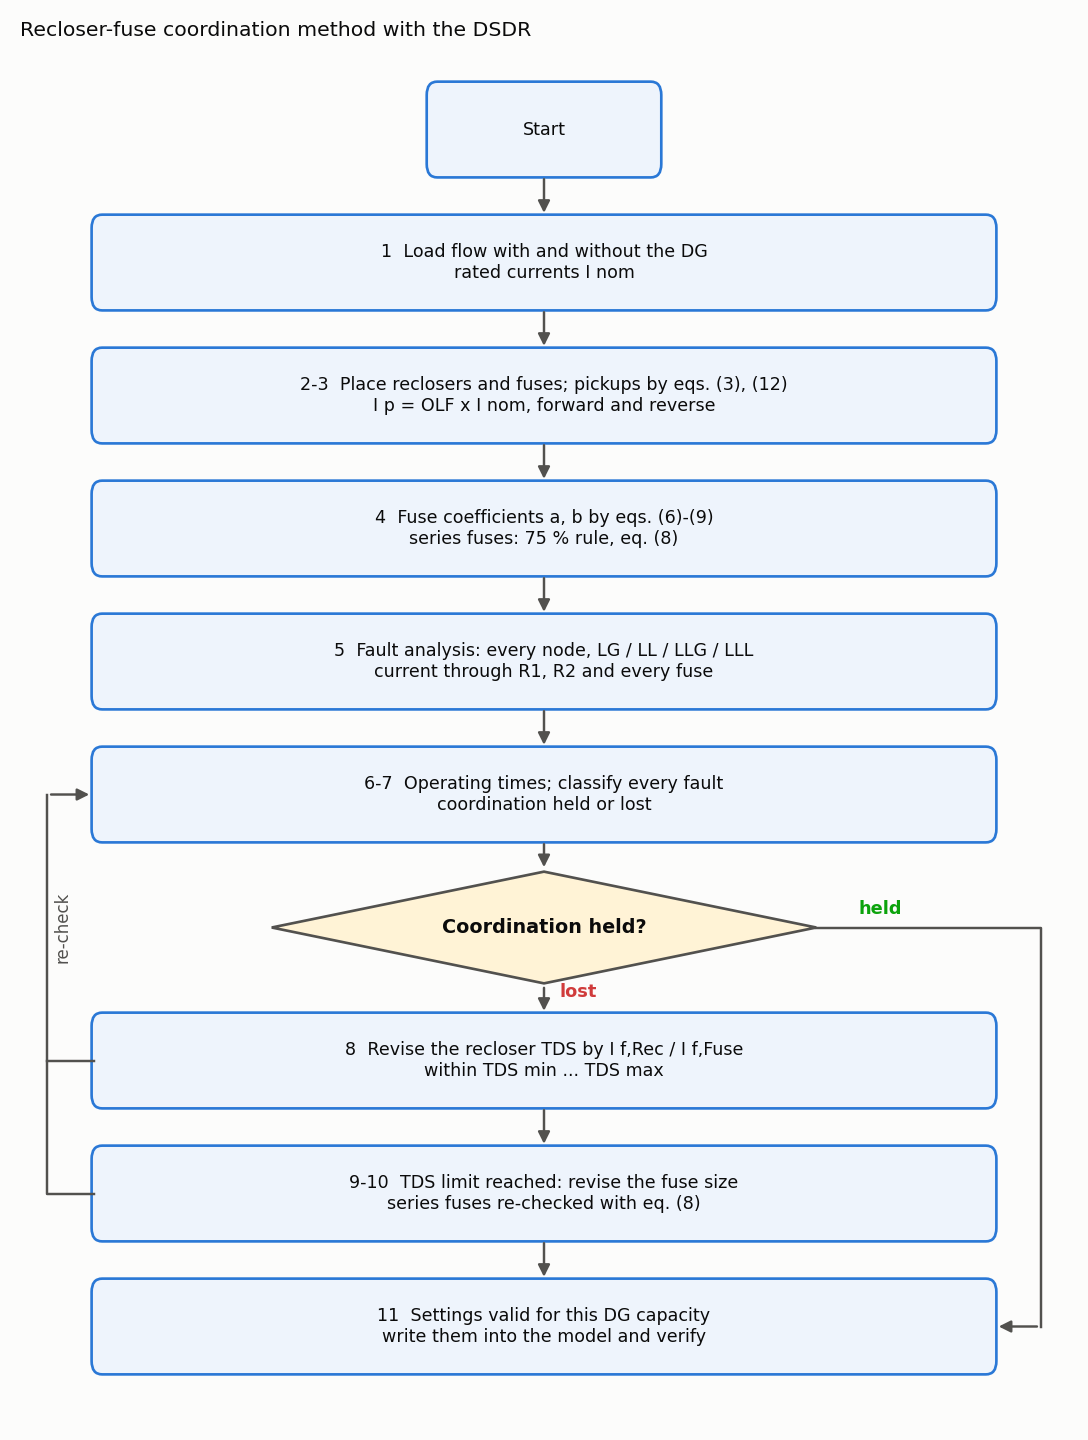
\includegraphics[height=0.64\textheight]{flowchart.png}
\caption{Flowchart of the recloser--fuse coordination method with the DSDR.}
\label{fig:flow}
\end{figure}

\subsection{Model Setup in DIgSILENT \PF}
The study is carried out in DIgSILENT \PF{} 2021~SP2~\cite{pf2021}. The feeder is the
IEEE 13-node model of the DIgSILENT example library; its lines, loads and regulator taps were checked against
the IEEE data. The study case that includes the 115/4.16\,kV, 5\,MVA substation transformer is used, because
it reproduces the IEEE short-circuit benchmark~\cite{kersting2012}.


\subsection{Load Flow Analysis}
The load flow is the unbalanced three-phase AC load flow of \PF. It gives the rated current of every
protected branch (largest phase), the bus voltages per phase, and the current and its direction at the two
reclosers with and without the DG.

\subsection{Recloser Pickup Current}
The method uses an overload factor of 1.25~\cite{yousaf2022}. The pickup is 1.25 times the rated current of the protected
branch, eq.~\eqref{eq:ipfw}, and is then set on the nearest available tap of the relay.

\subsection{Short-Circuit Analysis}
Short circuits are calculated with the \emph{complete method} of \PF, which starts from the pre-fault load
flow. LG, LL, LLG and LLL faults are applied at every node for every phase combination that exists there,
with the DG out and in. The maximum fault current of a branch is a bolted fault at its nearest node; the
minimum is an LG fault through 3\ohm{} at its farthest node~\cite{yousaf2022}. The current through R1, R2,
every fuse and every branch of Table~\ref{tab:t2} is stored for each fault.

\subsection{Mathematical Formulation of the DSDR}
\label{sec:dsdr}
The equations below are those of the reference method~\cite{yousaf2022}.

\subsubsection{Forward Fast and Delayed Operating Time}
\begin{equation}
t^{fw}_{k,l,F} = TDS^{fw}_{k,F}\left[\frac{A^{fw}_{k}}{\left(I_{f,l}/I^{fw}_{p,k}\right)^{n^{fw}_{k}}-1}+B^{fw}_{k}\right]
\label{eq:tf}
\end{equation}
\begin{equation}
t^{fw}_{k,l,D} = TDS^{fw}_{k,D}\left[\frac{A^{fw}_{k}}{\left(I_{f,l}/I^{fw}_{p,k}\right)^{n^{fw}_{k}}-1}+B^{fw}_{k}\right]
\label{eq:td}
\end{equation}
The fast and the delayed operation of recloser $k$ for a fault at location $l$ use the same curve with two
time dials. $I_{f,l}$ is the fault current through the recloser and $I_p$ its pickup.

\subsubsection{Forward Pickup Current and Constraints}
\begin{equation}
I^{fw}_{p,k} = OLF \times I^{fw}_{nom,k}
\label{eq:ipfw}
\end{equation}
\begin{equation}
TDS_{k,min} < TDS^{fw}_{k,F},\; TDS^{fw}_{k,D} < TDS_{k,max}
\label{eq:tdslim}
\end{equation}
\begin{equation}
I_{p,k,min} < I^{fw}_{p,k} < I_{p,k,max}
\label{eq:iplim}
\end{equation}
The pickup lies above the load current and below the minimum fault current of the zone; the dials must stay
inside the range of the device.

\subsubsection{Fuse Characteristic and Coefficient}
\begin{equation}
\log t_{fuse,i} = a_i \log I_{f,i} + b_i
\label{eq:fuse}
\end{equation}
\begin{equation}
b_i = \log\!\left[\frac{t^{fw}_{k,F}+t^{fw}_{k,D}}{2}\right] - a_i \log I_{f,i}
\label{eq:bi}
\end{equation}
with $a_i=-1.8$. Equation~\eqref{eq:bi} places a single fuse midway between the fast and the delayed time at
the calibration current.

\subsubsection{Series Fuses}
\begin{equation}
t_{TCT,\,i} \le 0.75\; t_{MMT,\,i+1}
\label{eq:75}
\end{equation}
\begin{equation}
b_i = \log\!\left[t^{fw}_{k,F}+\frac{i\left(t^{fw}_{k,D}-t^{fw}_{k,F}\right)}{z+1}\right] - a_i \log I_{f,i}
\label{eq:biseries}
\end{equation}
where $z$ is the number of series fuses in the fault path and $i=1$ is the fuse closest to the fault.
Equation~\eqref{eq:biseries} divides the window between the two recloser times among the series fuses.

\subsubsection{Reverse Operating Times, Pickup and Constraints}
\begin{equation}
t^{rv}_{k,m,F} = TDS^{rv}_{k,F}\left[\frac{A^{rv}_{k}}{\left(I_{f,m}/I^{rv}_{p,k}\right)^{n^{rv}_{k}}-1}+B^{rv}_{k}\right]
\label{eq:trf}
\end{equation}
\begin{equation}
t^{rv}_{k,m,D} = TDS^{rv}_{k,D}\left[\frac{A^{rv}_{k}}{\left(I_{f,m}/I^{rv}_{p,k}\right)^{n^{rv}_{k}}-1}+B^{rv}_{k}\right]
\label{eq:trd}
\end{equation}
\begin{equation}
I^{rv}_{p,k} = OLF \times I^{rv}_{nom,k}
\label{eq:iprv}
\end{equation}
\begin{equation}
TDS_{k,min} < TDS^{rv}_{k,F},\; TDS^{rv}_{k,D} < TDS_{k,max}
\end{equation}
\begin{equation}
I_{p,k,min} < I^{rv}_{p,k} < I_{p,k,max}
\end{equation}
Here $m$ is a fault location upstream of the recloser. The reverse current is the contribution of the DG, and
the reverse pickup is based on the reverse load current that flows when the DG exports towards the
substation.

\subsection{Device Characteristics Used in the Model}
\label{sec:curves}
The model uses the time--current curves of the \PF{} library types of the protection devices.

\subsubsection{R1: GE IAC77B801A}
The operating time of R1 follows the GE IAC extremely inverse characteristic. The manufacturer gives it as
$t = M_{TDS}\,[A + B/(M-C) + D/(M-C)^2 + E/(M-C)^3]$ with $A = 0.004$, $B = 0.638$, $C = 0.620$, $D = 1.787$
and $E = 0.246$~\cite{gemultilin}. With the constants of the \PF{} library type (the same values to four
digits) the curve is
\begin{equation}
t = TDS\left[0.004+\frac{0.6379}{M-0.62}+\frac{1.7872}{(M-0.62)^2}+\frac{0.2461}{(M-0.62)^3}\right],
\qquad M=\frac{I_f}{I_p},
\label{eq:iac}
\end{equation}
valid from $M=1.5$ to $M=40$. For 4219\,A, for example, it gives 0.096\,s (fast, TDS 0.5) and 1.926\,s
(delayed, TDS 10).

\subsubsection{R2: GE/Alstom CDG34}
The CDG extremely inverse characteristic is a manufacturer's table of time against $M=I_f/I_s$ for time
multipliers from 0.1 to 1.0. It starts at twice the plug setting and is interpolated on log-log axes:
\begin{equation}
t = t_1\left(\frac{t_2}{t_1}\right)^{f},\qquad f=\frac{\ln(M/M_1)}{\ln(M_2/M_1)} .
\label{eq:cdg}
\end{equation}
The table is not defined below a multiplier of 0.1, so 0.1 is the fastest setting of this relay.
The dial of R1 is called the time dial setting (TDS), as in the IAC77B801A documentation, whereas the CDG34
documentation calls the dial of R2 the time multiplier setting (TMS). Both scale the operating time of the
curve in the same way, and the general equations of Section~\ref{sec:dsdr} write TDS for either.

\subsubsection{Fuses}
The fuses are Gould-Shawmut A055C (5.5\,kV, E-rated) with their minimum-melting and total-clearing curves.
The fuse times are read from these curves at the current through the fuse with the same interpolation as
eq.~\eqref{eq:cdg}. The straight line of eq.~\eqref{eq:fuse} is used only to compute the coefficients of
Table~\ref{tab:t3}.

\subsection{Coordination Criteria}
A fault cell is classified as \emph{coordination exists} when all of the following hold:
\begin{equation}
t_{MMT}(I_{fuse}) > t_F \quad\text{for every recloser that feeds the fault through the fuse,}
\label{eq:crit1}
\end{equation}
\begin{equation}
t_{TCT}(I_{fuse}) < t_D \quad\text{for the same reclosers,}
\label{eq:crit2}
\end{equation}
together with the series-fuse condition of eq.~\eqref{eq:75} and a margin of at least 10~cycles
between the delayed curves of R2 and R1. The coordination time interval is $CTI = t_{MMT} - t_F$, the time by
which the fuse starts to melt after the latest fast trip; a cell is held when $CTI > 0$ (the zero-margin
criterion). A cell (node and fault type) is held only if every phase
combination of that fault type is held. The fuse and each recloser are evaluated at their own currents,
because with DG they differ.

\subsection{Design Procedure}
The flowchart of Figure~\ref{fig:flow} is applied in these steps.
\begin{enumerate}[itemsep=1pt]
\item Run the load flow without DG and set the recloser pickups from the rated currents.
\item Run the short-circuit study for the minimum and maximum fault currents of each section.
\item Set the dials: R1 at TDS 0.5 and 10; R2 fast at its lowest dial, delayed 10~cycles below R1.
\item Calculate the fuse coefficients and check the installed fuses, including the series fuses.
\item Classify the coordination without DG and revise the fuses until every case is held.
\item Connect the DG with the settings unchanged and classify again.
\item Set the reverse pickup and the reverse dials of R2 as a DSDR.
\item Revise the dials and, where a dial limit is reached, the fuse sizes until the cases are held.
\item Classify the coordination with the DSDR and determine the operating times.
\item Verify with \PF's own relay and fuse models and the EMT simulation.
\end{enumerate}

% =====================================================================================================
\chapterhead{FOUR}{SYSTEM MODELING AND SIMULATION SETUP}

\subsection{DIgSILENT \PF{} Environment}
The model is the project \emph{IEEE13 DSDR Fuse Coordination} in \PF{} 2021~SP2. Load flows use the
unbalanced AC method, short circuits the complete method, and the time-domain study the EMT simulation with a
step of 0.1\,ms. The relays and fuses are modelled with the \PF{} library types of the actual devices.

\subsection{IEEE 13-Node Feeder Model}
Figure~\ref{fig:sld} shows the feeder with its protection devices. The feeder has the
voltage regulator at the substation, overhead and cable sections, the 4.16/0.48\,kV transformer XFM-1, spot
and distributed loads, and two capacitors. The middle part of the distributed load on line 632--671 is placed
behind a short lateral (node DL) so that a fault there lies below its fuse.

\begin{figure}[H]
\centering
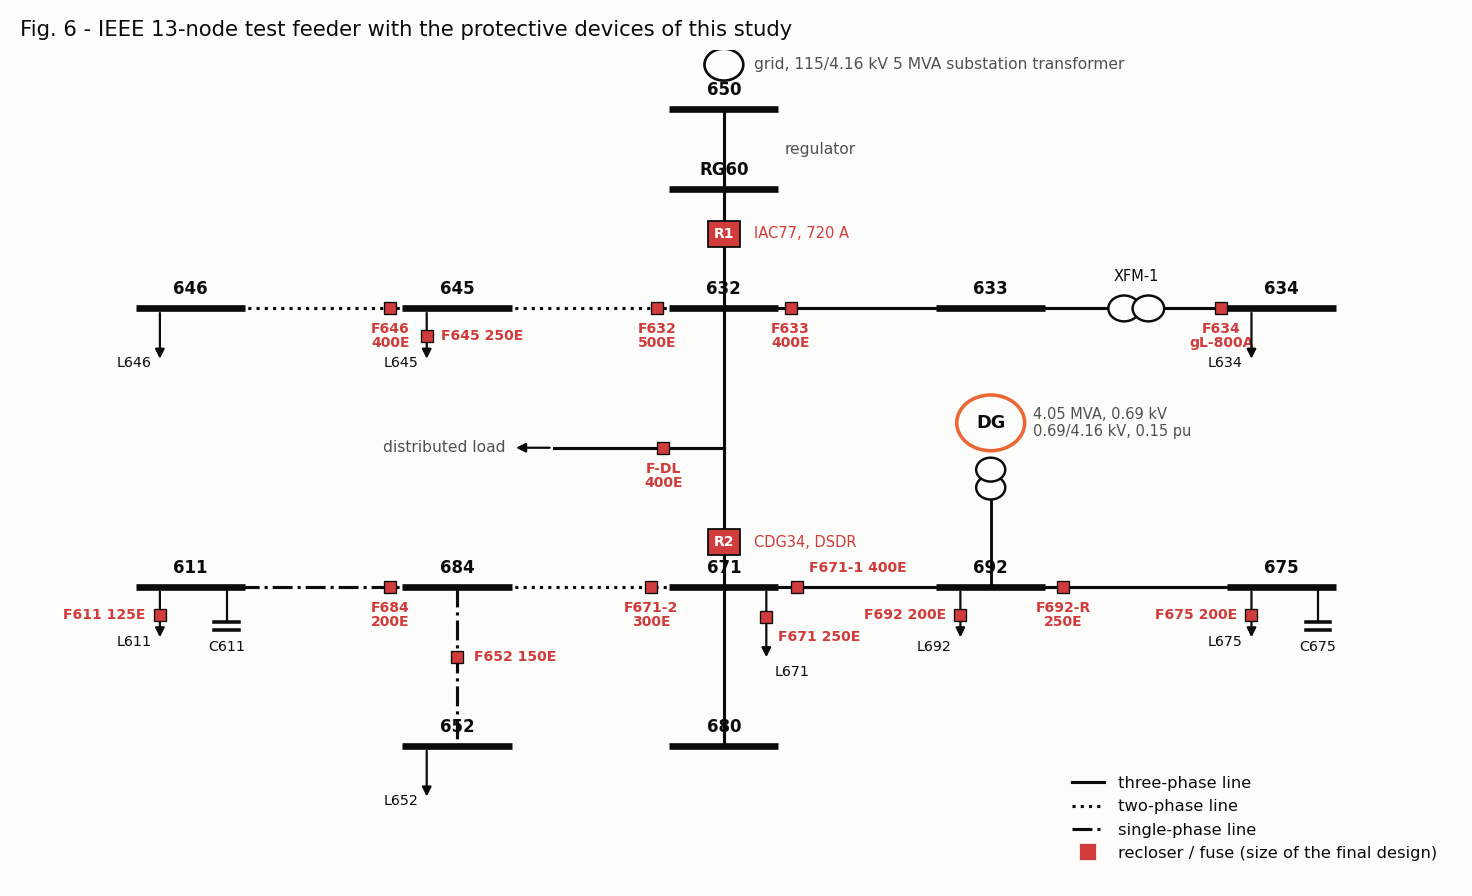
\includegraphics[width=\textwidth]{sld.png}
\caption{IEEE 13-node feeder with the reclosers R1 and R2, the fuses and the DG at node 692.}
\label{fig:sld}
\end{figure}

\subsection{Source and Feeder}
The source is an external grid at 115\,kV behind the 5\,MVA, 115/4.16\,kV substation transformer
($u_k = 8.06 per cent$). With this source the fault currents agree with the IEEE benchmark~\cite{kersting2012}
within about 2 per cent at every node. The alternative study case with a stiff 4.16\,kV source overstates the
fault levels by 20 to 65 per cent and is not used. The regulator taps are fixed at +10, +8 and +11.

\subsection{Distributed Generation Model}
The DG is a 4.05\,MVA, 0.69\,kV synchronous machine connected to node 692 through a 0.69/4.16\,kV
transformer with a leakage reactance of 0.15\,p.u. It is modelled with the standard synchronous-machine
model of \PF, round rotor, with the short-circuit data of Table~\ref{tab:dg} (values read back from the
model). In the load flow the machine delivers 3.24\,MW and controls its terminal voltage to 1.0\,p.u.

\begin{table}[H]
\centering\small
\begin{tabular}{|l|c|c|c|}
\hline
\textbf{Parameter} & \textbf{Symbol} & \textbf{Value} & \textbf{Unit} \\ \hline
Leakage reactance & $X_l$ & 0.05 & pu \\ \hline
Stator resistance & $R_a$ & 0.0014 & pu \\ \hline
d-axis synchronous reactance & $X_d$ & 1.4 & pu \\ \hline
d-axis transient reactance & $X'_d$ & 0.231 & pu \\ \hline
d-axis subtransient reactance & $X''_d$ & 0.118 & pu \\ \hline
d-axis transient open-circuit time constant & $T'_{d0}$ & 5.5 & s \\ \hline
d-axis subtransient open-circuit time constant & $T''_{d0}$ & 0.05 & s \\ \hline
q-axis synchronous reactance & $X_q$ & 1.372 & pu \\ \hline
q-axis transient reactance & $X'_q$ & 0.8 & pu \\ \hline
q-axis subtransient reactance & $X''_q$ & 0.118 & pu \\ \hline
q-axis transient open-circuit time constant & $T'_{q0}$ & 1.25 & s \\ \hline
q-axis subtransient open-circuit time constant & $T''_{q0}$ & 0.19 & s \\ \hline
Mechanical starting time & $M = 2H$ & 1.5 & s \\ \hline
DG rating & $S_n$ & 4.05 & MVA \\ \hline
DG voltage & $U_n$ & 0.69 & kV \\ \hline
Step-up transformer, HV side & $U_{HV}$ & 4.16 & kV \\ \hline
Step-up transformer leakage reactance & $x_T$ & 0.15 & pu \\ \hline
\end{tabular}
\caption{Parameters of the synchronous DG in the \PF{} model.}
\label{tab:dg}
\end{table}

\subsection{Recloser Model}
R1 is at the feeder head (RG60--632). R2 is on line 632--671 at the 671 end; it is the DSDR, because with the
DG at 692 it carries forward current for faults at 671 and beyond and reverse current for faults towards 632.
Table~\ref{tab:settings} gives the settings. The forward and the reverse group of R2 are four relay units of
the CDG34 library type on two current transformers.

\begin{table}[H]
\centering\small
\begin{tabularx}{\textwidth}{|l|L|l|l|l|}
\hline
\textbf{Recloser} & \textbf{Relay, CT} & \textbf{$1.25\,I_{nom}$} & \textbf{Setting} & \textbf{Dial fast / delayed} \\ \hline
R1 forward & GE IAC77B801A, 900/5 & 734.6\,A & tap 4\,A = 720\,A & TDS 0.5 / 10 \\ \hline
R2 forward & CDG34, 1000/5 & 587.5\,A & plug 300\,A / 600\,A & TMS 0.1 / 1.0 \\ \hline
R2 reverse & CDG34, 500/5 & 315.3\,A & plug 150\,A / 300\,A & TMS 0.1 / 1.0 \\ \hline
\end{tabularx}
\caption{Recloser settings. For R2 the fast plug is half and the delayed plug equal to $1.25\,I_{nom}$, because
the CDG curve starts at twice the plug setting.}
\label{tab:settings}
\end{table}

\subsection{Fuse Model}
Table~\ref{tab:fuses} lists the fifteen fuses. The starting size is the size drawn in the figures of the
reference paper where a figure shows the fuse (the fuse bands were digitised and matched to the A055C
library curves within 2 per cent), otherwise the size of the benchmark scheme~\cite{yousaf2020}. The last two
columns are the sizes after the fuse revision of the method without DG and with the DSDR.

\begin{table}[H]
\centering\footnotesize
\begin{tabularx}{\textwidth}{|l|l|c|c|c|L|}
\hline
\textbf{Fuse} & \textbf{Location} & \textbf{Start} & \textbf{No DG} & \textbf{DSDR} & \textbf{Source of the starting size} \\ \hline
F632 & lateral 632--645, at 632 & 400E & 400E & \textbf{500E} & Ref.~\cite{yousaf2022}, Figs. 12, 15, 16 \\ \hline
F633 & lateral 632--633, at 632 & 250E & 250E & \textbf{400E} & Benchmark scheme~\cite{yousaf2020}, Table V \\ \hline
F634 & XFM-1, 0.48 kV side & gL-800A & gL-800A & gL-800A & Benchmark scheme~\cite{yousaf2020}, Table V \\ \hline
F645 & load at 645 & 250E & 250E & 250E & Benchmark scheme~\cite{yousaf2020}, Table V \\ \hline
F646 & line 645--646, at 645 & 300E & 300E & \textbf{400E} & Ref.~\cite{yousaf2022}, Figs. 11, 15, 16 \\ \hline
F-DL & distributed-load lateral on 632--671 & 250E & 250E & \textbf{400E} & Benchmark scheme~\cite{yousaf2020}, Table V \\ \hline
F671 & load at 671 & 250E & 250E & 250E & Benchmark scheme~\cite{yousaf2020}, Table V \\ \hline
F671-1 & 671--692 (switch), at 671 & 300E & 300E & \textbf{400E} & Ref.~\cite{yousaf2022}, Fig. 9 \\ \hline
F692 & load at 692 & 200E & 200E & 200E & Benchmark scheme~\cite{yousaf2020}, Table V \\ \hline
F692-R & cable 692--675, at 692 & 250E & 200E & \textbf{250E} & Ref.~\cite{yousaf2022}, Fig. 9 \\ \hline
F675 & load at 675 & 200E & 200E & 200E & Benchmark scheme~\cite{yousaf2020}, Table V \\ \hline
F671-2 & lateral 671--684, at 671 & 300E & 300E & 300E & Ref.~\cite{yousaf2022}, Fig. 8 \\ \hline
F684 & line 684--611, at 684 & 200E & 200E & 200E & Ref.~\cite{yousaf2022}, Fig. 8 \\ \hline
F611 & load at 611 & 125E & 125E & 125E & Benchmark scheme~\cite{yousaf2020}, Table V \\ \hline
F652 & cable 684--652, at 684 & 150E & 150E & 150E & Benchmark scheme~\cite{yousaf2020}, Table V \\ \hline
\end{tabularx}
\caption{Fuses and their sizes (A055C, E-rated). Bold: changed by the fuse revision with the DG.}
\label{tab:fuses}
\end{table}

\subsection{Fault Model}
Faults are applied at the nodes 632, 633, 634, 645, 646, DL, 671, 692, 675, 680, 684, 611 and 652. Only the
fault types that the phases of a node allow are applied, for example LL and LLG on phases b--c at 645 and
646, and LG only at 611 and 652. This gives 39 node/fault-type cells. Selected faults
through a fault impedance are added for the time--current figures.

\subsection{Measurement and Data Acquisition}
\label{sec:assumptions}
For every fault the phase currents through R1, R2 and each fuse are read from the short-circuit result. The
operating current of a device is its largest phase current. The forward direction is away from the grid; R2
sits at the 671 end of its line, where \PF{} counts the current positive into the line, so its values are
multiplied by $-1$. The following modelling choices were made:
\begin{itemize}
\item the source: the IEEE benchmark substation transformer, with the complete short-circuit method;
\item R1: tap 4\,A on a 900/5 current transformer, i.e.\ a pickup of 720\,A;
\item R2: all settings of Table~\ref{tab:settings}, derived from eqs.~\eqref{eq:ipfw} and \eqref{eq:iprv};
\item the operating-time cases of Table~\ref{tab:t4a}: bolted LLL faults, LL at two-phase nodes, LG at single-phase nodes;
\item the EMT study: a reclosing dead time of 0.2\,s and a breaker time of three cycles.
\end{itemize}

\subsection{Simulation Cases}
\begin{table}[H]
\centering\small
\begin{tabularx}{\textwidth}{|l|l|L|L|}
\hline
\textbf{Case} & \textbf{DG} & \textbf{Faults} & \textbf{Purpose} \\ \hline
Load flow & out / in & -- & Rated currents, voltages, direction at R1 and R2 \\ \hline
Maximum faults & out / in & All nodes, LG/LL/LLG/LLL, all phase combinations, bolted & Classification, Tables II--IV \\ \hline
Minimum faults & out / in & LG through 3\ohm{} at all nodes & $I_{f,min}$, pickup check \\ \hline
Figure faults & in & Selected faults, bolted and through a fault impedance & Time--current figures \\ \hline
EMT & out / in & LL a--c at 684 through 0.2\ohm & Reclosing sequence \\ \hline
Penetration & 0--100\,\% & LLL at 633, LL at 684, all nodes & CTI, fault levels and pickups against DG size \\ \hline
\end{tabularx}
\caption{Simulation cases.}
\label{tab:cases}
\end{table}

% =====================================================================================================
\chapterhead{FIVE}{RESULTS OBTAINED}

\subsection{Load-Flow Results}
Table~\ref{tab:volt} gives the bus voltages with and without the DG. Without DG the lowest voltage is
0.971\,p.u. (phase c at 611). The DG raises the voltages of the loaded phases a and c at node 671 and beyond
by about 0.03 to 0.05\,p.u.

\begin{table}[H]
\centering\small
\begin{tabular}{|l|c|c|c|c|c|c|}
\hline
 & \multicolumn{3}{c|}{\textbf{Without DG (p.u.)}} & \multicolumn{3}{c|}{\textbf{With DG (p.u.)}} \\
\textbf{Bus} & \textbf{A} & \textbf{B} & \textbf{C} & \textbf{A} & \textbf{B} & \textbf{C} \\ \hline
650 & 0.9981 & 1.0170 & 0.9979 & 1.0084 & 1.0200 & 1.0057 \\ \hline
RG60 & 1.0605 & 1.0679 & 1.0665 & 1.0715 & 1.0710 & 1.0748 \\ \hline
632 & 1.0187 & 1.0616 & 1.0142 & 1.0482 & 1.0640 & 1.0361 \\ \hline
633 & 1.0158 & 1.0588 & 1.0124 & 1.0454 & 1.0611 & 1.0344 \\ \hline
634 & 0.9918 & 1.0406 & 0.9936 & 1.0221 & 1.0430 & 1.0161 \\ \hline
645 & -- & 1.0540 & 1.0106 & -- & 1.0563 & 1.0325 \\ \hline
646 & -- & 1.0522 & 1.0085 & -- & 1.0546 & 1.0304 \\ \hline
DL & 1.0028 & 1.0666 & 0.9939 & 1.0407 & 1.0685 & 1.0221 \\ \hline
671 & 0.9877 & 1.0722 & 0.9753 & 1.0334 & 1.0738 & 1.0094 \\ \hline
692 & 0.9877 & 1.0722 & 0.9753 & 1.0334 & 1.0738 & 1.0094 \\ \hline
675 & 0.9809 & 1.0767 & 0.9729 & 1.0271 & 1.0781 & 1.0072 \\ \hline
680 & 0.9877 & 1.0722 & 0.9753 & 1.0334 & 1.0738 & 1.0094 \\ \hline
684 & 0.9859 & -- & 0.9732 & 1.0315 & -- & 1.0074 \\ \hline
652 & 0.9811 & -- & -- & 1.0265 & -- & -- \\ \hline
611 & -- & -- & 0.9712 & -- & -- & 1.0055 \\ \hline
\end{tabular}
\caption{Bus voltages from the unbalanced load flow, without and with the DG.}
\label{tab:volt}
\end{table}

Table~\ref{tab:lf} shows the load current at the two reclosers. With the DG the current through R2 reverses:
252.2\,A flows from 671 towards 632. This reverse load current is the basis of the reverse pickup,
eq.~\eqref{eq:iprv}.

\begin{table}[H]
\centering\small
\begin{tabular}{|l|c|c|c|c|}
\hline
\textbf{Device} & \textbf{Without DG (A)} & \textbf{Direction} & \textbf{With DG (A)} & \textbf{Direction} \\ \hline
R1 & $+587.7$ & forward & $+284.9$ & forward \\ \hline
R2 & $+470.0$ & forward & $-252.2$ & reverse \\ \hline
\end{tabular}
\caption{Load current at the reclosers (largest phase; + is forward, away from the grid).}
\label{tab:lf}
\end{table}

\subsection{Branch Currents and Fault Levels}
Table~\ref{tab:t2} gives the rated current of every protected branch from the unbalanced load flow, the
minimum fault current (LG through 3\ohm{} at the farthest node of the branch's section) and the maximum
fault current (bolted, nearest node). The largest fault current at the feeder head is 4.73\,kA; the fault
levels agree with the IEEE 13-node short-circuit benchmark within about 2 per cent.

\begin{table}[H]
\centering\footnotesize
\begin{tabular}{|l|c|c|c|}
\hline
\textbf{Branch} & \textbf{$I_{nom}$ (A)} & \textbf{$I_{f,min}$ (kA)} & \textbf{$I_{f,max}$ (kA)} \\ \hline
RG60--632 & 587.7 & 1.07 & 4.73 \\ \hline
632--633 & 81.0 & 0.76 & 4.1 \\ \hline
632--645 & 143.1 & 0.73 & 3.42 \\ \hline
632--671 & 470.0 & 0.88 & 3.39 \\ \hline
XFM1-HV side & 81.0 & 0.08 & 1.81 \\ \hline
XFM1-LV side & 706.4 & 0.71 & 15.67 \\ \hline
645--646 & 66.1 & 0.73 & 3.11 \\ \hline
671--692 & 229.7 & 0.74 & 3.39 \\ \hline
671--684 & 71.1 & 0.66 & 2.66 \\ \hline
671--680 & 0.0 & 0.64 & 2.93 \\ \hline
692--675 & 205.9 & 0.74 & 3.15 \\ \hline
684--611 & 71.1 & 0.68 & 1.86 \\ \hline
684--652 & 63.0 & 0.66 & 1.87 \\ \hline
\end{tabular}
\caption{Rated, minimum and maximum fault current of the protected branches without DG. XFM1 HV side: 4.16\,kV
currents for a fault on the 0.48\,kV side.}
\label{tab:t2}
\end{table}

\subsection{Recloser Pickup Currents and Settings}
With the rated currents of Table~\ref{tab:t2}, eq.~\eqref{eq:ipfw} gives 734.6\,A for R1 and 587.5\,A for R2
forward. The settings actually applied are those of Table~\ref{tab:settings}. Without DG both pickups are
below the lowest minimum fault current of their zones (1074\,A and 879\,A).

\subsection{Short-Circuit Results With and Without DG}
Table~\ref{tab:fault} gives the largest fault current at each node and the current through the two reclosers.
The DG raises the fault current at every node, by 38 per cent at 632 and by 64 per cent at 671. For faults at 632,
633, 645, 646 and DL the current through R2 becomes negative: R2 then carries only the DG contribution, 1.1
to 2.0\,kA, in the reverse direction, while R1 still carries the grid contribution.

\begin{table}[H]
\centering\footnotesize
\begin{tabular}{|l|l|c|c|c|c|c|c|}
\hline
 & & \multicolumn{2}{c|}{\textbf{$I_{f,max}$ at the fault (A)}} & \multicolumn{2}{c|}{\textbf{Through R1 (A)}} & \multicolumn{2}{c|}{\textbf{Through R2 (A)}} \\
\textbf{Bus} & \textbf{Fault} & \textbf{no DG} & \textbf{DG} & \textbf{no DG} & \textbf{DG} & \textbf{no DG} & \textbf{DG} \\ \hline
632 & LLL ABC & 4735 & 6526 & $+4735$ & $+4734$ & $+0$ & $-1813$ \\ \hline
633 & LLL ABC & 4102 & 5426 & $+4162$ & $+3970$ & $+66$ & $-1500$ \\ \hline
634 & LLL ABC & 15671 & 17608 & $+2034$ & $+1611$ & $+298$ & $-618$ \\ \hline
645 & LLG BC & 3418 & 4341 & $+3528$ & $+3330$ & $+478$ & $-1262$ \\ \hline
646 & LLG BC & 3112 & 3854 & $+3192$ & $+3000$ & $+475$ & $-1135$ \\ \hline
671 & LLL ABC & 3390 & 5564 & $+3413$ & $+3412$ & $+3390$ & $+3391$ \\ \hline
692 & LLL ABC & 3390 & 5564 & $+3413$ & $+3412$ & $+3390$ & $+3391$ \\ \hline
675 & LLL ABC & 3151 & 5022 & $+3202$ & $+3090$ & $+3174$ & $+3050$ \\ \hline
680 & LLL ABC & 2930 & 4460 & $+3006$ & $+2789$ & $+2976$ & $+2757$ \\ \hline
684 & LLG AC & 2655 & 4107 & $+2836$ & $+2669$ & $+2744$ & $+2651$ \\ \hline
652 & LG A & 1874 & 2239 & $+2094$ & $+1795$ & $+2059$ & $+1761$ \\ \hline
611 & LG C & 1857 & 2236 & $+2084$ & $+1814$ & $+1991$ & $+1718$ \\ \hline
DL & LLL ABC & 3946 & 5902 & $+3959$ & $+3954$ & $+1$ & $-1972$ \\ \hline
\end{tabular}
\caption{Maximum fault current and recloser currents without and with the DG (+ forward, $-$ reverse).}
\label{tab:fault}
\end{table}

\subsection{Fuse Coefficients}
Table~\ref{tab:t3} gives the fuse coefficients of eq.~\eqref{eq:biseries}, with $i = 1$ for the fuse closest
to the fault. The last columns give the installed fuse and its melting time at the same current; it is much
shorter than the time the equation asks for, because real fuse curves are steeper than the slope $-1.8$.

\begin{table}[H]
\centering\footnotesize
\begin{tabular}{|l|c|c|c|c|c|c|c|c|}
\hline
\textbf{Fuse} & \textbf{$I_f$ (A)} & \textbf{$i/z$} & \textbf{$t_F$ (s)} & \textbf{$t_D$ (s)} & \textbf{$t_{fuse}$ (s)} &
\textbf{$b_i$} & \textbf{Size} & \textbf{$t_{MMT}$ (s)} \\ \hline
F632 & 3418 & 2/2 & 0.133 & 2.670 & 1.824 & 6.62 & 400E & 0.512 \\ \hline
F633 & 4102 & 1/1 & 0.100 & 2.008 & 1.054 & 6.53 & 250E & 0.102 \\ \hline
F634 & 15671 & 1/2 & 0.439 & 8.772 & 3.217 & 8.06 & gL-800A & 0.021 \\ \hline
F645 & 3418 & 1/2 & 0.133 & 2.670 & 0.979 & 6.35 & 250E & 0.158 \\ \hline
F646 & 3112 & 1/2 & 0.156 & 3.115 & 1.142 & 6.35 & 300E & 0.273 \\ \hline
F-DL & 3946 & 1/1 & 0.106 & 2.130 & 1.118 & 6.52 & 250E & 0.112 \\ \hline
F671 & 3390 & 1/1 & 0.054 & 1.601 & 0.827 & 6.27 & 250E & 0.161 \\ \hline
F671-1 & 3390 & 3/3 & 0.054 & 1.601 & 1.214 & 6.44 & 300E & 0.218 \\ \hline
F692 & 3390 & 1/2 & 0.054 & 1.601 & 0.569 & 6.11 & 200E & 0.094 \\ \hline
F692-R & 3151 & 2/3 & 0.057 & 1.829 & 0.943 & 6.27 & 200E & 0.112 \\ \hline
F675 & 3151 & 1/3 & 0.057 & 1.829 & 0.500 & 6.00 & 200E & 0.112 \\ \hline
F671-2 & 2655 & 3/3 & 0.069 & 2.572 & 1.946 & 6.45 & 300E & 0.428 \\ \hline
F684 & 1857 & 2/3 & 0.113 & 5.778 & 2.946 & 6.35 & 200E & 0.465 \\ \hline
F611 & 1857 & 1/3 & 0.113 & 5.778 & 1.530 & 6.07 & 125E & 0.120 \\ \hline
F652 & 1874 & 1/2 & 0.112 & 5.660 & 1.961 & 6.18 & 150E & 0.207 \\ \hline
\end{tabular}
\caption{Fuse coefficients, eq.~\eqref{eq:bi}, $a_i=-1.8$. Size and $t_{MMT}$: fuse of the design without DG at the same
current.}
\label{tab:t3}
\end{table}

\subsection{Conventional Coordination Without DG}
With the starting fuse sizes 35 of the 39 cells are coordinated. The four lost cells are the faults
at 675, where the series fuses F692-R (250E) and F671-1 (300E) are not selective: F692-R does not
clear the fault early enough before F671-1 starts to melt. The fuse revision of
the method changes F692-R to 200E, after which all 39 cells are coordinated. Figures~\ref{fig:f8}
and \ref{fig:f9} show two cases: R2's fast curve lies below the fuses and its delayed curve
above them. In every time--current plot of this chapter the dotted lines carry each operating point to the time axis
with its operating time. The arrow at the fuse current gives the coordination time interval
$\mathrm{CTI} = t_{MMT} - t_F$ (green when positive, red when the fuse melts first) and the margin
$t_D - t_{TCT}$ by which the fuse clears before the delayed trip.

\begin{figure}[H]
\centering
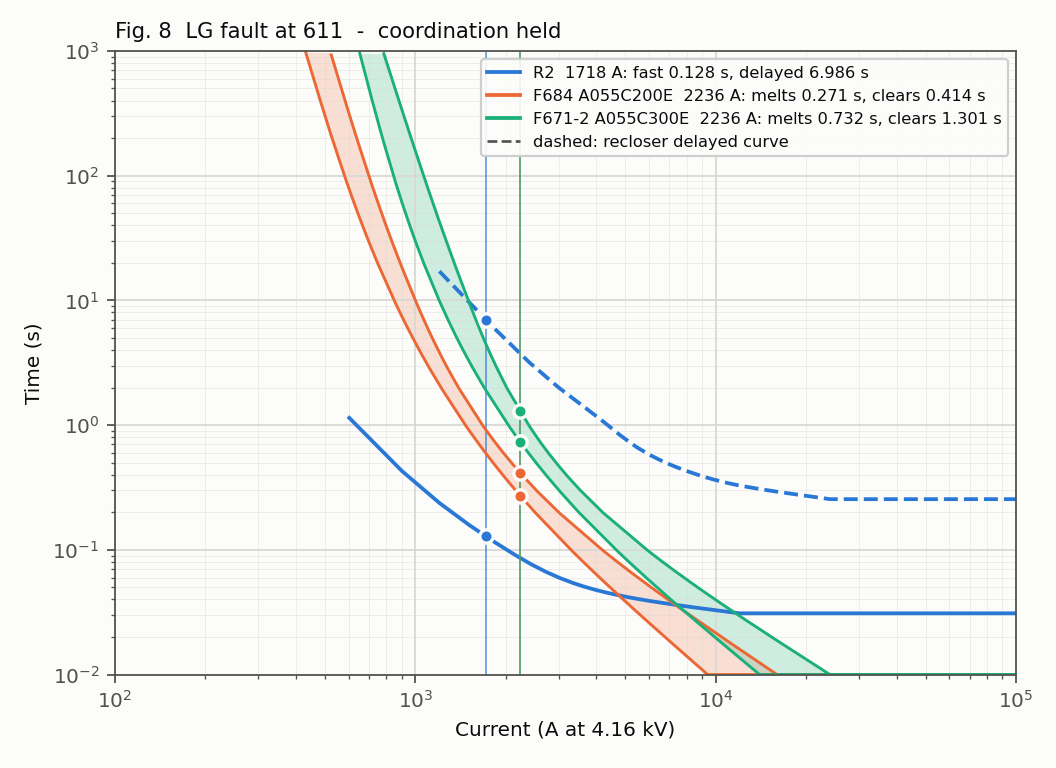
\includegraphics[width=0.68\textwidth]{fig08.png}
\caption{LG fault at 611: R2 forward, fuses F684 and F671-2; CTI = +143\,ms.}
\label{fig:f8}
\end{figure}

\begin{figure}[H]
\centering
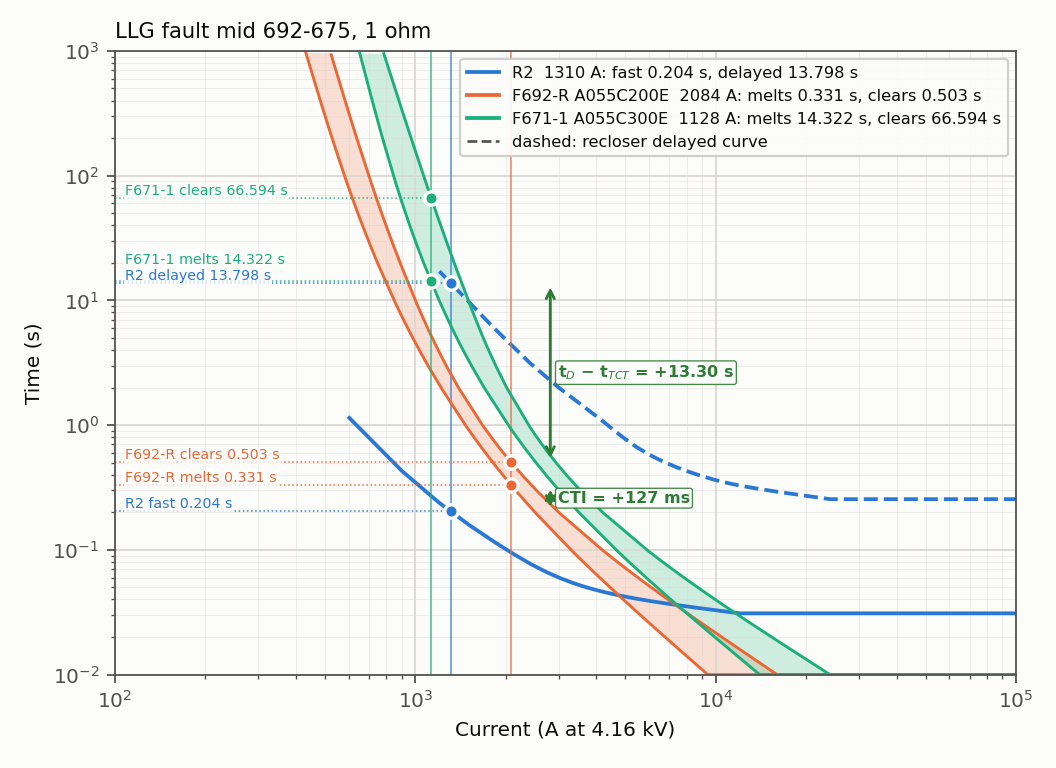
\includegraphics[width=0.68\textwidth]{fig09.png}
\caption{LLG fault at the middle of 692--675 through 1\ohm{}; CTI = +127\,ms.}
\label{fig:f9}
\end{figure}

\subsection{Coordination With DG and a Conventional R2}
With the DG connected and the settings unchanged, coordination is held in 24 of 39 cells
(Table~\ref{tab:g14}, Figure~\ref{fig:f14}). The lost cells are at 633, 645, 646, DL and 675: the fuse now
carries the grid and the DG current and melts before the fast trip, and for some LG faults the single-setting
R2 does not pick up the reverse DG current at all. At 633 and DL the fuses have almost no margin even
without DG, so every fault type is lost there.

\begin{table}[H]
\centering\footnotesize
\setlength{\tabcolsep}{4.5pt}
\begin{tabular}{|l|c|c|c|c|c|c|c|c|c|c|c|c|}
\hline
\textbf{Fault} & 632 & 633 & 645 & 646 & DL & 671 & 692 & 675 & 680 & 684 & 611 & 652 \\ \hline
LG & \ok & \no & \no & \no & \no & \ok & \ok & \ok & \ok & \ok & \ok & \ok \\ \hline
LL & \ok & \no & \ok & \no & \no & \ok & \ok & \no & \ok & \ok & -- & -- \\ \hline
LLG & \ok & \no & \ok & \no & \no & \ok & \ok & \no & \ok & \ok & -- & -- \\ \hline
LLL & \ok & \no & -- & -- & \no & \ok & \ok & \no & \ok & -- & -- & -- \\ \hline
\end{tabular}
\caption{Coordination status with DG and a conventional R2. $\checkmark$ exists, $\times$ does not exist,
-- not applicable.}
\label{tab:g14}
\end{table}

\begin{figure}[H]
\centering
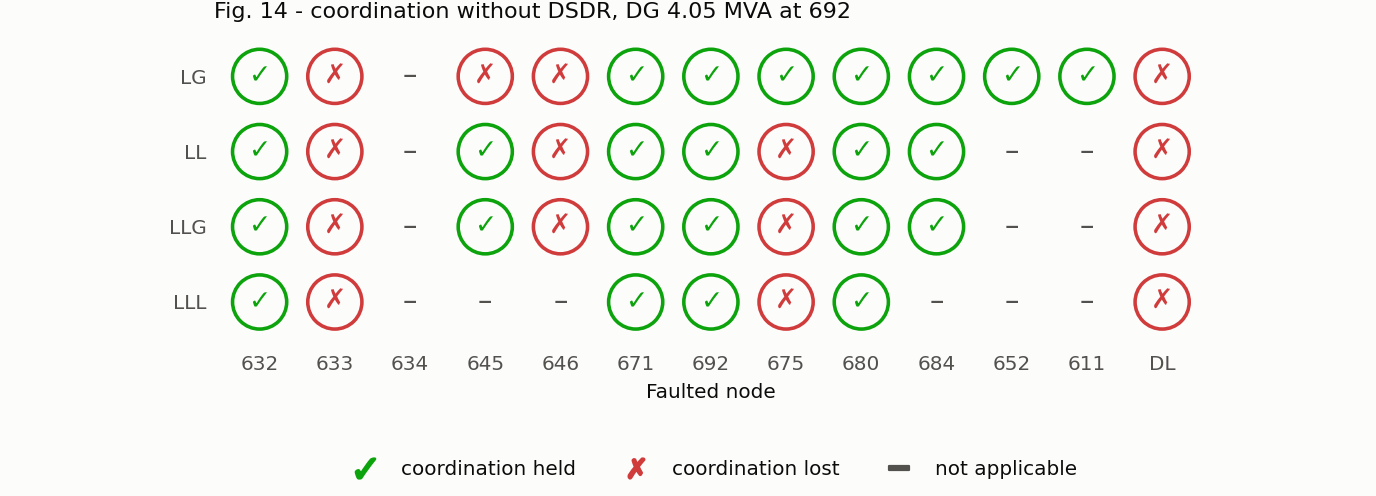
\includegraphics[width=0.9\textwidth]{fig14.png}
\caption{Coordination status with DG, without the DSDR.}
\label{fig:f14}
\end{figure}

Figures~\ref{fig:f11} to \ref{fig:f13} show three cases with the conventional R2.

\begin{figure}[H]
\centering
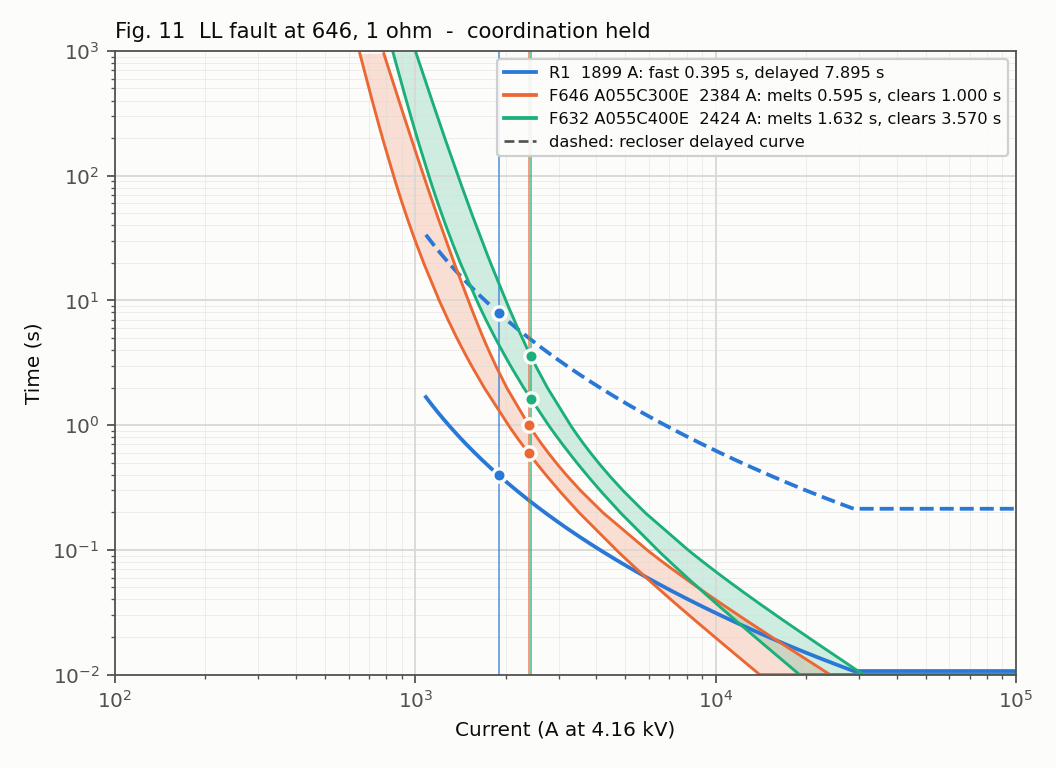
\includegraphics[width=0.68\textwidth]{fig11.png}
\caption{LL fault at 646 through 1\ohm: R1 with F646 and F632; CTI = +200\,ms.}
\label{fig:f11}
\end{figure}

\begin{figure}[H]
\centering
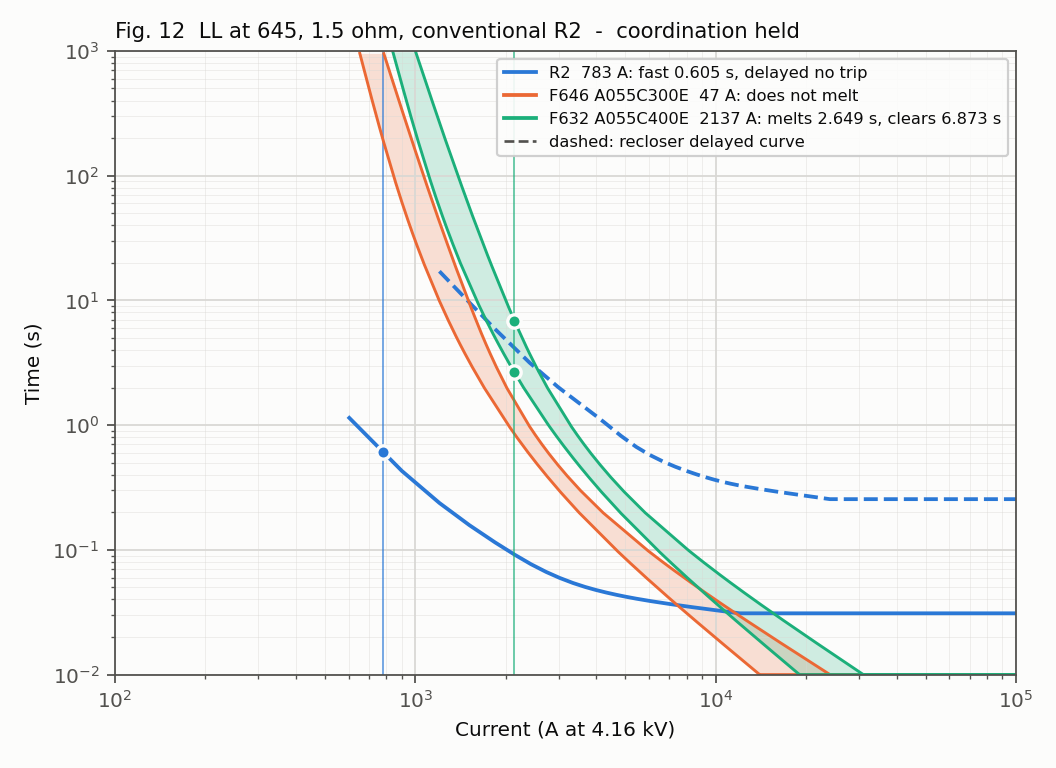
\includegraphics[width=0.68\textwidth]{fig12.png}
\caption{LL fault at 645 through 1.5\ohm, conventional R2.}
\label{fig:f12}
\end{figure}

\begin{figure}[H]
\centering
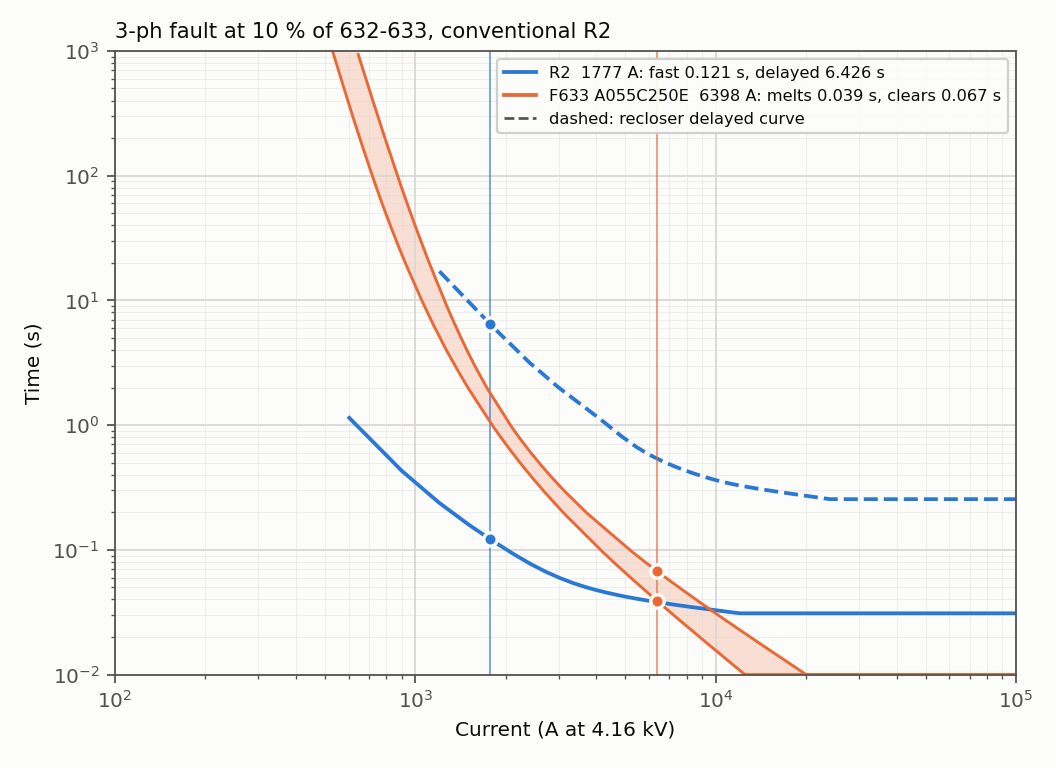
\includegraphics[width=0.68\textwidth]{fig13.png}
\caption{Three-phase fault at 10 per cent of line 632--633, conventional R2; CTI = $-83$\,ms, the fuse melts first.}
\label{fig:f13}
\end{figure}

\subsection{DSDR Settings and Fuse Revision}
The reverse load current of R2 is 252.2\,A, so eq.~\eqref{eq:iprv} gives a reverse pickup of 315.3\,A. The
reverse group is set on a 500/5 current transformer with plugs of 150\,A (fast) and 300\,A (delayed) and the
same time multipliers 0.1 and 1.0 (Figure~\ref{fig:f3}). Step~8 of the method (revising the dials) could not
improve any lost case, because R1 is already at both ends of the IAC dial range (0.5 and 10) and R2 at both
ends of the CDG table (0.1 and 1.0). Step~9 (revising the fuses) was therefore needed: F632 to 500E; F633,
F646, F-DL and F671-1 to 400E; F692-R to 250E (Table~\ref{tab:fuses}).

\begin{figure}[H]
\centering
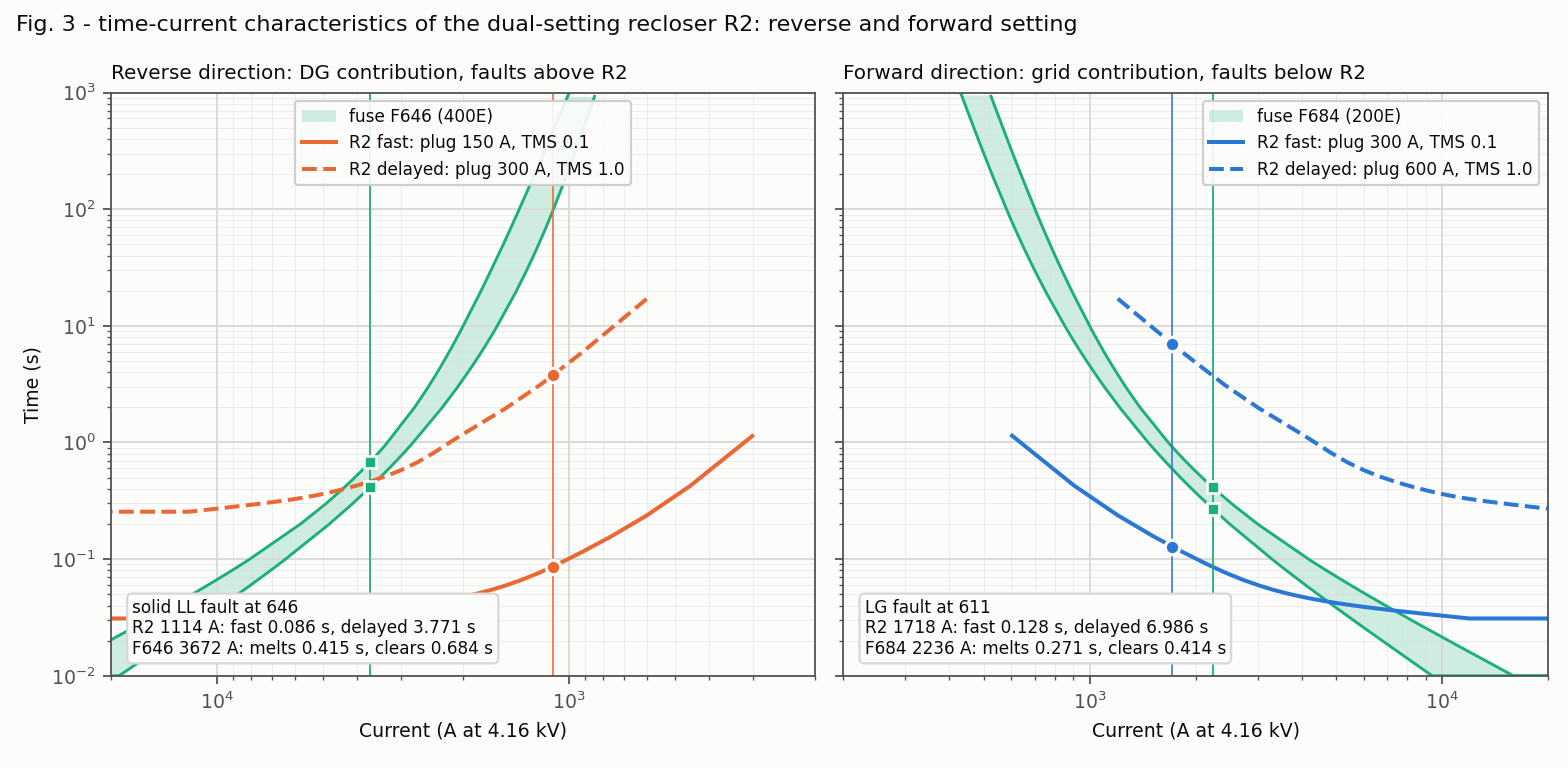
\includegraphics[width=\textwidth]{fig03.png}
\caption{The two setting groups of R2: reverse (DG contribution, faults towards 632) and forward (grid
contribution, faults beyond 671), each with one fault of the model.}
\label{fig:f3}
\end{figure}

\subsection{Coordination With the DSDR}
With R2 as a DSDR and the revised fuses, coordination is held in 38 of 39 cells
(Table~\ref{tab:g17}, Figure~\ref{fig:f17}). With the same revised fuses but a single-setting R2 only
31 cells are held. The dual setting itself therefore restores seven cells: all four fault types at
633, and the LG faults at 645, 646 and DL.

The cell that remains lost is the LG fault at 692. F671-1 must be 400E to stay selective with F692-R, but it
then clears after R2's delayed trip (7.6\,s against 4.0\,s), and R2's delayed dial is already at its maximum.

\begin{table}[H]
\centering\footnotesize
\setlength{\tabcolsep}{4.5pt}
\begin{tabular}{|l|c|c|c|c|c|c|c|c|c|c|c|c|}
\hline
\textbf{Fault, R2} & 632 & 633 & 645 & 646 & DL & 671 & 692 & 675 & 680 & 684 & 611 & 652 \\ \hline
LG, single setting & \ok & \no & \no & \no & \no & \ok & \no & \ok & \ok & \ok & \ok & \ok \\ \hline
LG, dual setting & \ok & \ok & \ok & \ok & \ok & \ok & \no & \ok & \ok & \ok & \ok & \ok \\ \hline
LL, single setting & \ok & \no & \ok & \ok & \ok & \ok & \ok & \ok & \ok & \ok & -- & -- \\ \hline
LL, dual setting & \ok & \ok & \ok & \ok & \ok & \ok & \ok & \ok & \ok & \ok & -- & -- \\ \hline
LLG, single setting & \ok & \no & \ok & \ok & \ok & \ok & \ok & \ok & \ok & \ok & -- & -- \\ \hline
LLG, dual setting & \ok & \ok & \ok & \ok & \ok & \ok & \ok & \ok & \ok & \ok & -- & -- \\ \hline
LLL, single setting & \ok & \no & -- & -- & \ok & \ok & \ok & \ok & \ok & -- & -- & -- \\ \hline
LLL, dual setting & \ok & \ok & -- & -- & \ok & \ok & \ok & \ok & \ok & -- & -- & -- \\ \hline
\end{tabular}
\caption{Coordination status with DG and the revised fuses: single-setting R2 against dual-setting R2.}
\label{tab:g17}
\end{table}

\begin{figure}[H]
\centering
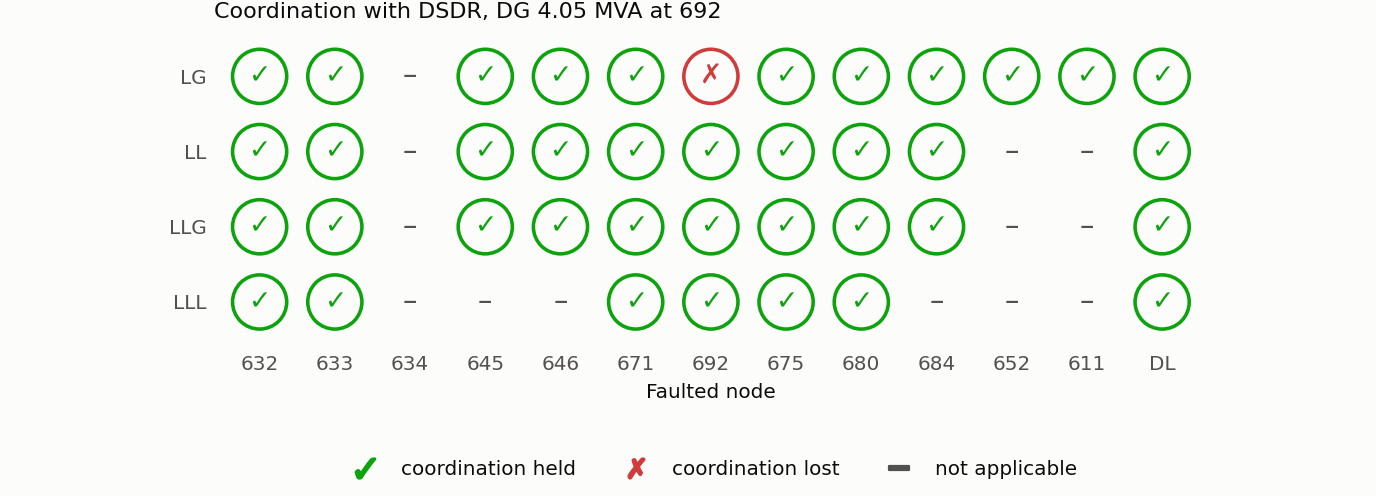
\includegraphics[width=0.9\textwidth]{fig17.png}
\caption{Coordination status with DG and the DSDR.}
\label{fig:f17}
\end{figure}

Figures~\ref{fig:f15} and \ref{fig:f16} show a bolted LL fault at 646. The fuses carry 3.67\,kA. R2 carries
1.11\,kA in reverse and trips on its reverse fast curve in 0.086\,s, before F646 melts (0.415\,s).

\begin{figure}[H]
\centering
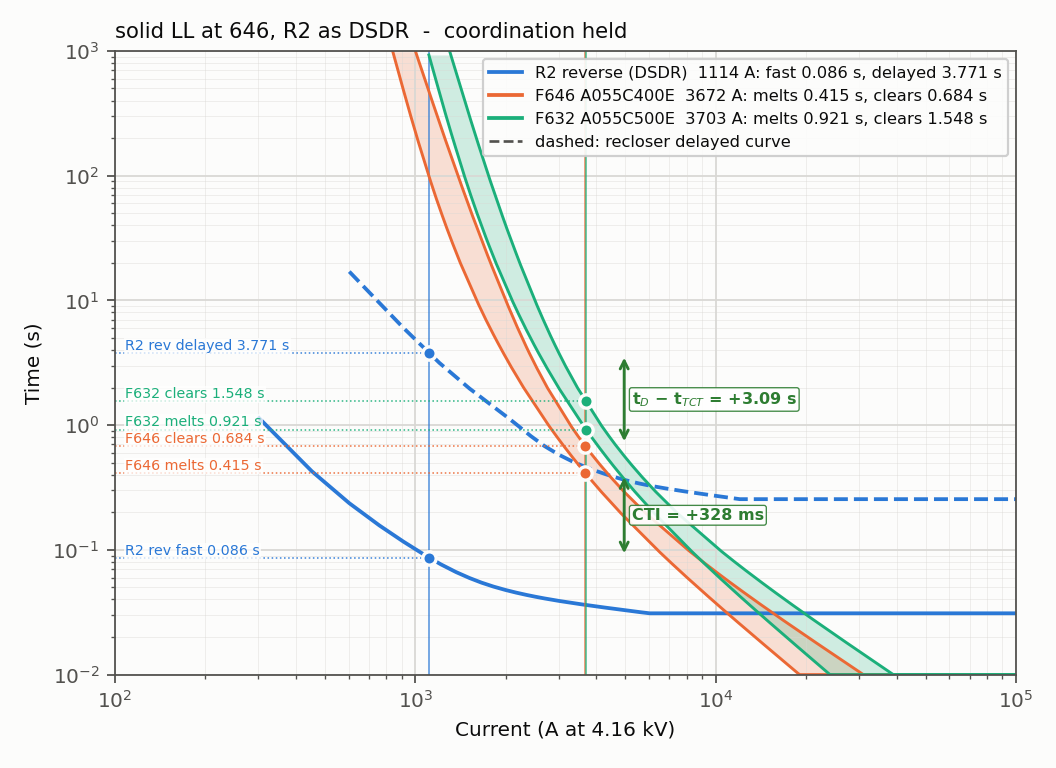
\includegraphics[width=0.68\textwidth]{fig15.png}
\caption{Bolted LL fault at 646: R2 reverse setting with F646 and F632; CTI = +328\,ms.}
\label{fig:f15}
\end{figure}

\begin{figure}[H]
\centering
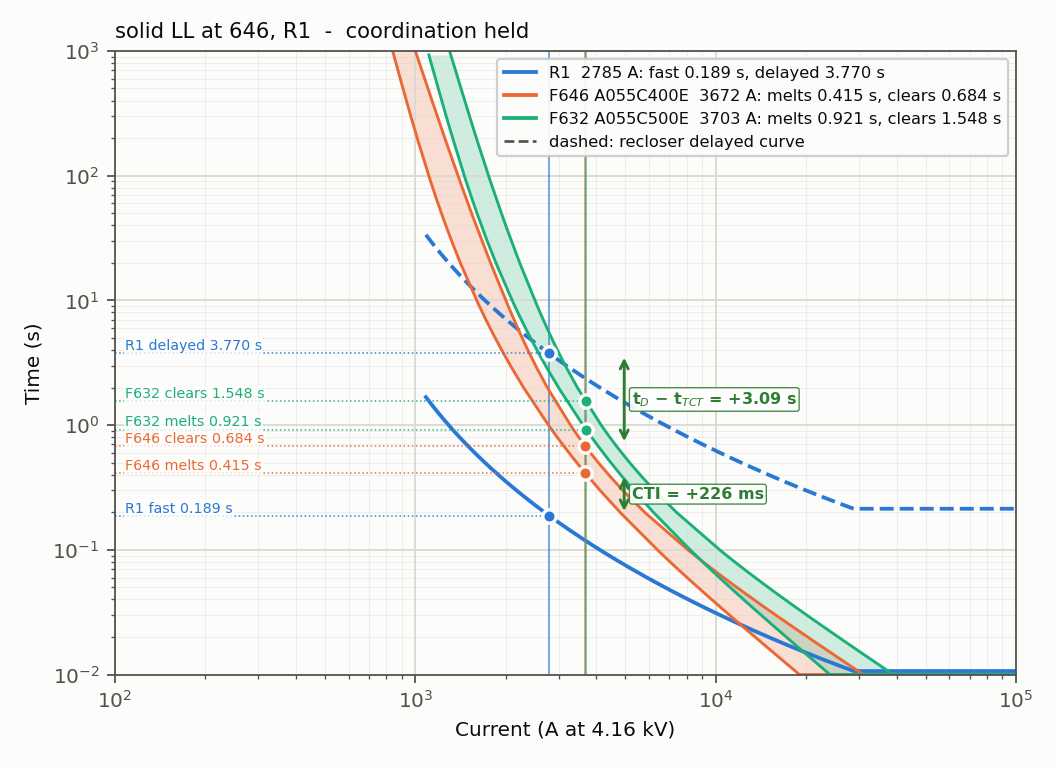
\includegraphics[width=0.68\textwidth]{fig16.png}
\caption{Bolted LL fault at 646: R1 with F646 and F632; CTI = +226\,ms.}
\label{fig:f16}
\end{figure}

\subsection{Operating Times With the DSDR}
Tables~\ref{tab:t4a} and \ref{tab:t4b} give the operating times with the DSDR. R1 operates forward for every node.
R2 operates in reverse for the nodes upstream of it and forward for the nodes downstream. The fuse time is
the minimum-melting time of the fuse nearest to the fault at the current through that fuse. In all nine
rows with a fuse it is longer than the last fast trip; the smallest margins are 6\,ms at 675 and 15\,ms at DL
and 652.

\begin{table}[H]
\centering\footnotesize
\setlength{\tabcolsep}{4pt}
\begin{tabular}{|l|l|c|c|c|c|c|c|c|}
\hline
 & & \textbf{$I_{R1}$} & \textbf{R1 fast} & \textbf{R1 delayed} & \textbf{$I_{R2}$} & & \textbf{R2 fast} & \textbf{R2 delayed} \\
\textbf{Node} & \textbf{Fault} & \textbf{(A)} & \textbf{(s)} & \textbf{(s)} & \textbf{(A)} & \textbf{Dir.} & \textbf{(s)} & \textbf{(s)} \\ \hline
632 & LLL & 4734 & 0.081 & 1.627 & 1813 & rev & 0.051 & 1.416 \\ \hline
633 & LLL & 3970 & 0.106 & 2.111 & 1500 & rev & 0.060 & 2.001 \\ \hline
645 & LL & 3124 & 0.155 & 3.095 & 1232 & rev & 0.075 & 3.002 \\ \hline
646 & LL & 2785 & 0.189 & 3.770 & 1114 & rev & 0.086 & 3.771 \\ \hline
DL & LLL & 3954 & 0.106 & 2.123 & 1972 & rev & 0.048 & 1.213 \\ \hline
671 & LLL & 3412 & 0.134 & 2.677 & 3391 & fwd & 0.054 & 1.600 \\ \hline
692 & LLL & 3412 & 0.134 & 2.677 & 3391 & fwd & 0.054 & 1.600 \\ \hline
675 & LLL & 3090 & 0.158 & 3.152 & 3050 & fwd & 0.059 & 1.941 \\ \hline
684 & LL & 2543 & 0.222 & 4.437 & 2543 & fwd & 0.072 & 2.813 \\ \hline
680 & LLL & 2789 & 0.188 & 3.761 & 2757 & fwd & 0.066 & 2.381 \\ \hline
611 & LG & 1814 & 0.435 & 8.709 & 1718 & fwd & 0.128 & 6.986 \\ \hline
652 & LG & 1795 & 0.446 & 8.919 & 1761 & fwd & 0.123 & 6.570 \\ \hline
\end{tabular}
\caption{Recloser operating times with the DSDR, DG in service.}
\label{tab:t4a}
\end{table}

\begin{table}[H]
\centering\footnotesize
\setlength{\tabcolsep}{4pt}
\begin{tabular}{|l|l|l|c|c|c|c|c|c|l|}
\hline
 & & & & \textbf{$I_{fuse}$} & \textbf{$t_{MMT}$} & \textbf{$t_{TCT}$} & \textbf{Last fast} & \textbf{Margin} & \\
\textbf{Node} & \textbf{Fault} & \textbf{Fuse} & \textbf{Size} & \textbf{(A)} & \textbf{(s)} & \textbf{(s)} & \textbf{trip (s)} & \textbf{(s)} & \textbf{Status} \\ \hline
633 & LLL & F633 & 400E & 5426 & 0.149 & 0.235 & 0.106 & $+0.043$ & held \\ \hline
645 & LL & F632 & 500E & 4191 & 0.613 & 0.970 & 0.155 & $+0.458$ & held \\ \hline
646 & LL & F646 & 400E & 3672 & 0.415 & 0.684 & 0.189 & $+0.226$ & held \\ \hline
DL & LLL & F-DL & 400E & 5902 & 0.121 & 0.193 & 0.106 & $+0.015$ & held \\ \hline
692 & LLL & F671-1 & 400E & 3391 & 0.525 & 0.891 & 0.054 & $+0.471$ & held \\ \hline
675 & LLL & F692-R & 250E & 5022 & 0.065 & 0.106 & 0.059 & $+0.006$ & held \\ \hline
684 & LL & F671-2 & 300E & 3963 & 0.148 & 0.230 & 0.072 & $+0.076$ & held \\ \hline
611 & LG & F684 & 200E & 2236 & 0.271 & 0.414 & 0.128 & $+0.143$ & held \\ \hline
652 & LG & F652 & 150E & 2239 & 0.138 & 0.193 & 0.123 & $+0.015$ & held \\ \hline
\end{tabular}
\caption{Fuse times with the DSDR, DG in service. Margin = $t_{MMT}$ minus the last fast trip (R2 for faults below R2; the later
of R1 and R2 reverse above it). Nodes 632, 671 and 680 are on the main feeder and have no fuse.}
\label{tab:t4b}
\end{table}

\subsection{Single Setting Against Dual Setting on Selected Faults}
Table~\ref{tab:cases9} compares the two settings of R2 on nine faults with the same (revised) fuses: the six
faults of the figures above and three cells of the classification.
Figures~\ref{fig:case5} and \ref{fig:case7} show two of the diagrams.

\begin{table}[H]
\centering\scriptsize
\setlength{\tabcolsep}{3pt}
\begin{tabularx}{\textwidth}{|c|l|L|c|c|c|c|c|c|c|l|l|}
\hline
 & & & \textbf{$Z_f$} & \textbf{$I_{R1}$} & \textbf{$I_{R2}$ (A),} & \textbf{R1 fast} & \multicolumn{2}{c|}{\textbf{R2 fast (s)}} & \textbf{Fuse: melts} & \multicolumn{2}{c|}{\textbf{Fuse saving}} \\
\textbf{\#} & \textbf{Figure} & \textbf{Fault} & \textbf{($\Omega$)} & \textbf{(A)} & \textbf{direction} & \textbf{(s)} & \textbf{single} & \textbf{dual} & \textbf{(s)} & \textbf{single} & \textbf{dual} \\ \hline
01 & Fig. 8 & LG fault at 611 & 0 & 1814 & 1718 (fwd) & 0.435 & 0.128 & 0.128 & F684 200E: 0.271 & held & held \\ \hline
02 & Fig. 9 & LLG fault at the middle of 692-675 & 1 & 1445 & 1310 (fwd) & 0.742 & 0.204 & 0.204 & F692-R 250E: 0.618 & held & held \\ \hline
03 & Fig. 11 & LL fault at 646 & 1 & 1899 & 847 (rev) & 0.395 & 0.500 & 0.131 & F646 400E: 1.734 & lost & lost \\ \hline
04 & Fig. 12 & LL fault at 645 & 1.5 & 1694 & 783 (rev) & 0.507 & 0.605 & 0.149 & F632 500E: 9.129 & lost & lost \\ \hline
05 & Fig. 13 & Three-phase fault at 10 \% of 632-633 & 0 & 4645 & 1777 (rev) & 0.084 & 0.121 & 0.052 & F633 400E: 0.100 & lost & held \\ \hline
06 & Figs. 15, 16 & LL fault at 646 & 0 & 2785 & 1114 (rev) & 0.189 & 0.278 & 0.086 & F646 400E: 0.415 & held & held \\ \hline
07 & Fig. 14 / 17 cell & LG fault at 646 (phase c) & 0 & 2359 & 469 (rev) & 0.255 & no trip & 0.396 & F646 400E: 1.057 & lost & held \\ \hline
08 & Fig. 14 / 17 cell & LG fault at 633 (phase b) & 0 & 2874 & 644 (rev) & 0.178 & 0.974 & 0.210 & F633 400E: 0.502 & lost & held \\ \hline
09 & Fig. 14 / 17 cell & LG fault at 692 (phase a) & 0 & 2197 & 2182 (fwd) & 0.293 & 0.089 & 0.089 & F671-1 400E: 2.842 & lost & lost \\ \hline
\end{tabularx}
\caption{Nine faults with the DG in service: single-setting against dual-setting R2, same fuses.}
\label{tab:cases9}
\end{table}

In cases 5, 7 and 8 the dual setting restores the fuse saving: the reverse group picks up a DG current that
the forward group does not see (case 7: 469\,A) or sees only slowly. Cases 3, 4 and 9 are lost with both
settings; they are limits of the fuse revision and of the dial range, not of the direction. Cases 3 and 4 are
faults through impedance: the larger fuses that are needed for the bolted faults are too slow for
these lower currents. Cases 5 and 7 are shown in detail in Figures~\ref{fig:case5} and \ref{fig:case7};
Tables~\ref{tab:case5} and \ref{tab:case7} list their currents, settings and operating times.

\begin{figure}[H]
\centering
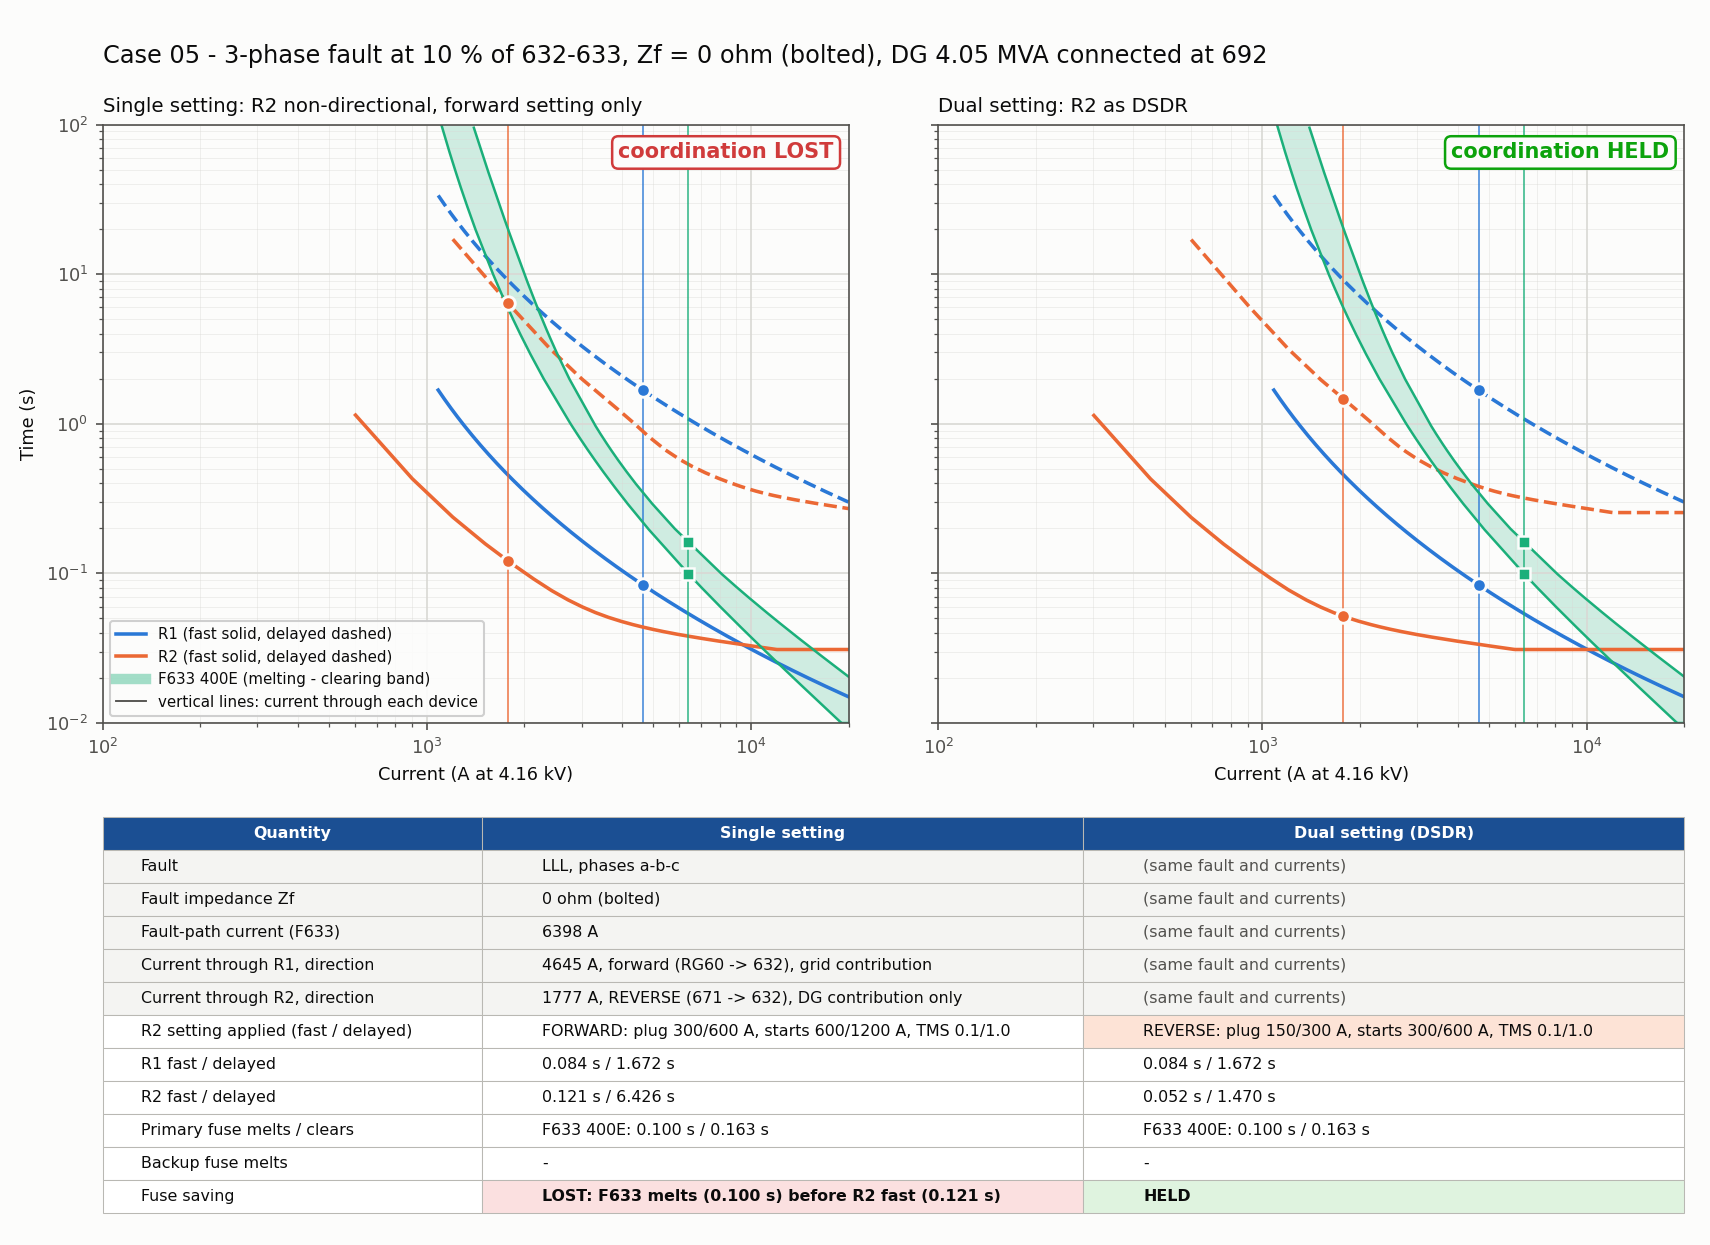
\includegraphics[width=\textwidth]{case05.png}
\caption{Three-phase fault at 10 per cent of line 632--633: single setting (left, CTI = $-22$\,ms) and dual setting
(right, CTI = +16\,ms).}
\label{fig:case5}
\end{figure}

\begin{table}[H]
\centering
\footnotesize
\setlength{\tabcolsep}{4pt}
\begin{tabularx}{\textwidth}{|p{4.4cm}|L|L|}
\hline
\textbf{Quantity} & \textbf{Single setting} & \textbf{Dual setting (DSDR)} \\ \hline
Fault & \multicolumn{2}{l|}{Three-phase fault at 10 \% of 632-633, LLL, phases a-b-c} \\ \hline
Fault impedance $Z_f$ & \multicolumn{2}{l|}{0\ohm{} (bolted)} \\ \hline
Fault-path current (F633) & \multicolumn{2}{l|}{6398 A} \\ \hline
Current through R1, direction & \multicolumn{2}{l|}{4645 A, forward (RG60 $\rightarrow$ 632), grid contribution} \\ \hline
Current through R2, direction & \multicolumn{2}{l|}{1777 A, REVERSE (671 $\rightarrow$ 632), DG contribution only} \\ \hline
R2 setting applied (fast / delayed) & FORWARD: plug 300/600 A, starts 600/1200 A, TMS 0.1/1.0 & REVERSE: plug 150/300 A, starts 300/600 A, TMS 0.1/1.0 \\ \hline
R1 fast / delayed & 0.084 s / 1.672 s & 0.084 s / 1.672 s \\ \hline
R2 fast / delayed & 0.121 s / 6.426 s & 0.052 s / 1.470 s \\ \hline
Primary fuse melts / clears & F633 400E: 0.100 s / 0.163 s & F633 400E: 0.100 s / 0.163 s \\ \hline
Backup fuse melts & - & - \\ \hline
Fuse saving & LOST: F633 melts (0.100 s) before R2 fast (0.121 s) & HELD \\ \hline
\end{tabularx}
\caption{Three-phase fault at 10 per cent of line 632--633: currents, settings and operating times.}
\label{tab:case5}
\end{table}

\begin{figure}[H]
\centering
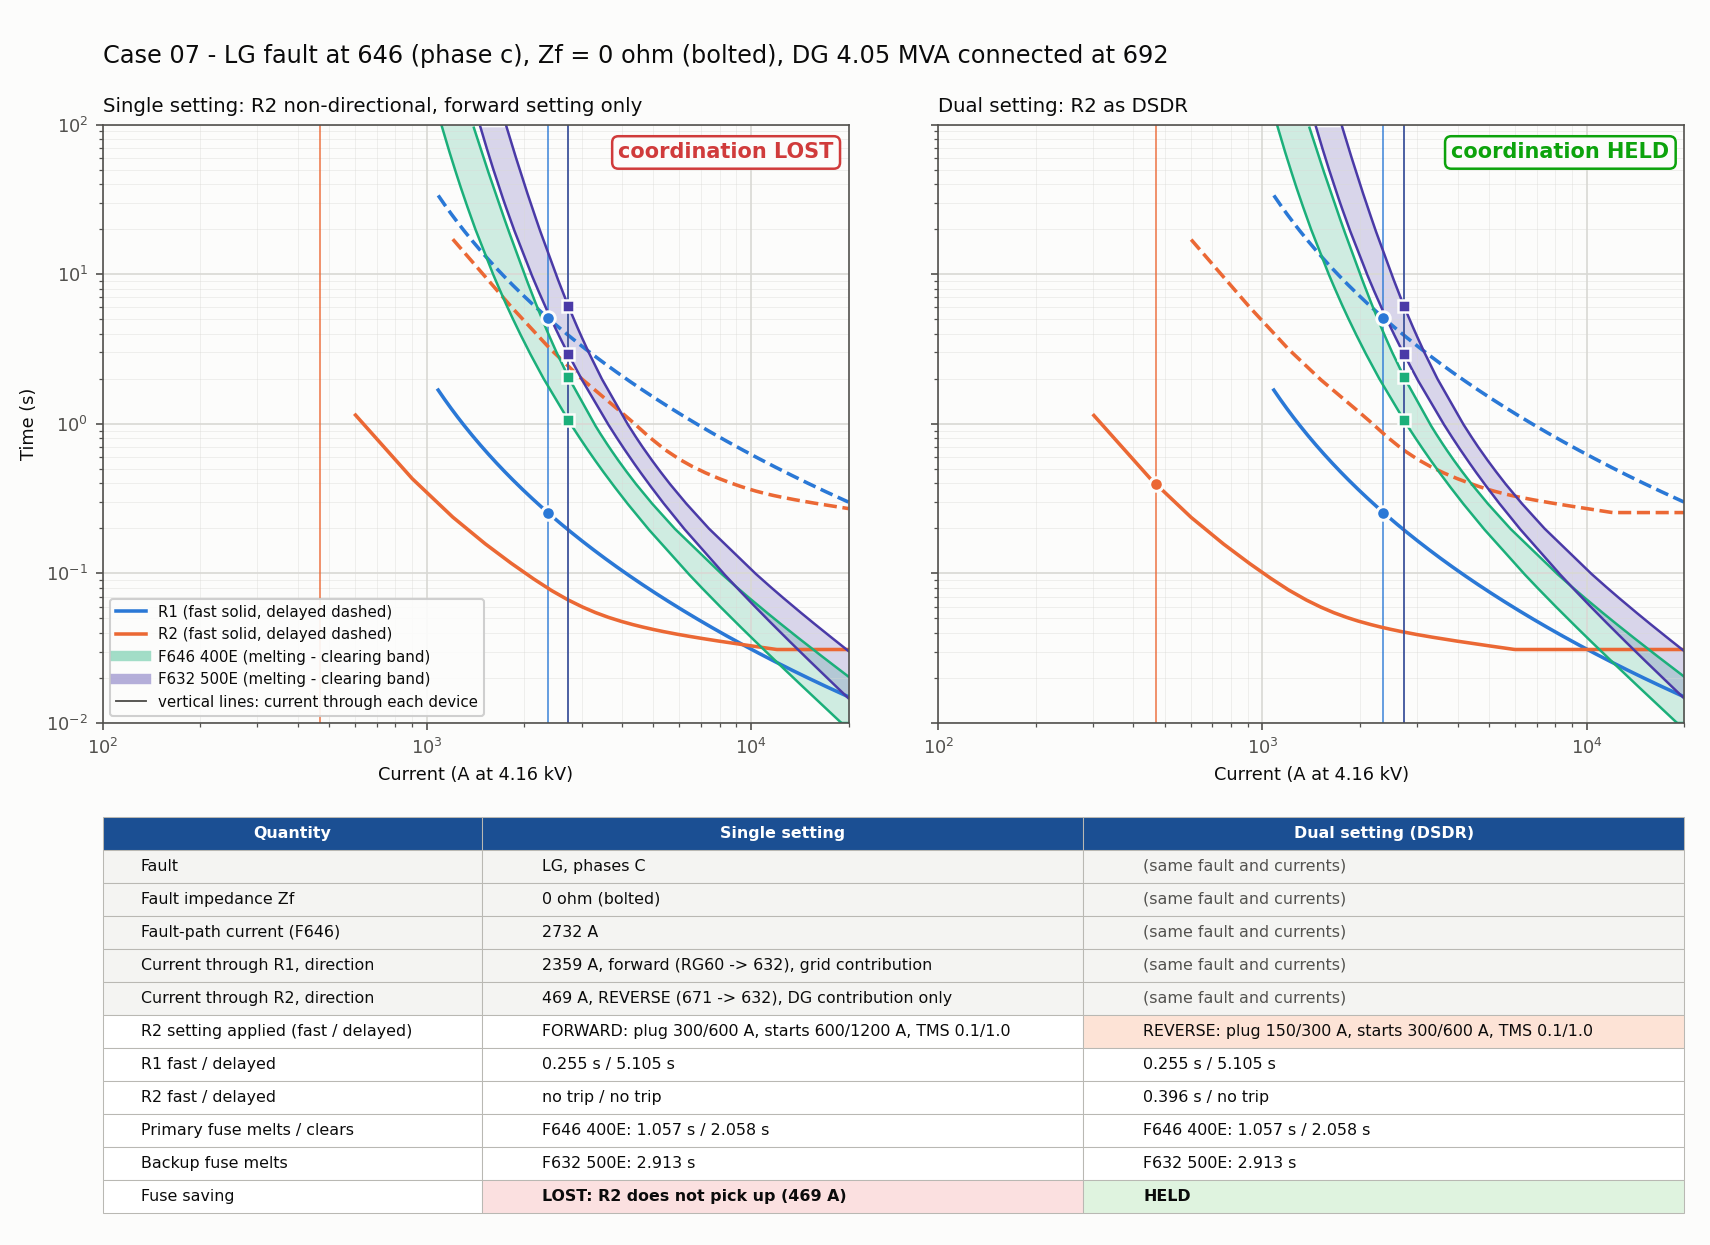
\includegraphics[width=\textwidth]{case07.png}
\caption{LG fault at 646: the single-setting R2 does not pick up the reverse current (left); the reverse group
does (right, CTI = +661\,ms).}
\label{fig:case7}
\end{figure}

\begin{table}[H]
\centering
\footnotesize
\setlength{\tabcolsep}{4pt}
\begin{tabularx}{\textwidth}{|p{4.4cm}|L|L|}
\hline
\textbf{Quantity} & \textbf{Single setting} & \textbf{Dual setting (DSDR)} \\ \hline
Fault & \multicolumn{2}{l|}{LG fault at 646 (phase c), LG, phases C} \\ \hline
Fault impedance $Z_f$ & \multicolumn{2}{l|}{0\ohm{} (bolted)} \\ \hline
Fault-path current (F646) & \multicolumn{2}{l|}{2732 A} \\ \hline
Current through R1, direction & \multicolumn{2}{l|}{2359 A, forward (RG60 $\rightarrow$ 632), grid contribution} \\ \hline
Current through R2, direction & \multicolumn{2}{l|}{469 A, REVERSE (671 $\rightarrow$ 632), DG contribution only} \\ \hline
R2 setting applied (fast / delayed) & FORWARD: plug 300/600 A, starts 600/1200 A, TMS 0.1/1.0 & REVERSE: plug 150/300 A, starts 300/600 A, TMS 0.1/1.0 \\ \hline
R1 fast / delayed & 0.255 s / 5.105 s & 0.255 s / 5.105 s \\ \hline
R2 fast / delayed & no trip / no trip & 0.396 s / no trip \\ \hline
Primary fuse melts / clears & F646 400E: 1.057 s / 2.058 s & F646 400E: 1.057 s / 2.058 s \\ \hline
Backup fuse melts & F632 500E: 2.913 s & F632 500E: 2.913 s \\ \hline
Fuse saving & LOST: R2 does not pick up (469 A) & HELD \\ \hline
\end{tabularx}
\caption{LG fault at 646 (phase c): currents, settings and operating times.}
\label{tab:case7}
\end{table}

\subsection{Time-Sequence Check}
The classification above uses the strict rule that every recloser must trip before the fuse starts to melt.
A time-sequence check follows each fault in time instead: the fuse heats with the current that still flows
after each recloser opens. For the 18 cells upstream of R2 the strict rule gives 11 cells held with the single
setting and 18 with the dual setting; the time sequence gives 15 and 18 (Figure~\ref{fig:seq}). The three
cells that the DSDR restores in the time sequence as well are the LG faults at 633, 645 and 646, where the
single-setting R2 never trips on a reverse current of about 0.5 to 0.6\,kA. For the 21 cells downstream of R2 the DG
at 692 feeds the fault directly, with no recloser in its path, and the result is the same for both settings.

\begin{figure}[H]
\centering
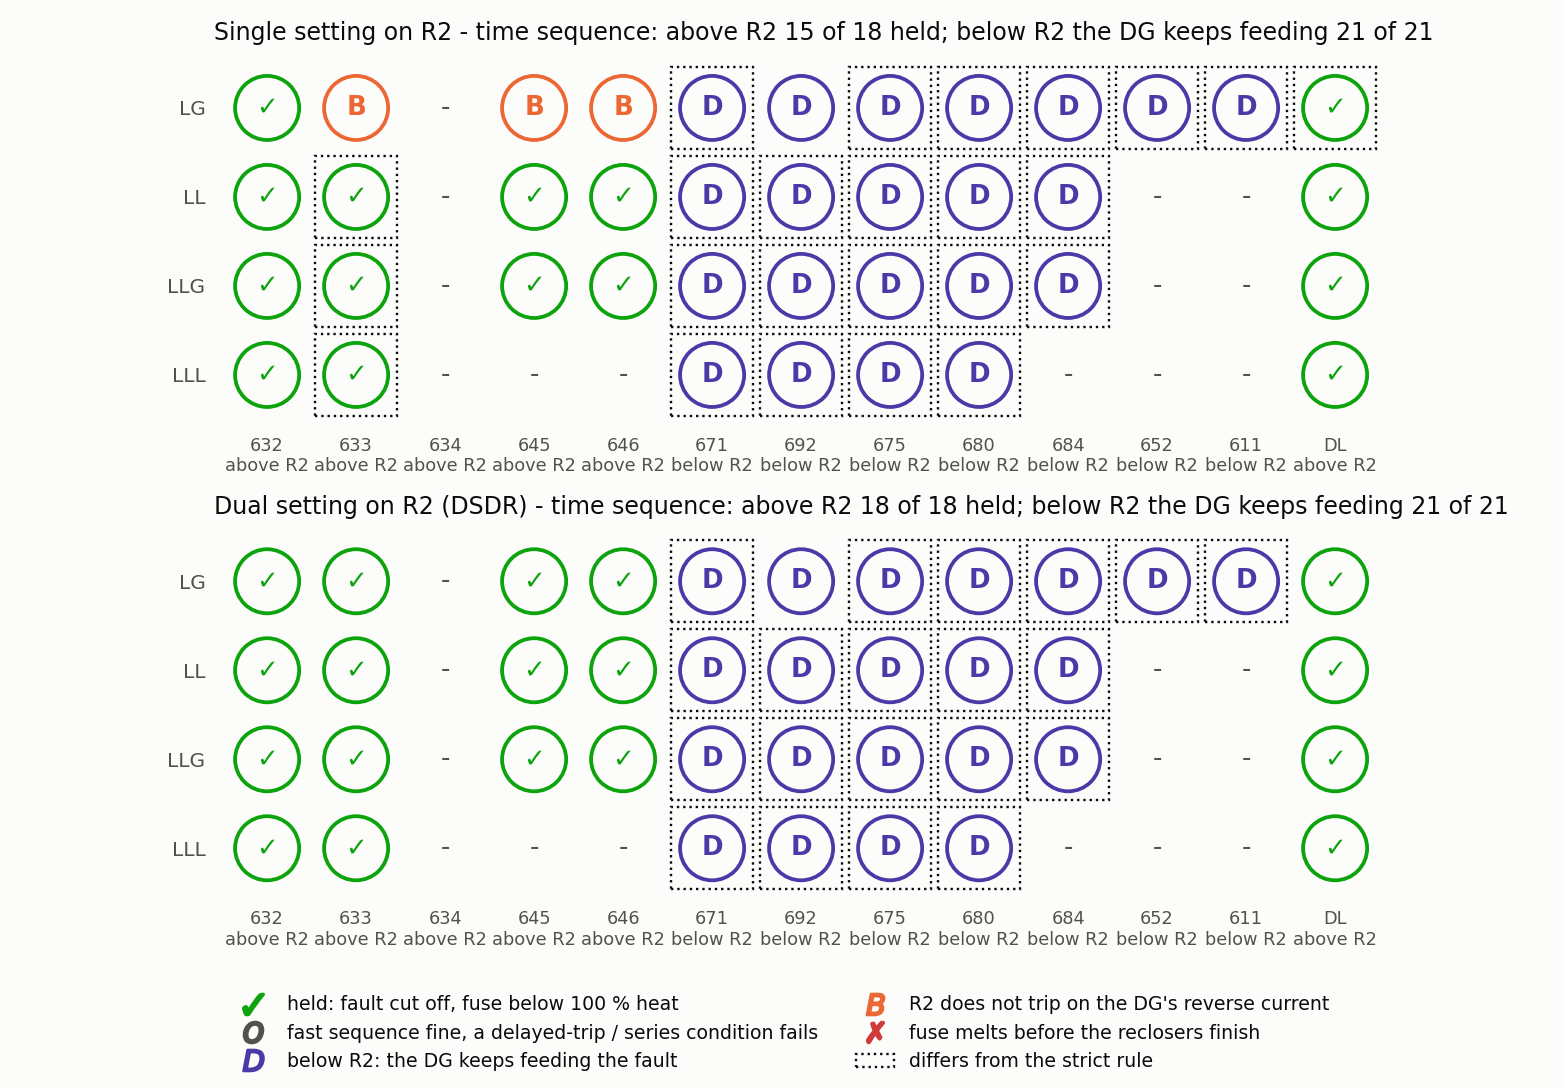
\includegraphics[width=\textwidth]{cd_sequence.png}
\caption{Time-sequence check of all 39 cells, single against dual setting.}
\label{fig:seq}
\end{figure}

\subsection{Time-Domain Verification}
Figure~\ref{fig:f10} is the EMT simulation of an LL (a--c) fault at 684 through 0.2\ohm{} with the
conventional settings. The recloser trips follow R2's fast curve applied to the simulated current,
and the fuse F671-2 (300E) melts when the accumulated heating $\sum \Delta t / t_{MMT}(I)$ reaches one.
Without DG the two fast shots use 45 per cent of the melting heat, the fuse survives both and then clears the
permanent fault. With the DG the fuse melts at the end of the second fast shot, because the DG keeps feeding
the fault while R2 is open (Table~\ref{tab:emt}). The feeder current at node 632 is 557 / 588\,A RMS
(phases a / c) before the fault and 2362 / 2719\,A during it, with peaks of 3338 / 3842\,A.

\begin{figure}[H]
\centering
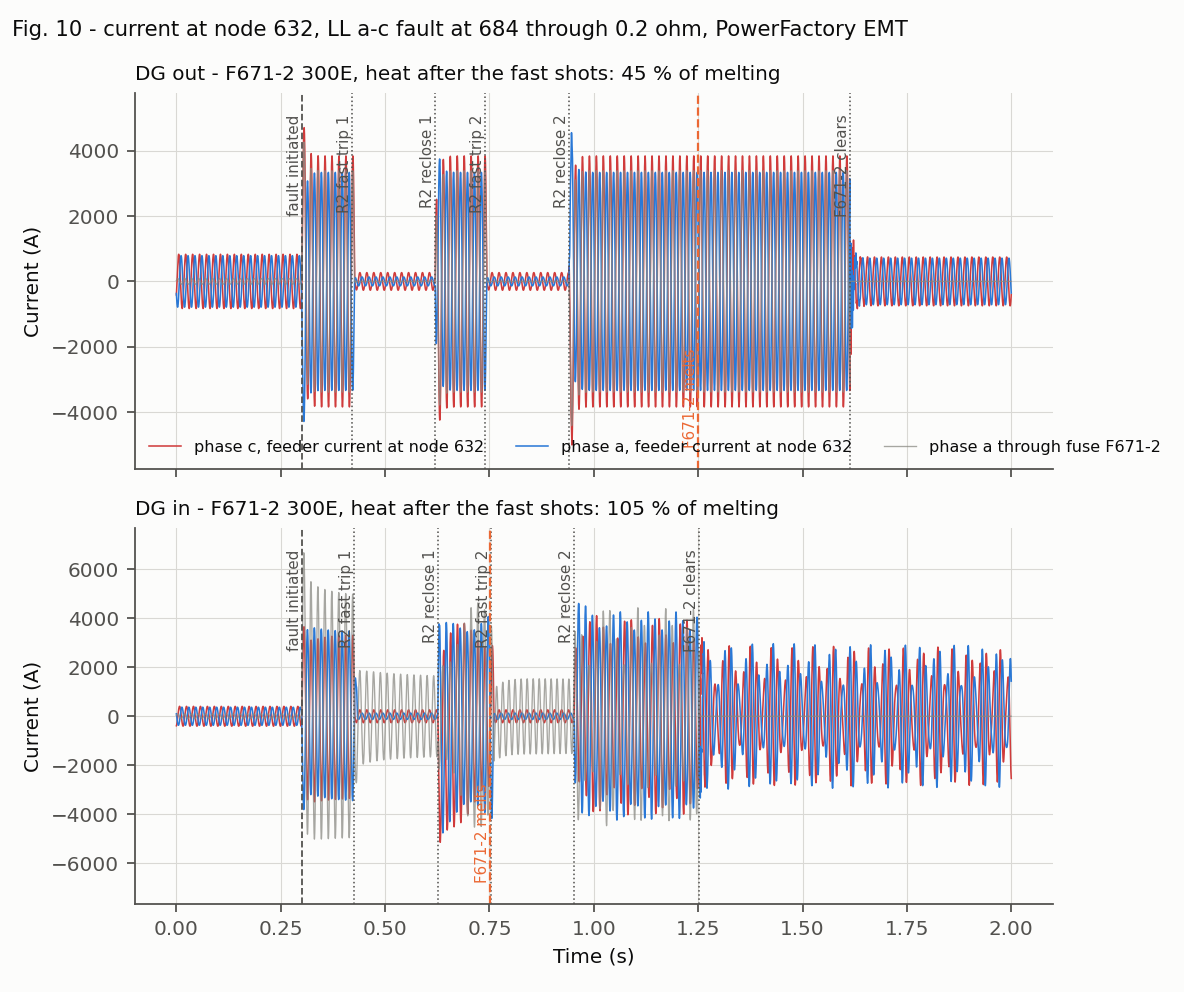
\includegraphics[width=0.95\textwidth]{fig10.png}
\caption{Time-domain current at node 632 for an LL (a--c) fault at 684 through 0.2\ohm{} :
without DG (top) and with DG (bottom).}
\label{fig:f10}
\end{figure}

\begin{table}[H]
\centering\small
\begin{tabular}{|l|c|c|}
\hline
\textbf{Event (time in s)} & \textbf{DG out} & \textbf{DG in} \\ \hline
Fault initiated & 0.30 & 0.30 \\ \hline
R2 fast trip 1 & 0.420 & 0.426 \\ \hline
R2 reclose 1 & 0.620 & 0.626 \\ \hline
R2 fast trip 2 & 0.740 & 0.753 \\ \hline
R2 reclose 2 & 0.940 & 0.953 \\ \hline
Fuse F671-2 melts & 1.248 & 0.752 \\ \hline
Fuse operation / clears & 1.613 & 1.253 \\ \hline
Fuse heat after the fast shots & 45\,\% & 105\,\% \\ \hline
\end{tabular}
\caption{Reclosing sequence of the EMT simulation.}
\label{tab:emt}
\end{table}

\subsection{Verification With the Relay and Fuse Models of \PF}
The operating times of Chapter Five are calculated from the time--current curves of the devices. As a check,
the settings were entered into the relay and fuse elements of the model, and \PF{} itself calculated the tripping
time of every device for every fault, for the conventional and for the DSDR settings.

\subsection{Sensitivity of the Pickups With DG}
\label{sec:pickdg}
The pickups are a further limit of the settings. With the DG, the lowest LG fault current through 3\ohm{} is
577\,A at R1 and 368\,A at R2, below the pickups of 734.6\,A and 587.5\,A, because the DG supplies part of
the fault.

\subsection{Effect of the DG Penetration Level}
\label{sec:pen}
To see how the conventional coordination degrades as the DG grows, seven separate \PF{} projects were made,
copies of the model with the DG at 692 set to 0, 10, 25, 37, 50, 75 and 100 per cent of 4.05\,MVA. The machine, its
step-up transformer and its active and reactive power are scaled together, so the per-unit data of
Table~\ref{tab:dg} stay the same; at 0 per cent the DG is out of service. Every model keeps the conventional
protection of the design without DG (single-setting R2, fuses of the design without DG), and all operating
times are \PF's own relay and fuse calculations. Two fuse--recloser pairs are followed: fuse F633 against R1
for a three-phase fault at 633 (R1's zone), and the lateral fuse F671-2 at node 671 against R2 for a
line-to-line fault at 684 (R2's zone). The coordination time interval is
\begin{equation}
CTI = t_{MMT}(\text{fuse}) - t_{F}(\text{recloser}),
\label{eq:cti}
\end{equation}
and, for the doughnut chart of Figure~\ref{fig:penring}, each level's share of the ring,
$CTI\,\% = 100 \times CTI / \sum |CTI|$ over the seven levels, so that each ring adds up to 100 per cent.

\begin{table}[H]
\centering\scriptsize
\setlength{\tabcolsep}{3.2pt}
\begin{tabular}{|c|c|c|c|c|c|c|c|c|c|}
\hline
 & & \multicolumn{4}{c|}{\textbf{Node 633: F633 and R1 (LLL)}} & \multicolumn{4}{c|}{\textbf{Node 671: F671-2 and R2 (LL at 684)}} \\
\textbf{DG (\%)} & \textbf{MVA} & \textbf{$I$ fuse / R1 (A)} & \textbf{$t_{MMT}$ / $t_F$ (s)} & \textbf{CTI (ms)} & \textbf{ring \%} &
\textbf{$I$ fuse / R2 (A)} & \textbf{$t_{MMT}$ / $t_F$ (s)} & \textbf{CTI (ms)} & \textbf{ring \%} \\ \hline
0 & 0.00 & 4102 / 4162 & 0.102 / 0.098 & $+4$ & $+2.1$ & 2574 / 2711 & 0.470 / 0.067 & $+403$ & $+26.0$ \\ \hline
10 & 0.41 & 4256 / 4142 & 0.094 / 0.099 & $-5$ & $-3.1$ & 2715 / 2681 & 0.401 / 0.068 & $+333$ & $+21.5$ \\ \hline
25 & 1.01 & 4478 / 4111 & 0.083 / 0.100 & $-17$ & $-9.6$ & 2926 / 2636 & 0.323 / 0.069 & $+254$ & $+16.4$ \\ \hline
37 & 1.50 & 4648 / 4088 & 0.077 / 0.101 & $-24$ & $-13.9$ & 3094 / 2598 & 0.277 / 0.070 & $+207$ & $+13.4$ \\ \hline
50 & 2.02 & 4824 / 4062 & 0.071 / 0.102 & $-31$ & $-17.9$ & 3276 / 2557 & 0.237 / 0.072 & $+166$ & $+10.7$ \\ \hline
75 & 3.04 & 5140 / 4015 & 0.062 / 0.104 & $-42$ & $-24.2$ & 3623 / 2511 & 0.184 / 0.073 & $+110$ & $+7.1$ \\ \hline
100 & 4.05 & 5426 / 3970 & 0.055 / 0.106 & $-51$ & $-29.2$ & 3963 / 2543 & 0.147 / 0.072 & $+75$ & $+4.9$ \\ \hline
\end{tabular}
\caption{CTI against DG penetration, conventional protection.}
\label{tab:pencti}
\end{table}

\begin{figure}[H]
\centering
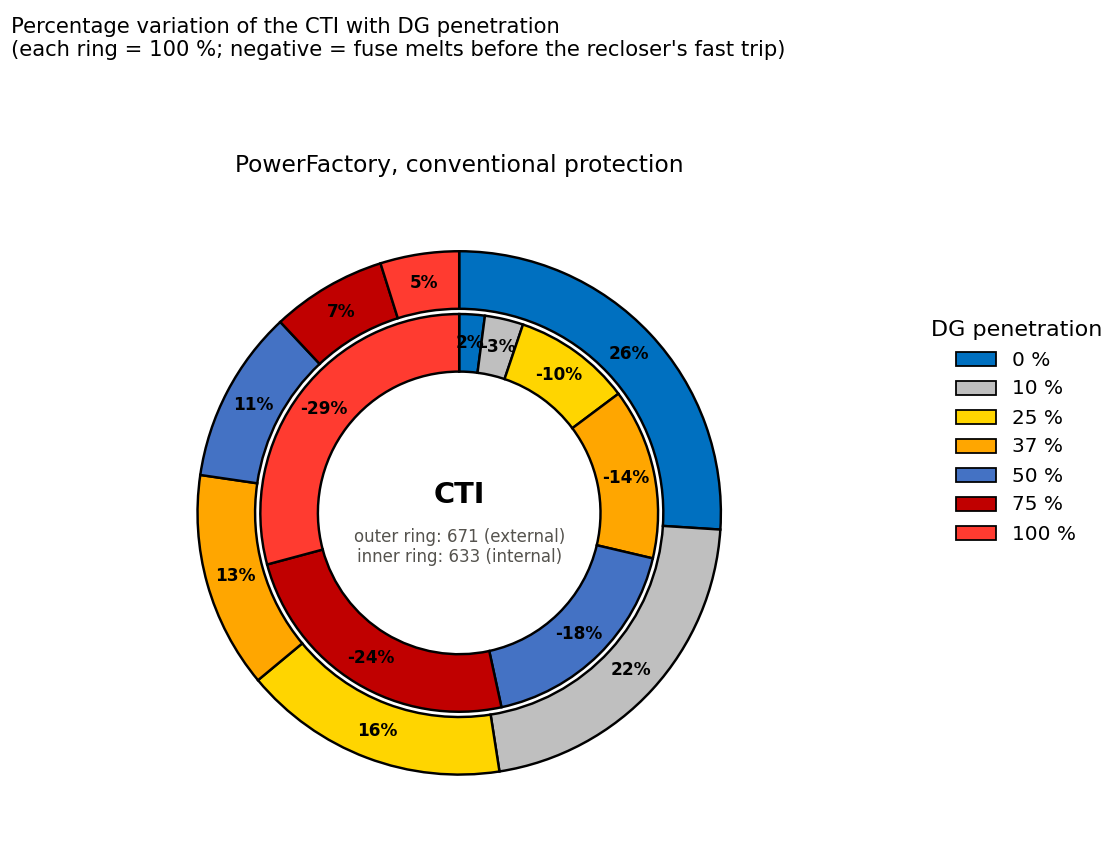
\includegraphics[width=0.62\textwidth]{pen_ring.png}
\caption{Percentage variation of the CTI with DG penetration (outer ring 671, inner ring 633).}
\label{fig:penring}
\end{figure}

At node 633 the fuse current rises from 4102\,A to 5426\,A while R1's current falls from 4162\,A to 3970\,A; the CTI falls from $+4$\,ms to $-51$\,ms. At node 671 the fuse current rises from 2574\,A to 3963\,A while R2's current stays at about 2543\,A; the CTI falls from $+403$\,ms to $+75$\,ms. The mechanism is the same at both nodes
(Figure~\ref{fig:pencur}): the fuse lies between the fault and both sources and carries the grid share and
the DG share, while the recloser carries only the grid share, which even falls slightly because the DG holds
up the voltage of the network during the fault. A fuse curve is steep, so the extra current shortens its
melting time much more than the lower current lengthens the recloser's time, and the CTI decreases. At 633
the margin is only a few milliseconds without DG and is lost from about 4 per cent penetration; at 671 the margin
is large and stays positive up to 100 per cent.

\begin{figure}[H]
\centering
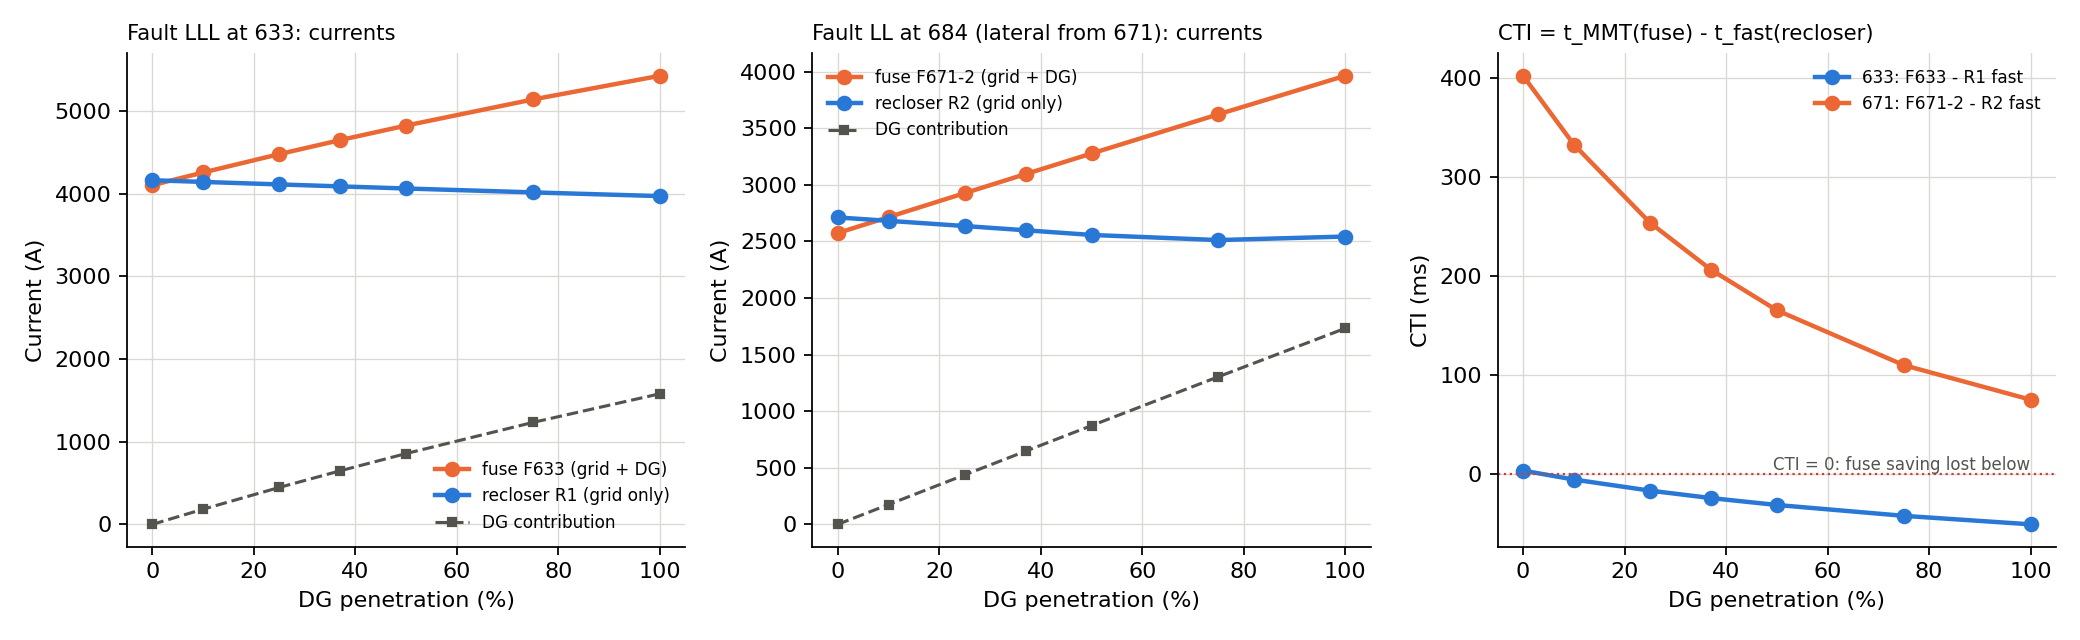
\includegraphics[width=\textwidth]{pen_currents.png}
\caption{Currents through the fuse (grid and DG share), the recloser (grid share) and from the DG, and the
resulting CTI, against DG penetration.}
\label{fig:pencur}
\end{figure}

Figure~\ref{fig:pentcc} shows the same on the time--current characteristics: the curves are fixed because
the settings are not changed, the recloser's operating point stays where it is, and the fuse's operating
point moves to a higher current and a shorter time with every step. Figure~\ref{fig:pentcc633} gives node 633
level by level, with the vertical short-circuit lines of the fuse and the recloser currents, the operating
times and the CTI.

\begin{figure}[H]
\centering
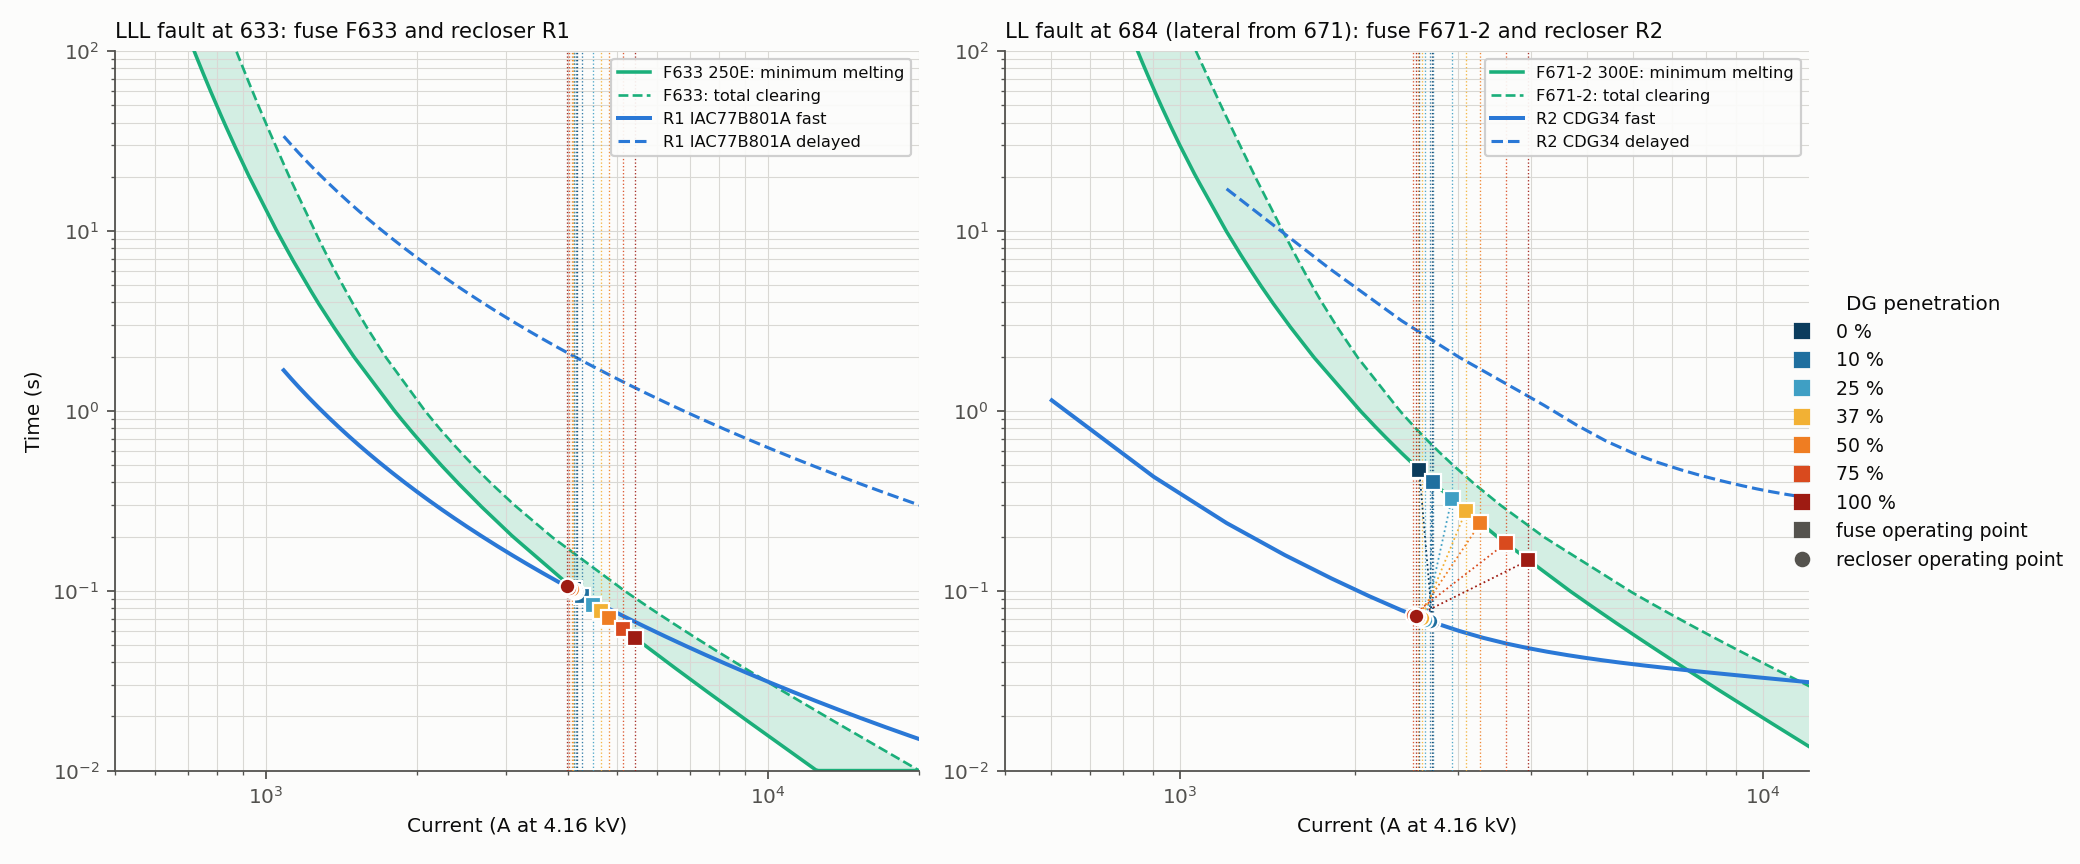
\includegraphics[width=\textwidth]{pen_tcc.png}
\caption{Time--current characteristics at all penetration levels: fuse operating points (squares) and recloser
operating points (circles).}
\label{fig:pentcc}
\end{figure}

\begin{figure}[H]
\centering
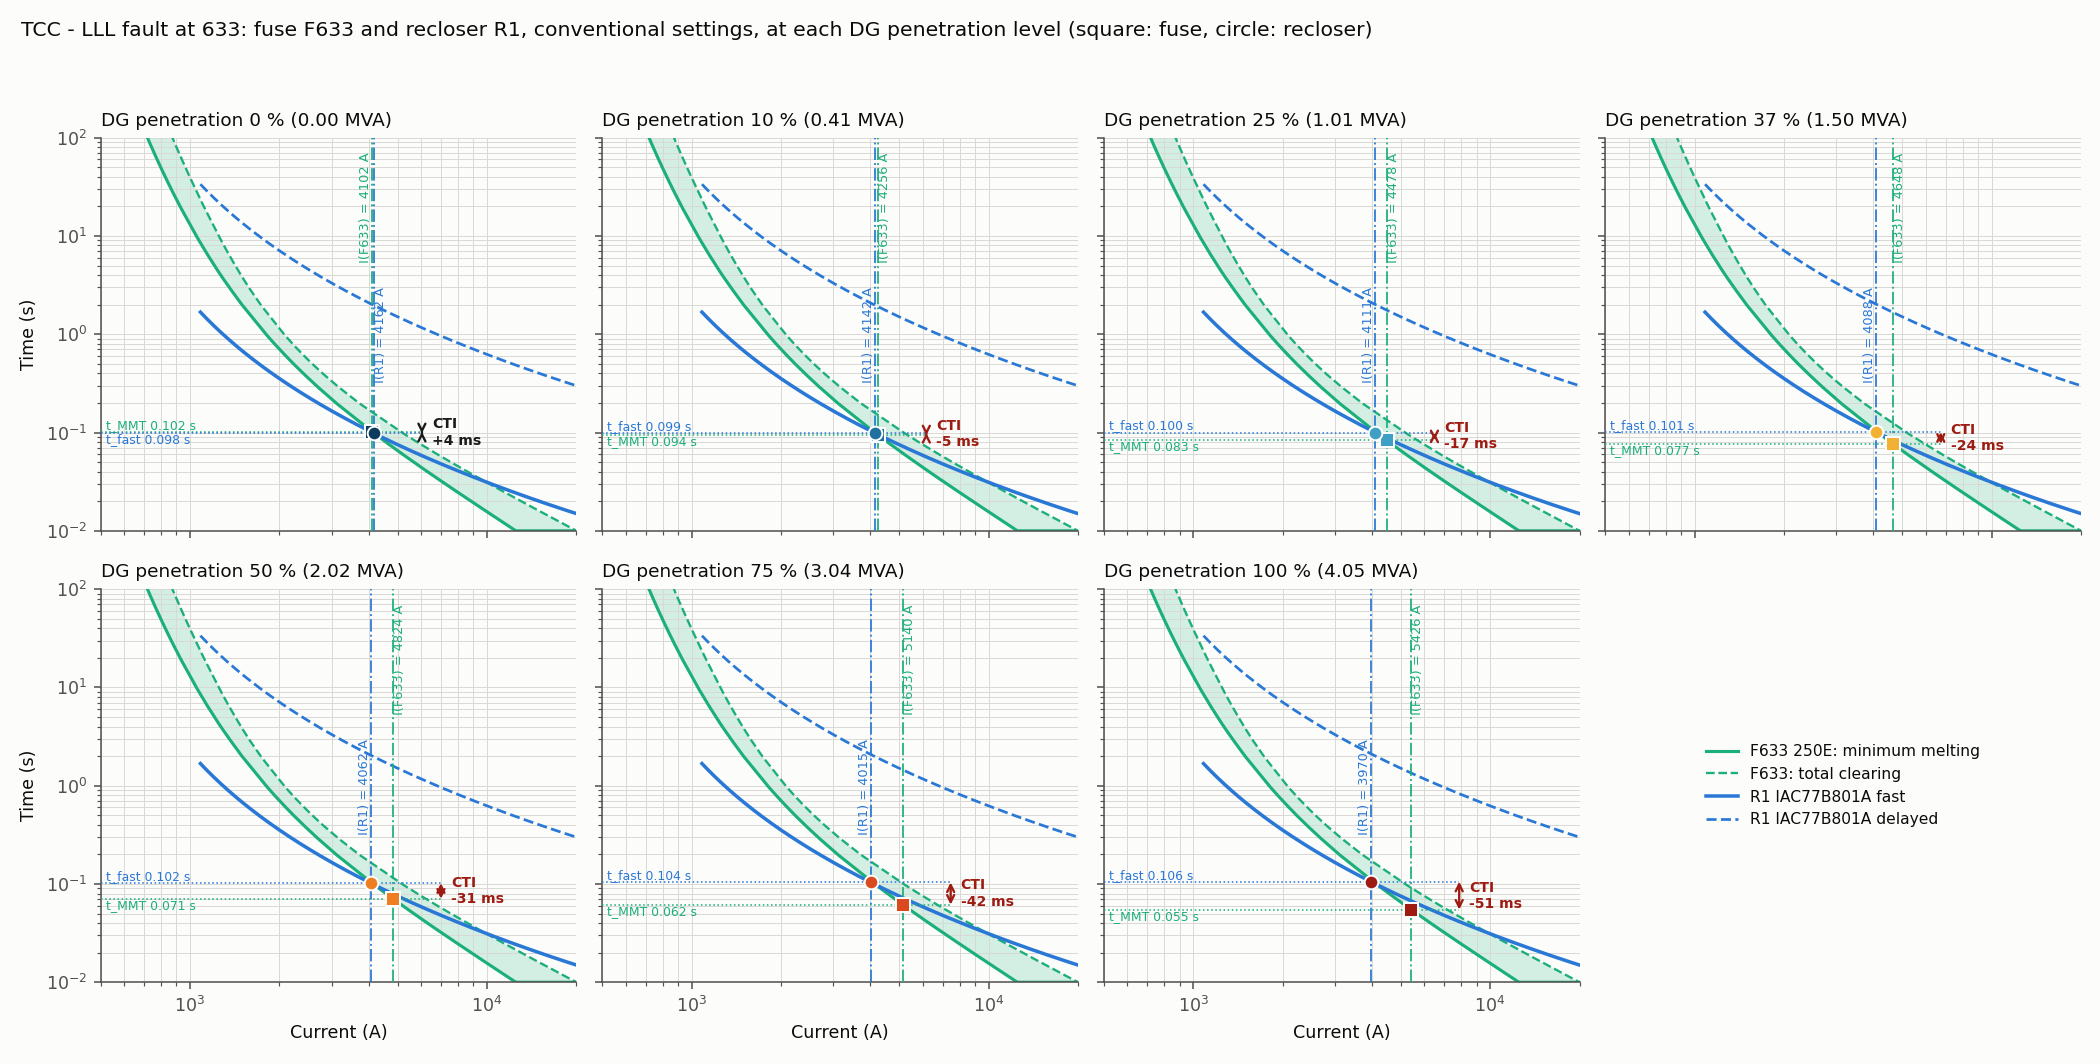
\includegraphics[width=\textwidth]{pen_tcc633.png}
\caption{Node 633, fuse F633 and R1, at each penetration level, with the short-circuit currents, operating times
and CTI.}
\label{fig:pentcc633}
\end{figure}

The fault level rises at every node (Table~\ref{tab:pensc}), most near the DG (671, 692, 675: about
$+60$ per cent) and least behind the 4.16/0.48\,kV transformer (634) and on the single-phase laterals. The current
through the reclosers does not rise with it.

\begin{table}[H]
\centering\footnotesize
\begin{tabular}{|l|l|c|c|c|c|c|c|}
\hline
\textbf{Node} & \textbf{Fault} & \textbf{0\,\%} & \textbf{25\,\%} & \textbf{50\,\%} & \textbf{75\,\%} & \textbf{100\,\%} & \textbf{Change} \\ \hline
632 & LLL ABC & 4735 & 5227 & 5690 & 6123 & 6526 & $+38\,\%$ \\ \hline
633 & LLL ABC & 4102 & 4478 & 4824 & 5140 & 5426 & $+32\,\%$ \\ \hline
634 & LLL ABC & 15671 & 16307 & 16828 & 17257 & 17608 & $+12\,\%$ \\ \hline
645 & LLG BC & 3418 & 3685 & 3932 & 4149 & 4341 & $+27\,\%$ \\ \hline
646 & LLG BC & 3112 & 3332 & 3528 & 3701 & 3854 & $+24\,\%$ \\ \hline
671 & LLL ABC & 3390 & 3919 & 4461 & 5010 & 5564 & $+64\,\%$ \\ \hline
692 & LLL ABC & 3390 & 3919 & 4461 & 5010 & 5564 & $+64\,\%$ \\ \hline
675 & LLL ABC & 3151 & 3612 & 4087 & 4557 & 5022 & $+59\,\%$ \\ \hline
680 & LLL ABC & 2930 & 3322 & 3711 & 4091 & 4460 & $+52\,\%$ \\ \hline
684 & LLG AC & 2655 & 3027 & 3395 & 3756 & 4107 & $+55\,\%$ \\ \hline
652 & LG A & 1874 & 1983 & 2080 & 2164 & 2239 & $+19\,\%$ \\ \hline
611 & LG C & 1857 & 1973 & 2074 & 2161 & 2236 & $+20\,\%$ \\ \hline
DL & LLL ABC & 3946 & 4454 & 4952 & 5436 & 5902 & $+50\,\%$ \\ \hline
\end{tabular}
\caption{Largest bolted fault current at each node (A) against DG penetration.}
\label{tab:pensc}
\end{table}

The load flow changes as well (Table~\ref{tab:penlf}). The DG supplies part of the load locally, so the load
current through both reclosers falls, the voltages rise, and the power through R2 reverses between 75 and
100 per cent. By eq.~\eqref{eq:ipfw} the pickups would have to fall with the penetration; with the fixed settings
(R1 720\,A, its curve starting at 1080\,A; R2 fast curve starting at 600\,A) the reclosers no longer detect the
weakest faults (LG through 3\ohm) in their zones, R2 from just above 50 per cent.

\begin{table}[H]
\centering\scriptsize
\setlength{\tabcolsep}{3.5pt}
\begin{tabular}{|c|c|c|c|c|c|c|c|c|c|}
\hline
 & \textbf{DG P} & \textbf{R1 load} & \textbf{R2 load} & \textbf{R2} & \textbf{$V_{671,a}$} & \textbf{R1 $1.25\,I_{nom}$} & \textbf{R2 $1.25\,I_{nom}$} & \textbf{R1 lowest} & \textbf{R2 lowest} \\
\textbf{DG (\%)} & \textbf{(MW)} & \textbf{(A)} & \textbf{(A)} & \textbf{flow} & \textbf{(p.u.)} & \textbf{(A)} & \textbf{(A)} & \textbf{3\,$\Omega$ fault (A)} & \textbf{3\,$\Omega$ fault (A)} \\ \hline
0 & 0.00 & 587.7 & 470.0 & forward & 0.988 & 734.6 & 587.5 & 1074$^\ast$ & 878 \\ \hline
10 & 0.32 & 543.1 & 430.1 & forward & 0.994 & 678.9 & 537.6 & 1018$^\ast$ & 821 \\ \hline
25 & 0.81 & 480.7 & 372.2 & forward & 1.002 & 600.9 & 465.2 & 937$^\ast$ & 738 \\ \hline
37 & 1.20 & 434.8 & 328.6 & forward & 1.009 & 543.5 & 410.8 & 874$^\ast$ & 673 \\ \hline
50 & 1.62 & 389.9 & 285.3 & forward & 1.015 & 487.4 & 356.6 & 809$^\ast$ & 606 \\ \hline
75 & 2.43 & 321.2 & 222.4 & forward & 1.025 & 401.5 & 278.0 & 689$^\ast$ & 483$^\ast$ \\ \hline
100 & 3.24 & 284.9 & 252.2 & reverse & 1.033 & 356.1 & 315.2 & 577$^\ast$ & 368$^\ast$ \\ \hline
\end{tabular}
\caption{Load flow, pickups by eq.~\eqref{eq:ipfw} and lowest fault current through each recloser against DG penetration.
$^\ast$: below the start of the recloser's curve with the fixed settings (not detected).}
\label{tab:penlf}
\end{table}

The penetration study therefore shows the two ways in which fixed settings fail as the DG grows: the fuse
saving is lost because the fuse speeds up while the recloser does not, and the sensitivity is lost because
the currents through the reclosers fall. Both are reasons for settings that adapt to the DG, which is what
the dual-setting directional recloser provides.

\subsection{Results Summary}
\begin{table}[H]
\centering\small
\begin{tabularx}{\textwidth}{|L|c|}
\hline
\textbf{Stage} & \textbf{Cells held (of 39)} \\ \hline
A. No DG, starting fuse sizes & 35 \\ \hline
A. No DG, after the fuse revision (F692-R to 200E) & 39 \\ \hline
B. DG connected, conventional R2 & 24 \\ \hline
B. DG connected, no-DG fuses, R2 as DSDR & 25 \\ \hline
C. DG connected, revised fuses, conventional R2 & 31 \\ \hline
C. DG connected, revised fuses, R2 as DSDR & 38 \\ \hline
C. The same settings and fuses with the DG out of service & 37 \\ \hline
\end{tabularx}
\caption{Summary of the coordination results.}
\label{tab:summary}
\end{table}

The dual setting alone, with the fuses of the design without DG, restores one cell (24 to 25). Together with
the fuse revision it restores fourteen (24 to 38), seven of which need the dual setting.

% =====================================================================================================
% =====================================================================================================
\chapterhead{SIX}{DISCUSSION}

\subsection{Effect of DG on Fault Current}
The DG raises the fault current at every node, most near its connection point (671 and 692: from 3.39 to
5.56\,kA). The fuses carry this higher current and melt faster, while R1 carries about the same grid current
as before. The margin between the fuse and the fast trip, which is small even without DG, disappears.

\subsection{Effect of Fault Current Direction}
For faults at 632, 633, 645, 646 and DL the current through R2 is reverse and consists only of the DG
contribution. Its magnitude (0.5 to 2.0\,kA) is much lower than the forward fault currents for which the
forward group is set. A forward group with plugs of 300 and 600\,A responds slowly to these currents, or not
at all for LG faults.

\subsection{Performance of the Conventional Protection}
With the conventional single setting the scheme keeps coordination at the nodes on the main feeder and loses
it on the fused laterals of R1's zone and at 675. The loss depends on the location and on the fault type; it
is not a uniform failure of the feeder.

\subsection{Performance of the DSDR}
The reverse group, with half the plug settings, trips for every reverse fault before the fuse melts once the
fuses are revised. The result of 38 cells against 31 with the same fuses isolates its contribution. Without
the fuse revision the improvement is one cell only: at 633 and DL the fuses of the design without DG melt
in 0.05 to 0.16\,s with the DG, before R1's fast trip (0.11 to 0.18\,s), and no setting of R2 can change
R1's time. The
DSDR is therefore necessary but not sufficient.

\subsection{Limits Reached by the Devices}
R1's dials are the two extremes of the IAC range, and the CDG table ends at 0.1 and 1.0. The
method's dial revision has no room. The fuse revision creates a conflict between the two states of the
network: the larger fuses that are needed with the DG are too slow for two cells without it, and for the
faults through impedance. Fuse sizes cannot adapt to the DG state. For faults downstream of R2 the fuse
saving relies on the DG's own protection disconnecting it during the dead time, which is not part of the method.

\subsection{Engineering Implication}
Adaptive directional protection is justified where a DG is downstream of a mid-line recloser. To apply it,
the engineer must check the dial range of the actual relay, revise the fuse sizes for the DG state, verify the
pickup against the reduced minimum fault current with DG, and provide for the DG infeed to faults beyond the
recloser.

% =====================================================================================================
\chapterhead{SEVEN}{CONCLUSION AND FUTURE WORK}

\subsection{Conclusion}
The DSDR method of~\cite{yousaf2022} was implemented on the IEEE 13-node feeder in DIgSILENT \PF{} with
the manufacturer-based time--current characteristics of the protection devices. The feeder model agrees with the IEEE short-circuit
benchmark within about 2 per cent. Without DG, the revised fuse scheme achieves coordination in all
39 cells, compared with 35 of 39 cells with the starting fuse sizes. With the 4.05\,MVA DG at
node 692 and a conventional R2, coordination is held in 24 cells. The dual setting alone, with the
fuses of the design without DG, raises this to 25 cells; the fuse revision alone, with a single-setting R2,
to 31; and the two together to 38 of 39 cells. The combined DSDR and
fuse-revision strategy therefore substantially improves the coordination in the zone between the grid and
the DG, achieving 38 of 39 coordinated fault cells under the zero-margin criterion, and
seven of the restored cells need the dual setting. The remaining LG fault at node 692 is limited by the
maximum available R2 delayed dial.

The faults downstream of R2 with the DG in service remain outside what the dual setting can correct.

\subsection{Major Findings}
\begin{enumerate}
\item Fault levels at the IEEE 13-node benchmark (feeder head 4.73\,kA).
\item R1: pickup 720\,A, TDS 0.5 / 10, GE IAC extremely inverse curve.
\item R2 forward: plugs 300 / 600\,A, TMS 0.1 / 1.0; R2 reverse: plugs 150 / 300\,A, TMS 0.1 / 1.0; reverse
      pickup by eq.~\eqref{eq:iprv} 315.3\,A.
\item With DG the load current at R2 reverses (252\,A) and R2 carries 1.1 to 2.0\,kA in reverse for upstream
      faults.
\item Coordination (of 39 cells): 35 without DG with the starting fuses and 39 after the fuse revision;
      24 with DG and a conventional R2; 25 with the DSDR alone; 31 with the fuse revision
      alone; 38 with the DSDR and the fuse revision, under the zero-margin criterion.
\item The dual setting restores seven cells with the revised fuses and one cell without the revision.
\item The LG fault at 692 cannot be coordinated within the delayed dial range of R2.
\item With rising DG penetration and fixed settings the CTI falls at both studied nodes (633: from about
      $+4$ to $-51$\,ms; 671: from $+403$ to $+75$\,ms), the fault level rises by up to 64 per cent, and R2 stops
      detecting the weakest fault of its zone above about 50 per cent.
\item In the EMT simulation the fuse survives the two fast shots without DG and melts at 1.25\,s; with DG it melts during the second fast shot.
\end{enumerate}

\subsection{Contributions of the Present Work}
\begin{itemize}
\item A reproducible \PF{} implementation of the method: one command rebuilds the model and all results.
\item Separation of the effect of the dual setting from the effect of the fuse revision.
\item Identification of the limits of the method: dial range, DG-in against DG-out fuse sizes, DG infeed
      downstream of the recloser, and sensitivity of the pickups with DG.
\item A time-domain verification and a verification with the relay models of the tool.
\end{itemize}

\subsection{Future Work}
Future work may include the extension of the study to the IEEE 34-node test feeder, an explicit directional
element for R2, a recloser with a
wider dial range or with user-defined curves, a setting-group
change triggered by the DG state, the disconnection logic of the DG during the reclosing dead time, the
sensitivity to fault impedance, inverter-based generation, and hardware-in-the-loop tests.

% =====================================================================================================
\clearpage
\phantomsection\addcontentsline{toc}{section}{REFERENCES}
\begin{spacing}{1.0}
\begin{thebibliography}{9}
\setlength{\itemsep}{10pt}
\bibitem{yousaf2022} M.~Yousaf, A.~Jalilian, K.~M.~Muttaqi, and D.~Sutanto, ``An adaptive overcurrent
protection scheme for dual-setting directional recloser and fuse coordination in unbalanced distribution
networks with distributed generation,'' \textit{IEEE Transactions on Industry Applications}, vol.~58, no.~2,
pp.~1831--1842, Mar./Apr.\ 2022, doi: 10.1109/TIA.2022.3146095.
\bibitem{benmouyal1999} G.~Benmouyal \textit{et al.}, ``IEEE standard inverse-time characteristic equations
for overcurrent relays,'' \textit{IEEE Transactions on Power Delivery}, vol.~14, no.~3, pp.~868--872,
Jul.\ 1999.
\bibitem{naiem2012} A.~Naiem, Y.~Hegazy, A.~Abdelaziz, and M.~Elsharkawy, ``A classification technique for
recloser-fuse coordination in distribution systems with distributed generation,'' \textit{IEEE Transactions
on Power Delivery}, vol.~27, no.~1, pp.~176--185, Jan.\ 2012.
\bibitem{gemultilin} GE Multilin, \textit{735/737 Feeder Protection Relay -- Instruction Manual}, manual
P/N 1601-0048-DK (GEK-106291F), Markham, ON, Canada, 2010, Ch.~5: Overcurrent Curves (IAC curves).
\bibitem{kersting1991} W.~H.~Kersting, ``Radial distribution test feeders,'' \textit{IEEE Transactions on
Power Systems}, vol.~6, no.~3, pp.~975--985, Aug.\ 1991.
\bibitem{yousaf2020} M.~Yousaf, K.~M.~Muttaqi, and D.~Sutanto, ``Overcurrent protection scheme for the IEEE
13-node benchmark test feeder with improved selectivity,'' in \textit{Proc.\ IEEE Power \& Energy Society
General Meeting}, 2020, doi: 10.1109/PESGM41954.2020.9281529.
\bibitem{kersting2012} W.~H.~Kersting and G.~Shirek, ``Short circuit analysis of IEEE test feeders,'' in
\textit{Proc.\ IEEE PES Transmission and Distribution Conference and Exposition}, 2012.
\bibitem{pf2021} DIgSILENT GmbH, \textit{PowerFactory 2021 User Manual}, Gomaringen, Germany, 2021.
\end{thebibliography}
\end{spacing}

% =====================================================================================================
\appendixhead{A}{IMPLEMENTATION FORMULAS}
The operating times are evaluated with the following expressions, where $M = I_f/I_p$ for R1 and
$M = I_f/I_s$ for R2.
\begin{align}
\text{R1 (IAC):}\quad & t = TDS\left[0.004+\frac{0.6379}{M-0.62}+\frac{1.7872}{(M-0.62)^2}+\frac{0.2461}{(M-0.62)^3}\right]\\
\text{R2 (CDG table):}\quad & t = t_1\left(\frac{t_2}{t_1}\right)^{f},\quad f=\frac{\ln(M/M_1)}{\ln(M_2/M_1)}\\
\text{Fuse (curve points):}\quad & t = t_1\left(\frac{t_2}{t_1}\right)^{f},\quad f=\frac{\ln(I/I_1)}{\ln(I_2/I_1)}\\
\text{Fuse saving:}\quad & t_{MMT}(I_{fuse}) > t_F ,\qquad t_{TCT}(I_{fuse}) < t_D\\
\text{Series fuses:}\quad & t_{TCT,\,i} \le 0.75\,t_{MMT,\,i+1}\\
\text{Fuse heating (EMT):}\quad & \sum_j \frac{\Delta t_j}{t_{MMT}(I_j)} = 1 \;\Rightarrow\; \text{the fuse melts}
\end{align}

\textbf{Worked example, node 633, three-phase fault, DG in service.} R1 carries 3970\,A:
$M = 3970/720 = 5.514$, $M-0.62 = 4.894$, bracket $= 0.004+0.1303+0.0746+0.0021 = 0.2111$, so
$t_F = 0.5\times0.2111 = 0.106$\,s and $t_D = 10\times0.2111 = 2.111$\,s. R2 carries 1500\,A in reverse:
fast, $M = 1500/150 = 10.0$, table 0.060\,s; delayed, $M = 1500/300 = 5.0$, table 2.0\,s. The fuse F633 (400E)
carries 5426\,A, the sum of both contributions: its curve points are 4800\,A at 0.2\,s and 6392\,A at 0.1\,s,
$f = \ln(5426/4800)/\ln(6392/4800) = 0.428$, $t_{MMT} = 0.2\times0.5^{0.428} = 0.149$\,s. The fuse outlasts the
last fast trip (0.106\,s) by 0.043\,s.

\appendixhead{B}{COMPARISON WITH THE REFERENCE PAPER}
This appendix compares the results of Chapter Five with the values printed in the reference
paper~\cite{yousaf2022} or read from its figures.

\subsection*{Basis of Comparison}
The comparison uses only values that the paper prints or that can be read from its figures. The model was
not tuned to match the paper; differences are stated and explained from the evidence in the model.

\begin{table}[H]
\centering\footnotesize
\begin{tabularx}{\textwidth}{|L|L|L|l|}
\hline
\textbf{Aspect} & \textbf{This project} & \textbf{Reference paper} & \textbf{Assessment} \\ \hline
Rated branch currents & within 2\,\% & Table II & Very good \\ \hline
Fault levels & IEEE benchmark, feeder head 4.73\,kA & 5.41\,kA, some branches higher & Lower \\ \hline
R1 worked example (4219\,A) & 0.096 / 1.926\,s & 0.097 / 1.932\,s & Very good \\ \hline
Recloser curves & IAC77B801A and CDG34 library curves & Same devices & Same \\ \hline
Fuse coefficients, series fuses of R1's zone & within 0.05 with reversed index & Table III & Index reversed in the paper \\ \hline
DG model & Dynamic synchronous machine, Table I data & Synchronous machine & Same \\ \hline
Coordination with DG, conventional R2 & 24 of 39 held; 29 cells agree & 30 of 39 held (Fig.~14) & Good \\ \hline
Coordination with the DSDR & 38 of 39 held & 39 of 39 held (Fig.~17) & Good; one cell at the dial limit \\ \hline
Fuse current, LL at 646 & 3.67\,kA & 3.64\,kA (Fig.~15) & Very good \\ \hline
R2 reverse current, LL at 646 & 1.11\,kA & 1.54\,kA & Lower \\ \hline
Table IV, R1 times & 12 to 78\,\% slower (652: 34\,\% faster) & Table IV & Follows the fault levels \\ \hline
Table IV, R2 and fuse times & assumed R2 settings, revised fuses & settings not published & Not comparable in detail \\ \hline
EMT sequence, fuse operation & melts 1.25\,s, clears 1.61\,s & 1.21\,s (Fig.~10) & Close if 1.21\,s is melting \\ \hline
IEEE 34-node feeder & not modelled & validated & Remaining work \\ \hline
\end{tabularx}
\caption{Comparison of the results with the reference paper.}
\label{tab:compare}
\end{table}

\subsection*{Base-Case Comparison}
The rated currents test the feeder model independently of the protection and of the DG. Their agreement
within 2 per cent shows that the topology, the
loads and the regulator are implemented as in the paper.

\subsection*{Fault-Current Magnitude Difference}
The maximum fault currents of the feeder branches are 4 to 60 per cent below the paper's Table~II. The model was validated against the
published IEEE short-circuit results instead, which it meets within about 2 per cent. The paper's values cannot
all be correct: 6.73\,kA on 632--633 and 7.83\,kA on 692--675 exceed its own 5.41\,kA at the feeder head. The
two worked cases of the paper illustrate the remaining difference: R2 carries 1718\,A for the LG fault at
611 (paper: 1974\,A) and 1114\,A in reverse for the LL fault at 646 (paper: 1542\,A).

\subsection*{Fuse and Coordination Comparison}
The paper's Table~III could be reproduced only with the series index reversed. The fuse times in the paper's
figures do not follow its fuse equation: for F646 at 3.6\,kA the figure shows about 0.18\,s, the equation
with Table~III gives 1.85\,s. The figures match A055C library fuses, and the sizes change between figures
(F646 is 200E in Fig.~12 and 300E in Figs.~11 and 16). The model therefore uses library fuse curves
throughout.

\subsection*{Operating-Time Comparison (Table IV)}
The R1 equation and settings reproduce the paper's worked example, so the difference of the R1 times comes
from the fault currents. In every row of the paper the delayed time of R1 is 20 times the fast time, the
ratio of the dials 10 and 0.5, which confirms the dials. For R2 the paper prints no settings and the ratio of
its two times is not constant, so the R2 times and the fuse times of the model are the result of the stated
method and cannot be matched to the paper row by row.

\subsection*{Central Finding Comparison}
The central finding of the paper is reproduced: the DG makes a conventional scheme lose coordination in the
zone between the grid and the DG, and a dual-setting directional R2 restores it there. The model adds two
qualifications. The dual setting needs the fuse revision to be effective; and it does not help for faults
downstream of R2, which the DG feeds directly.

\subsection*{Tables of the comparison}
\begin{table}[H]
\centering\small
\begin{tabular}{|l|c|c|c|c|}
\hline
\textbf{Parameter} & \textbf{Symbol} & \textbf{Paper} & \textbf{Model} & \textbf{Unit} \\ \hline
Leakage reactance & $X_l$ & 0.05 & 0.05 & pu \\ \hline
Stator resistance & $R_a$ & 0.0014 & 0.0014 & pu \\ \hline
d-axis synchronous reactance & $X_d$ & 1.4 & 1.4 & pu \\ \hline
d-axis transient reactance & $X'_d$ & 0.231 & 0.231 & pu \\ \hline
d-axis subtransient reactance & $X''_d$ & 0.118 & 0.118 & pu \\ \hline
d-axis transient open-circuit time constant & $T'_{d0}$ & 5.5 & 5.5 & s \\ \hline
d-axis subtransient open-circuit time constant & $T''_{d0}$ & 0.05 & 0.05 & s \\ \hline
q-axis synchronous reactance & $X_q$ & 1.372 & 1.372 & pu \\ \hline
q-axis transient reactance & $X'_q$ & 0.8 & 0.8 & pu \\ \hline
q-axis subtransient reactance & $X''_q$ & 0.118 & 0.118 & pu \\ \hline
q-axis transient open-circuit time constant & $T'_{q0}$ & 1.25 & 1.25 & s \\ \hline
q-axis subtransient open-circuit time constant & $T''_{q0}$ & 0.19 & 0.19 & s \\ \hline
Mechanical starting time & $M = 2H$ & 1.5 & 1.5 & s \\ \hline
DG rating & $S_n$ & 4.05 & 4.05 & MVA \\ \hline
DG voltage & $U_n$ & 0.69 & 0.69 & kV \\ \hline
Step-up transformer, HV side & $U_{HV}$ & 4.16 & 4.16 & kV \\ \hline
Step-up transformer leakage reactance & $x_T$ & 0.15 & 0.15 & pu \\ \hline
\end{tabular}
\caption{DG parameters: reference paper (Table~I) against the \PF{} model.}
\label{tab:e1}
\end{table}

\begin{table}[H]
\centering\footnotesize
\begin{tabular}{|l|c|c|c|c|c|c|c|c|}
\hline
 & \multicolumn{3}{c|}{\textbf{$I_{nom}$ (A)}} & \multicolumn{2}{c|}{\textbf{$I_{f,min}$ (kA)}} & \multicolumn{3}{c|}{\textbf{$I_{f,max}$ (kA)}} \\
\textbf{Branch} & \textbf{model} & \textbf{paper} & \textbf{dev.\,\%} & \textbf{model} & \textbf{paper} & \textbf{model} & \textbf{paper} & \textbf{dev.\,\%} \\ \hline
RG60--632 & 587.7 & 587.1 & $+0.1$ & 1.07 & 1.24 & 4.73 & 5.41 & $-13$ \\ \hline
632--633 & 81.0 & 81.1 & $-0.1$ & 0.76 & 0.72 & 4.1 & 6.73 & $-39$ \\ \hline
632--645 & 143.1 & 143.3 & $-0.1$ & 0.73 & 0.93 & 3.42 & 4.25 & $-20$ \\ \hline
632--671 & 470.0 & 478.2 & $-1.7$ & 0.88 & 1.08 & 3.39 & 4.52 & $-25$ \\ \hline
XFM1-HV side & 81.0 & 81.1 & $-0.1$ & 0.08 & 0.73 & 1.81 & 6.48 & $-72$ \\ \hline
XFM1-LV side & 706.4 & 704.7 & $+0.2$ & 0.71 & 0.59 & 15.67 & 18.76 & $-16$ \\ \hline
645--646 & 66.1 & 64.9 & $+1.8$ & 0.73 & 0.84 & 3.11 & 3.64 & $-15$ \\ \hline
671--692 & 229.7 & 229.3 & $+0.2$ & 0.74 & 0.78 & 3.39 & 3.69 & $-8$ \\ \hline
671--684 & 71.1 & 70.9 & $+0.3$ & 0.66 & 0.69 & 2.66 & 3.47 & $-23$ \\ \hline
671--680 & 0.0 & 0.0 & -- & 0.64 & 0.59 & 2.93 & 6.25 & $-53$ \\ \hline
692--675 & 205.9 & 205.9 & $+0.0$ & 0.74 & 0.71 & 3.15 & 7.83 & $-60$ \\ \hline
684--611 & 71.1 & 70.8 & $+0.4$ & 0.68 & 0.63 & 1.86 & 1.93 & $-4$ \\ \hline
684--652 & 63.0 & 63.1 & $-0.2$ & 0.66 & 0.66 & 1.87 & 2.67 & $-30$ \\ \hline
\end{tabular}
\caption{Branch currents: model against Table~II of the paper. XFM1 HV side: the model values are 4.16\,kV currents
for a fault on the 0.48\,kV side, so this row is not comparable.}
\label{tab:e2}
\end{table}

The maximum fault currents of the model are lower than those of the paper's Table~II. To decide which values are
right, both are compared in Table~\ref{tab:bench} with the IEEE 13-node short-circuit benchmark~\cite{kersting2012},
as quoted by the same authors in~\cite{yousaf2020}. The model agrees with the benchmark within 2 per cent at 10
of the 11 nodes (largest difference 4.7 per cent), while the paper's values lie 4 to 151 per cent above it.
Two of the paper's values, 6.73\,kA on 632--633 and 7.83\,kA on 692--675, even exceed its own 5.41\,kA at the feeder
head, which is not possible in a radial feeder without DG. The lower fault levels of this study are therefore
those of the IEEE benchmark, not an error of the model.

\begin{table}[H]
\centering\small
\begin{tabular}{|c|c|c|c|c|c|}
\hline
 & \textbf{IEEE benchmark} & \multicolumn{2}{c|}{\textbf{This study}} & \multicolumn{2}{c|}{\textbf{Reference paper}} \\
\textbf{Node} & \textbf{(kA)} & \textbf{If,max (kA)} & \textbf{dev.\,\%} & \textbf{If,max of branch (kA)} & \textbf{dev.\,\%} \\ \hline
632 & 4.80 & 4.74 & $-1.3$ & 5.41 & $+12.7$ \\ \hline
633 & 4.15 & 4.10 & $-1.1$ & 6.73 & $+62.2$ \\ \hline
645 & 3.41 & 3.42 & $+0.2$ & 4.25 & $+24.6$ \\ \hline
646 & 3.05 & 3.11 & $+2.0$ & 3.64 & $+19.3$ \\ \hline
671 & 3.35 & 3.39 & $+1.2$ & 4.52 & $+34.9$ \\ \hline
692 & 3.35 & 3.39 & $+1.2$ & 3.69 & $+10.1$ \\ \hline
675 & 3.12 & 3.15 & $+1.0$ & 7.83 & $+151.0$ \\ \hline
680 & 2.91 & 2.93 & $+0.7$ & 6.25 & $+114.8$ \\ \hline
684 & 2.62 & 2.66 & $+1.3$ & 3.47 & $+32.4$ \\ \hline
652 & 1.79 & 1.87 & $+4.7$ & 2.67 & $+49.2$ \\ \hline
611 & 1.85 & 1.86 & $+0.4$ & 1.93 & $+4.3$ \\ \hline
\end{tabular}
\caption{Maximum fault current, DG out: IEEE benchmark, this study and the paper's Table~II. Deviations are
relative to the benchmark.}
\label{tab:bench}
\end{table}

\begin{table}[H]
\centering\footnotesize
\begin{tabular}{|l|c|c|c|c|c|c|c|c|c|c|}
\hline
\textbf{Fuse} & \textbf{$I_f$ (A)} & \textbf{$i/z$} & \textbf{$t_F$ (s)} & \textbf{$t_D$ (s)} & \textbf{$t_{fuse}$ (s)} &
\textbf{$b_i$} & \textbf{$b_i$ rev.} & \textbf{paper} & \textbf{Size} & \textbf{$t_{MMT}$ (s)} \\ \hline
F632 & 3418 & 2/2 & 0.133 & 2.670 & 1.824 & 6.62 & 6.35 & 6.38 & 400E & 0.512 \\ \hline
F633 & 4102 & 1/1 & 0.100 & 2.008 & 1.054 & 6.53 & 6.53 & 6.83 & 250E & 0.102 \\ \hline
F634 & 15671 & 1/2 & 0.439 & 8.772 & 3.217 & 8.06 & 8.33 & 8.32 & gL-800A & 0.021 \\ \hline
F645 & 3418 & 1/2 & 0.133 & 2.670 & 0.979 & 6.35 & 6.62 & 6.65 & 250E & 0.158 \\ \hline
F646 & 3112 & 1/2 & 0.156 & 3.115 & 1.142 & 6.35 & 6.62 & 6.67 & 300E & 0.273 \\ \hline
F-DL & 3946 & 1/1 & 0.106 & 2.130 & 1.118 & 6.52 & 6.52 & 6.54 & 250E & 0.112 \\ \hline
F671 & 3390 & 1/1 & 0.054 & 1.601 & 0.827 & 6.27 & 6.27 & 6.08 & 250E & 0.161 \\ \hline
F671-1 & 3390 & 3/3 & 0.054 & 1.601 & 1.214 & 6.44 & 6.00 & 5.85 & 300E & 0.218 \\ \hline
F692 & 3390 & 1/2 & 0.054 & 1.601 & 0.569 & 6.11 & 6.39 & 6.13 & 200E & 0.094 \\ \hline
F692-R & 3151 & 2/3 & 0.057 & 1.829 & 0.943 & 6.27 & 6.27 & 6.14 & 200E & 0.112 \\ \hline
F675 & 3151 & 1/3 & 0.057 & 1.829 & 0.500 & 6.00 & 6.44 & 6.19 & 200E & 0.112 \\ \hline
F671-2 & 2655 & 3/3 & 0.069 & 2.572 & 1.946 & 6.45 & 6.01 & 5.87 & 300E & 0.428 \\ \hline
F684 & 1857 & 2/3 & 0.113 & 5.778 & 2.946 & 6.35 & 6.35 & 6.15 & 200E & 0.465 \\ \hline
F611 & 1857 & 1/3 & 0.113 & 5.778 & 1.530 & 6.07 & 6.52 & 6.19 & 125E & 0.120 \\ \hline
F652 & 1874 & 1/2 & 0.112 & 5.660 & 1.961 & 6.18 & 6.47 & 6.17 & 150E & 0.207 \\ \hline
\end{tabular}
\caption{Fuse coefficients against Table~III of the paper. ``$b_i$ rev.'': index $i$ counted from the source,
which reproduces the paper's values in R1's zone.}
\label{tab:e3}
\end{table}

\begin{table}[H]
\centering\footnotesize
\setlength{\tabcolsep}{4pt}
\begin{tabular}{|l|l|c|c|c|c|c|c|c|}
\hline
 & & \textbf{$I_{R1}$} & \textbf{R1 fast (s)} & \textbf{R1 delayed (s)} & \textbf{$I_{R2}$} & & \textbf{R2 fast (s)} & \textbf{R2 delayed (s)} \\
\textbf{Node} & \textbf{Fault} & \textbf{(A)} & \textbf{model / paper} & \textbf{model / paper} & \textbf{(A)} & \textbf{Dir.} & \textbf{model / paper} & \textbf{model / paper} \\ \hline
632 & LLL & 4734 & 0.081 / 0.070 & 1.627 / 1.398 & 1813 & rev & 0.051 / 0.045 & 1.416 / 0.514 \\ \hline
633 & LLL & 3970 & 0.106 / 0.094 & 2.111 / 1.880 & 1500 & rev & 0.060 / 0.052 & 2.001 / 0.706 \\ \hline
645 & LL & 3124 & 0.155 / 0.105 & 3.095 / 2.095 & 1232 & rev & 0.075 / 0.087 & 3.002 / 1.659 \\ \hline
646 & LL & 2785 & 0.189 / 0.128 & 3.770 / 2.555 & 1114 & rev & 0.086 / 0.103 & 3.771 / 2.046 \\ \hline
DL & LLL & 3954 & 0.106 / 0.087 & 2.123 / 1.733 & 1972 & rev & 0.048 / 0.076 & 1.213 / 1.402 \\ \hline
671 & LLL & 3412 & 0.134 / 0.105 & 2.677 / 2.091 & 3391 & fwd & 0.054 / 0.068 & 1.600 / 1.113 \\ \hline
692 & LLL & 3412 & 0.134 / 0.115 & 2.677 / 2.307 & 3391 & fwd & 0.054 / 0.072 & 1.600 / 1.258 \\ \hline
675 & LLL & 3090 & 0.158 / 0.121 & 3.152 / 2.414 & 3050 & fwd & 0.059 / 0.074 & 1.941 / 1.332 \\ \hline
684 & LL & 2543 & 0.222 / 0.125 & 4.437 / 2.507 & 2543 & fwd & 0.072 / 0.075 & 2.813 / 1.394 \\ \hline
680 & LLL & 2789 & 0.188 / 0.137 & 3.761 / 2.747 & 2757 & fwd & 0.066 / 0.079 & 2.381 / 1.555 \\ \hline
611 & LG & 1814 & 0.435 / 0.326 & 8.709 / 6.523 & 1718 & fwd & 0.128 / 0.146 & 6.986 / 4.385 \\ \hline
652 & LG & 1795 & 0.446 / 0.676 & 8.919 / 13.525 & 1761 & fwd & 0.123 / 0.143 & 6.570 / 9.370 \\ \hline
\end{tabular}
\caption{Recloser operating times against Table~IV of the paper.}
\label{tab:e4a}
\end{table}

\begin{table}[H]
\centering\footnotesize
\setlength{\tabcolsep}{4pt}
\begin{tabular}{|l|l|l|c|c|c|c|c|c|c|l|}
\hline
 & & & & \textbf{$I_{fuse}$} & \multicolumn{2}{c|}{\textbf{$t_{MMT}$ (s)}} & \textbf{$t_{TCT}$} & \textbf{Last fast} & \textbf{Margin} & \\
\textbf{Node} & \textbf{Fault} & \textbf{Fuse} & \textbf{Size} & \textbf{(A)} & \textbf{model} & \textbf{paper} & \textbf{(s)} & \textbf{trip (s)} & \textbf{(s)} & \textbf{Status} \\ \hline
633 & LLL & F633 & 400E & 5426 & 0.149 & 0.163 & 0.235 & 0.106 & $+0.043$ & held \\ \hline
645 & LL & F632 & 500E & 4191 & 0.613 & 0.276 & 0.970 & 0.155 & $+0.458$ & held \\ \hline
646 & LL & F646 & 400E & 3672 & 0.415 & 0.181 & 0.684 & 0.189 & $+0.226$ & held \\ \hline
DL & LLL & F-DL & 400E & 5902 & 0.121 & 0.248 & 0.193 & 0.106 & $+0.015$ & held \\ \hline
692 & LLL & F671-1 & 400E & 3391 & 0.525 & 0.175 & 0.891 & 0.054 & $+0.471$ & held \\ \hline
675 & LLL & F692-R & 250E & 5022 & 0.065 & 0.185 & 0.106 & 0.059 & $+0.006$ & held \\ \hline
684 & LL & F671-2 & 300E & 3963 & 0.148 & 0.205 & 0.230 & 0.072 & $+0.076$ & held \\ \hline
611 & LG & F684 & 200E & 2236 & 0.271 & 0.417 & 0.414 & 0.128 & $+0.143$ & held \\ \hline
652 & LG & F652 & 150E & 2239 & 0.138 & 0.233 & 0.193 & 0.123 & $+0.015$ & held \\ \hline
\end{tabular}
\caption{Fuse times against Table~IV of the paper.}
\label{tab:e4b}
\end{table}

\begin{table}[H]
\centering\footnotesize
\setlength{\tabcolsep}{4.5pt}
\begin{tabular}{|l|c|c|c|c|c|c|c|c|c|c|c|c|}
\hline
\textbf{Fault} & 632 & 633 & 645 & 646 & DL & 671 & 692 & 675 & 680 & 684 & 611 & 652 \\ \hline
LG (model) & \ok & \no & \no & \no & \no & \ok & \ok & \ok & \ok & \ok & \ok & \ok \\ \hline
LG (paper) & \ok & \ok & \no & \ok & \ok & \ok & \ok & \ok & \ok & \ok & \ok & \ok \\ \hline
LL (model) & \ok & \no & \ok & \no & \no & \ok & \ok & \no & \ok & \ok & -- & -- \\ \hline
LL (paper) & \ok & \ok & \no & \no & \ok & \ok & \ok & \ok & \ok & \ok & -- & -- \\ \hline
LLG (model) & \ok & \no & \ok & \no & \no & \ok & \ok & \no & \ok & \ok & -- & -- \\ \hline
LLG (paper) & \ok & \no & \no & \no & \ok & \ok & \ok & \no & \ok & \ok & -- & -- \\ \hline
LLL (model) & \ok & \no & -- & -- & \no & \ok & \ok & \no & \ok & -- & -- & -- \\ \hline
LLL (paper) & \ok & \no & -- & -- & \ok & \ok & \ok & \no & \ok & -- & -- & -- \\ \hline
\end{tabular}
\caption{Coordination status with DG and a conventional R2: model against the paper's Fig.~14.}
\label{tab:e5}
\end{table}

\begin{table}[H]
\centering\small
\begin{tabular}{|l|c|c|c|}
\hline
\textbf{Event (time in s)} & \textbf{Paper (read off Fig.~10)} & \textbf{Model, DG out} & \textbf{Model, DG in} \\ \hline
Fault initiated & 0.30 & 0.30 & 0.30 \\ \hline
R2 fast trip 1 & $\approx$0.46 & 0.420 & 0.426 \\ \hline
R2 reclose 1 & $\approx$0.65 & 0.620 & 0.626 \\ \hline
R2 fast trip 2 & $\approx$0.80 & 0.740 & 0.753 \\ \hline
R2 reclose 2 & $\approx$1.00 & 0.940 & 0.953 \\ \hline
Fuse F671-2 melts & -- & 1.248 & 0.752 \\ \hline
Fuse operation / clears & 1.21 & 1.613 & 1.253 \\ \hline
Fuse heat after the fast shots & -- & 45\,\% & 105\,\% \\ \hline
\end{tabular}
\caption{Reclosing sequence of the EMT simulation against the paper's Fig.~10.}
\label{tab:e6}
\end{table}

\subsection*{DG penetration (Fig.~7 of the paper)}
The paper's Fig.~7 gives the CTI at nodes 633 and 671 as shares of a doughnut chart. The trend is the same
in both: the CTI falls monotonically as the penetration rises. At 671 the shares of the first four levels
are close to the paper's. The levels at which the CTI changes sign differ: in the paper both nodes cross
zero at about 40--50 per cent; in this study 633 crosses at about 4 per cent and 671 does not cross up to 100 per cent.
The crossing depends on the starting margin, which depends on fuse sizes and settings that the paper does
not publish.

\begin{figure}[H]
\centering
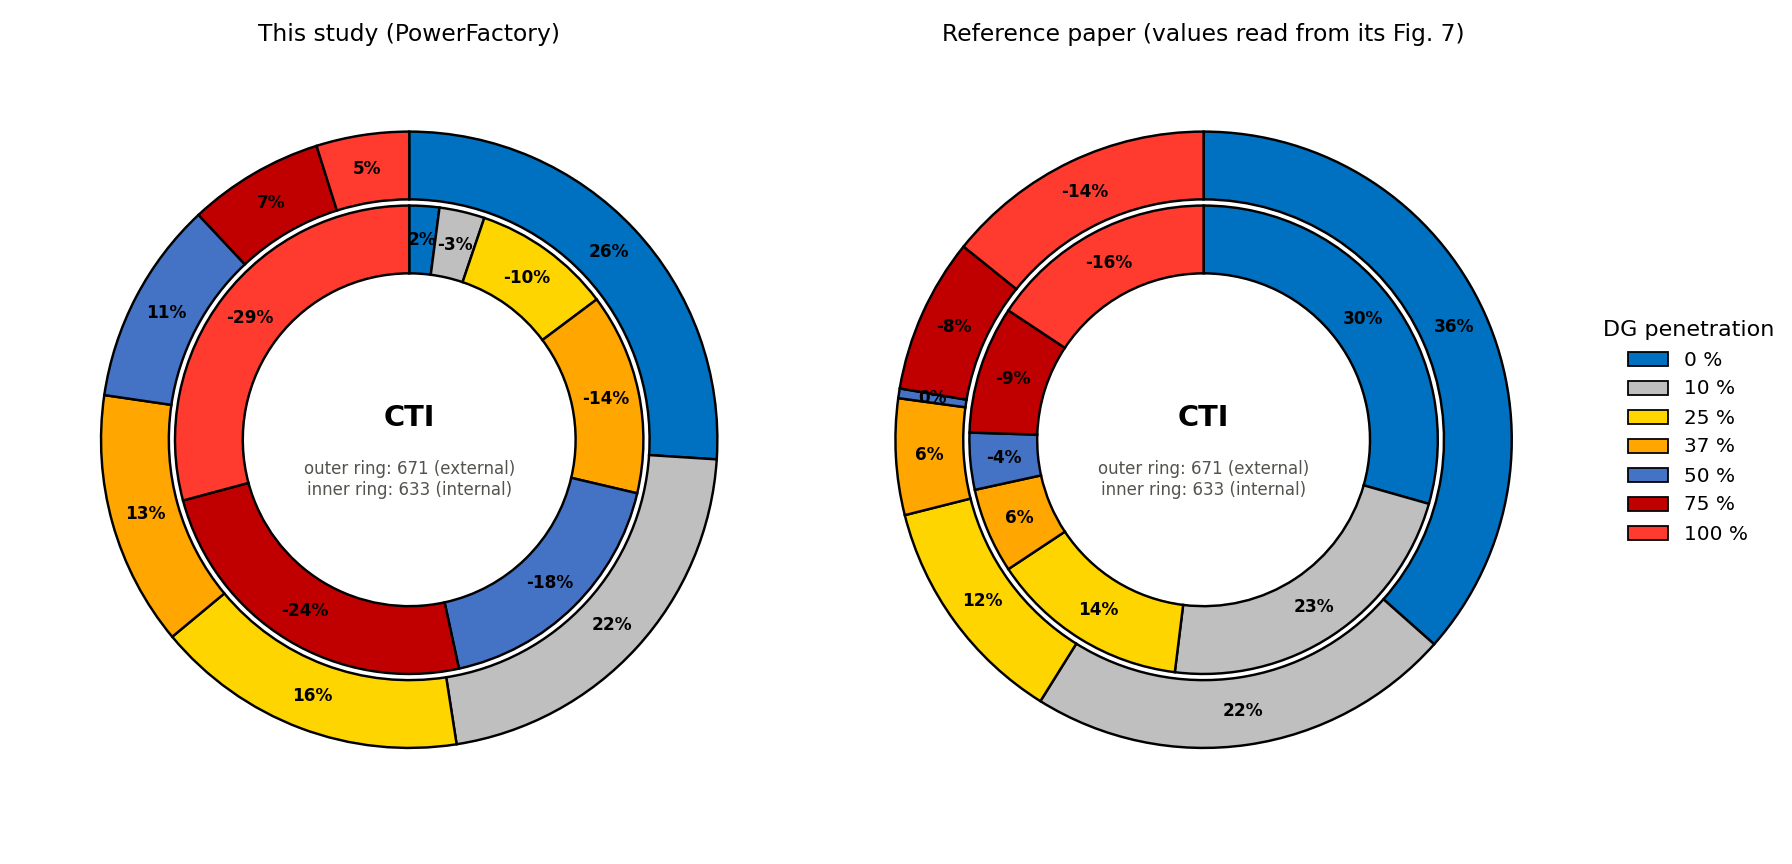
\includegraphics[width=\textwidth]{pen_ring_vs_paper.png}
\caption{CTI against DG penetration: this study (left) and the values read from the paper's Fig.~7 (right).}
\label{fig:e7}
\end{figure}

\begin{table}[H]
\centering\small
\begin{tabular}{|c|c|c|c|c|}
\hline
 & \multicolumn{2}{c|}{\textbf{Node 633 (ring \%)}} & \multicolumn{2}{c|}{\textbf{Node 671 (ring \%)}} \\
\textbf{DG (\%)} & \textbf{this study} & \textbf{paper} & \textbf{this study} & \textbf{paper} \\ \hline
0 & $+2.1$ & $+30$ & $+26.0$ & $+36$ \\ \hline
10 & $-3.1$ & $+23$ & $+21.5$ & $+22$ \\ \hline
25 & $-9.6$ & $+14$ & $+16.4$ & $+12$ \\ \hline
37 & $-13.9$ & $+6$ & $+13.4$ & $+6$ \\ \hline
50 & $-17.9$ & $-4$ & $+10.7$ & $+0$ \\ \hline
75 & $-24.2$ & $-9$ & $+7.1$ & $-8$ \\ \hline
100 & $-29.2$ & $-16$ & $+4.9$ & $-14$ \\ \hline
\end{tabular}
\caption{CTI shares against DG penetration: this study and the paper's Fig.~7.}
\label{tab:e7}
\end{table}

% =====================================================================================================
\appendixhead{C}{PYTHON SCRIPTS}
The model, the studies and the evaluation of the coordination were run in DIgSILENT \PF{} through its Python
interface. This appendix lists the scripts in the order in which they are run. Table~\ref{tab:scripts} gives
the purpose of each script.

\begin{table}[H]
\centering\small
\begin{tabularx}{\textwidth}{|l|L|}
\hline
\textbf{Script} & \textbf{Purpose} \\ \hline
\texttt{show\_progress.py} & Script of the PowerFactory script object Final(1): runs the load flows, the short-circuit database and the coordination study, and prints the report in the Output Window \\ \hline
\texttt{pf\_setup.py} & Connection to PowerFactory and helper functions \\ \hline
\texttt{protection\_data.py} & Feeder, device and fault data \\ \hline
\texttt{curves.py} & Relay and fuse time--current curves \\ \hline
\texttt{step1\_build\_model.py} & Builds the protection devices and the DG in the model \\ \hline
\texttt{step2\_studies.py} & Unbalanced load flow and short-circuit studies \\ \hline
\texttt{step3\_design\_and\_evaluate.py} & Settings, fuse coefficients and classification of the coordination \\ \hline
\texttt{step4\_apply\_settings.py} & Writes the settings into the relay and fuse elements of the model \\ \hline
\texttt{step5\_fig10\_emt.py} & EMT simulation of the reclosing sequence \\ \hline
\end{tabularx}
\caption{Python scripts of the study.}
\label{tab:scripts}
\end{table}

\subsection*{C.1\quad \texttt{show\_progress.py}}
Script of the PowerFactory script object Final(1): runs the load flows, the short-circuit database and the coordination study, and prints the report in the Output Window.
\begin{lstlisting}
"""
Script behind the PowerFactory script object "Final(1)".  The report appears in the Output Window.

First (always)     load flow on all buses and branches, "From node -> To node", DG disconnected
                   and connected                                          loadflow_all_buses.py

Stage 1 (RUN_DATABASE)  load-flow and short-circuit database, DG disconnected and connected, with the
                   current through R1 and R2 and its direction, If,max, If,min and a validation
                   checklist                                                  database_study.py
                   -> results/database/  (no relay or fuse setting is touched)

Stage 2 (only when RUN_COORDINATION = True, i.e. after the database has been checked)
                   design by the paper's method: Tables II, III, IV, Figs. 14, 17;
                   settings written into the model and PowerFactory's trip times checked;
                   Tables I-IV (Table IV with the fuse t_MMT) -> results/database/   make_tables.py
                                                    step2_studies.py, step3_..., step4_...

While it runs, PowerFactory fills the Output Window with its own messages (a fault on a phase a
bus does not have is reported as "Short-circuit calculation not possible"; that is normal).  At the
end the window is cleared and only the report is printed.  The report is also saved as
results/Show_Progress_output.txt.

Replaces the old Show_Progress.py, which needs relays named "R1" and "R2"; in this model they are
"R1 Fast", "R1 Delayed", "R2 Fast", "R2 Delayed", "R2 Rev Fast", "R2 Rev Delayed".

Run: Python Script (ComPython) -> Execute.  The model is left in the study case
"Study with Substation Transformer".
"""

import contextlib
import csv
import gc
import io
import os
import runpy
import subprocess
import sys
import traceback

DIR = r"C:\Users\Rabin\Desktop\Digsilent_project - TWIST AND TURN\DSDR_Study"
if not os.path.isdir(DIR):
    DIR = os.path.dirname(os.path.abspath(__file__))
RES = os.path.join(DIR, "results")
OUT_TXT = os.path.join(RES, "Show_Progress_output.txt")
RUN_DATABASE = True           # False: only the load flow on all buses and branches
RUN_COORDINATION = True       # stage 2 after the database; switched on 2026-10-01 (database accepted)
OWN = ("pf_setup", "protection_data", "curves", "step3_design_and_evaluate")


def forget():
    """PowerFactory keeps its Python session between runs: drop this project's modules (and with
    them the Application object of an earlier run) so every run starts clean."""
    for m in OWN:
        sys.modules.pop(m, None)
    gc.collect()


forget()
if DIR not in sys.path:
    sys.path.insert(0, DIR)
import pf_setup

app = pf_setup.get_app()
report = []
pf_setup.out = lambda msg="": report.append(str(msg))      # the steps' messages go into the report


def banner(text):
    report.extend(["", "#" * 100, "#  " + text, "#" * 100])


def step(script, *args):
    """Run one step of the pipeline; what it prints goes into the report."""
    argv = getattr(sys, "argv", None)
    sys.argv = [script] + list(args)
    buf = io.StringIO()
    try:
        with contextlib.redirect_stdout(buf):
            runpy.run_path(os.path.join(DIR, script), run_name="__main__")
    finally:
        report.extend(buf.getvalue().splitlines())
        if argv is None:
            del sys.argv
        else:
            sys.argv = argv
        sys.modules.pop("step3_design_and_evaluate", None)   # step 4 must read the new results


def external(script):
    """Run a step that needs no PowerFactory with the normal python.exe: PowerFactory's built-in
    interpreter is some 50 times slower on pure calculation (step 3: 13 minutes instead of 15 s)."""
    exe = os.path.join(os.path.dirname(os.path.dirname(os.__file__)), "python.exe")
    if not os.path.isfile(exe):
        return step(script)
    env = dict(os.environ, PYTHONIOENCODING="utf-8")
    p = subprocess.run([exe, os.path.join(DIR, script)], cwd=DIR, env=env, stdout=subprocess.PIPE,
                       stderr=subprocess.STDOUT, creationflags=getattr(subprocess, "CREATE_NO_WINDOW", 0))
    report.extend(p.stdout.decode("utf-8", "replace").splitlines())
    if p.returncode:
        raise RuntimeError("%s failed (exit code %d)" % (script, p.returncode))


def grid(title, column):
    """Fig. 14 / 17 as text: one symbol per faulted node and fault type."""
    rows = list(csv.DictReader(open(os.path.join(RES, "Fig14_Fig17_classification.csv"))))
    nodes = []
    for r in rows:
        if r["node"] not in nodes:
            nodes.append(r["node"])
    sym = {"held": "v", "lost": "x", "n/a": "-"}
    report.extend(["", "   " + title, "   (v) exists   (x) doesn't exist   (-) not applicable"])
    for ft in ("LG", "LL", "LLG", "LLL"):
        cells = {r["node"]: sym[r[column]] for r in rows if r["fault"] == ft}
        report.append("   %-4s |" % ft + "".join("  (%s) " % cells[n] for n in nodes))
    report.append("        +" + "-" * (6 * len(nodes)) + "> faulted node")
    report.append("         " + "".join(" %-5s" % n for n in nodes))


def run():
    app.PrintPlain("Running. PowerFactory's messages below are replaced by the report at the end.")
    app.EchoOff()
    banner("LOAD FLOW ON ALL BUSES AND BRANCHES  (From node -> To node; no setting is changed)")
    step("loadflow_all_buses.py")
    if not RUN_DATABASE:
        report.extend(["", "Short-circuit database and relay coordination not run: RUN_DATABASE = False in show_progress.py."])
        return
    banner("STAGE 1 - LOAD-FLOW AND SHORT-CIRCUIT DATABASE  (no relay or fuse setting is changed)")
    step("database_study.py")
    if not RUN_COORDINATION:
        report.extend(["", "Relay coordination (pickup, fast / delayed operation, TDS, TCC, CTI) has NOT been run:",
                       "RUN_COORDINATION = False in show_progress.py. Set it to True once the database is accepted."])
        return
    banner("STAGE 2 - RELAY COORDINATION")
    banner("1. LOAD FLOWS AND SHORT CIRCUITS  (PowerFactory, complete method, unbalanced)")
    step("step2_studies.py")
    banner("2. DESIGN BY THE PAPER'S METHOD  -  Tables II, III, IV; Figs. 14, 17")
    external("step3_design_and_evaluate.py")
    banner("FIG. 14 AND FIG. 17  -  recloser-fuse coordination, DG 4.05 MVA at 692")
    grid("Fig. 14: without the DSDR", "without DSDR (Fig14)")
    grid("Fig. 17: with the DSDR", "with DSDR (Fig17)")
    banner("3. DSDR SETTINGS IN THE MODEL  -  PowerFactory's trip times against the calculation")
    step("step4_apply_settings.py", "dsdr")
    banner("4. TABLES I-IV OF THE PAPER  (Table IV with the fuse t_MMT and t_TCT)  -> results/database/")
    external("make_tables.py")
    external("make_figures_1_to_6.py")
    report.extend(["", "Figures: " + os.path.join(RES, "figures") + "  (Fig01 ... Fig17)",
                   "Tables:  " + os.path.join(RES, "database") + "  (Table_I ... Table_IV csv, Tables_I_to_IV.txt)"])


try:
    try:
        run()
    except Exception:
        report.extend(["", "SCRIPT STOPPED WITH AN ERROR:"] + ["  " + s for s in traceback.format_exc().splitlines()])
        raise
    finally:
        try:
            app.EchoOn()
            app.GetOutputWindow().Clear()
        except Exception:
            pass
        for line in report:
            app.PrintPlain(line)
        with open(OUT_TXT, "w", encoding="utf-8") as fh:
            fh.write("\n".join(report) + "\n")
        app.PrintPlain("Report saved: " + OUT_TXT)
finally:
    del app
    forget()
\end{lstlisting}

\subsection*{C.2\quad \texttt{pf\_setup.py}}
Connection to PowerFactory and helper functions.
\begin{lstlisting}
"""
Shared PowerFactory helpers for the replication of

  M. Yousaf, A. Jalilian, K. M. Muttaqi, D. Sutanto, "An Adaptive Overcurrent Protection Scheme
  for Dual-Setting Directional Recloser and Fuse Coordination in Unbalanced Distribution Networks
  With Distributed Generation", IEEE Trans. Ind. Appl., 58(2), 1831-1842, 2022.

Runs either inside PowerFactory (ComPython) or from a normal Python 3.9 shell (engine mode).
"""

import os
import sys

PF_DIR = r"C:\Program Files\DIgSILENT\PowerFactory 2021 SP2"
PROJECT = "IEEE13 DSDR Fuse Coordination"
PFD_FILE = os.path.join(os.path.dirname(os.path.dirname(os.path.abspath(__file__))),
                        "IEEE 13 Node Feeder.pfd")
# The IEEE short-circuit benchmark (Kersting & Shirek 2012, used in ref. [8]) includes the
# 115/4.16 kV 5 MVA substation transformer; this study case reproduces it within ~2 %.
STUDY_CASE = "Study with Substation Transformer"
# Protection devices are built in the base network (this case has no active variation), so they
# exist in every study case; the substation transformer case then adds only its variation.
BUILD_CASE = "Study Detailed Network Model"

HERE = os.path.dirname(os.path.abspath(__file__))
RESULTS = os.path.join(HERE, "results")
os.makedirs(RESULTS, exist_ok=True)

_app = None


def get_app():
    global _app
    if _app is not None:
        return _app
    try:
        import powerfactory as pf                  # inside PowerFactory
    except ImportError:
        os.environ["PATH"] = PF_DIR + ";" + os.environ["PATH"]
        sys.path.append(os.path.join(PF_DIR, "Python", "%d.%d" % sys.version_info[:2]))
        import powerfactory as pf
    _app = pf.GetApplication()
    if _app is None:
        raise RuntimeError("Could not start PowerFactory")
    return _app


def attr(obj, name, default=None):
    try:
        v = obj.GetAttribute(name)
        return default if v is None else v
    except Exception:
        return default


def out(msg=""):
    print(msg)
    try:
        get_app().PrintPlain(msg)
    except Exception:
        pass


def activate(build=False):
    """Activate the replication project (importing the .pfd the first time) and the study case
    (BUILD_CASE for model changes, STUDY_CASE for calculations)."""
    app = get_app()
    user = app.GetCurrentUser()
    prj = user.GetContents(PROJECT + ".IntPrj")
    if not prj:
        before = {p.loc_name for p in user.GetContents("*.IntPrj")}
        imp = user.CreateObject("CompfdImport", "import")
        imp.SetAttribute("e:g_file", PFD_FILE)
        imp.SetAttribute("g_target", user)
        imp.Execute()
        imp.Delete()
        new = [p for p in user.GetContents("*.IntPrj") if p.loc_name not in before]
        new[0].SetAttribute("loc_name", PROJECT)
        prj = [new[0]]
    prj[0].Activate()
    clean_variation()
    name = BUILD_CASE if build else STUDY_CASE
    case = app.GetProjectFolder("study").GetContents(name + ".IntCase", 1)[0]
    case.Activate()
    ldf = app.GetFromStudyCase("ComLdf")
    ldf.SetAttribute("iopt_net", 1)                # unbalanced 3-phase load flow
    return app


# The "Substation Transformer" variation as delivered in the .pfd: 13 objects.  Anything else in its
# stage was recorded by a script (or a click) that changed the network while STUDY_CASE was active -
# DG in / out, relay or fuse settings, a breaker closed - and overrides the base network from then on.
_ORIGINAL_STAGE = {"Substation Transformer": {
    "Terminal", "2-Winding Transformer", "Cub_1", "Switch", "Cub_5", "Switch(1)", "External Grid(1)", "Cub_2",
    "Switch(2)", "Cub_4", "External Grid", "GND611(1)", "Cub_6"}}


def clean_variation():
    """Restore the variation stage to its original objects, so that the base network applies."""
    app = get_app()
    n = 0
    for st in app.GetActiveProject().GetContents("*.IntSstage", 1):
        keep = _ORIGINAL_STAGE.get(st.loc_name)
        if keep is None:
            continue
        for o in st.GetContents():
            if o.loc_name not in keep:
                o.Delete()
                n += 1
    return n


def obj(name, cls):
    hits = get_app().GetCalcRelevantObjects("%s.%s" % (name, cls))
    if not hits:
        raise KeyError("%s.%s not found" % (name, cls))
    return hits[0]


def lib_type(pattern, must_contain=""):
    hits = [h for h in get_app().GetGlobalLibrary().GetContents(pattern, 1)
            if must_contain in h.GetFullName() and "\\Arch\\" not in h.GetFullName()
            and "\\v001\\" not in h.GetFullName()]
    if not hits:
        raise KeyError("library type %s (%s) not found" % (pattern, must_contain))
    return hits[0]


def dg_units():
    return get_app().GetCalcRelevantObjects("*.ElmSym")


def save_table1():
    """Read the DG and its transformer back from the model -> results/Table_I_model.json (Table I)."""
    import json
    sym = dg_units()[0]
    typ = sym.typ_id
    tr = obj("2-Winding Transformer", "ElmTr2").typ_id
    keys = ("sgn", "ugn", "iturbo", "xl", "rstr", "xd", "xq", "xds", "xqs", "xdss", "xqss", "tds0", "tdss0", "tqs0",
            "tqss0", "h")
    data = {k: round(float(attr(typ, k, float("nan"))), 5) for k in keys}
    data.update(tr_strn=round(attr(tr, "strn"), 4), tr_hv=round(attr(tr, "utrn_h"), 4), tr_lv=round(attr(tr, "utrn_l"), 4),
                tr_uk=round(attr(tr, "uktr"), 4), node=sym.bus1.cterm.loc_name, type=typ.loc_name)
    with open(os.path.join(RESULTS, "Table_I_model.json"), "w") as fh:
        json.dump(data, fh, indent=1)
    return data


def set_dg(in_service):
    for g in dg_units():
        g.SetAttribute("outserv", 0 if in_service else 1)
\end{lstlisting}

\subsection*{C.3\quad \texttt{protection\_data.py}}
Feeder, device and fault data.
\begin{lstlisting}
"""
Protection data of the IEEE 13-node feeder (Fig. 6 of Yousaf et al. 2022) and the paper's
published values, used by every other script.

Sources for device data the 2022 paper does not print:
  [8]  M. Yousaf, K. M. Muttaqi, D. Sutanto, "Overcurrent protection scheme for the IEEE 13-node
       benchmark test feeder with improved selectivity", IEEE PES GM 2020, Table V
       (Gould-Shawmut A055C fuses, GE IAC recloser, GE/Alstom CDG relay, gL-800 LV fuse).
  Figs. 8, 9, 11, 12, 13, 15, 16 of the 2022 paper: fuse bands digitised and matched to the
       A055C library curves (melting current at 100 s / 1000 s, within 2 %); used for every
       fuse that a figure shows (F632, F633, F646, F671-1, F671-2, F684, F692, F692-R).
"""

# --------------------------------------------------------------------------------------------
# Device locations.  ("line", name, side)  -> cubicle of branch `name` at `side` (bus1/bus2/buslv)
#                    ("load", name)        -> cubicle of load `name`
# --------------------------------------------------------------------------------------------
# Fuse sizes: the size drawn in the 2022 paper's own figures where a figure shows the fuse (bands
# digitised and matched to the A055C library curves), otherwise ref. [8] Table V.  The figure sizes
# take precedence because they are what the 2022 results were produced with: with [8]'s smaller
# F671-2 (200E) the fuse melts in the second fast shot of Fig. 10 (0.62 s) instead of after both
# shots (paper 1.21 s; 300E gives 1.25 s).  The two papers name some devices differently
# ([8] Fig. 1 against Fig. 6 of the 2022 paper):
#   [8] REC1, REC2  = reclosers R1, R2 of the 2022 paper
#   [8] R1, R2, R5  = overcurrent relays at 632 and 671 - not used in the 2022 scheme, neglected
#   [8] F671        = fuse at 671 towards 684            -> F671-2 here
#   [8] F671-R      = fuse of the load L671              -> F671 here
#   F632 (632-645) and F671-1 (671-692) replace [8]'s relays R1 and R5; they are not in [8], so
#   their sizes come from the fuse bands of the 2022 paper's figures.
#   [8] also fuses the capacitors (F-C611 50E, F-C675 125E); Fig. 6 of the 2022 paper has no
#   capacitor fuses, so they are not modelled.
FUSES = {
    #  name      location                              library type   source of the size
    "F632":   (("line", "LOHL632-645", "bus1"),      "A055C400E", "2022 Figs. 12, 15, 16 (not in [8]: relay R1 there)"),
    "F633":   (("line", "LOHL632-633", "bus1"),      "A055C250E", "[8] Table V"),
    "F634":   (("line", "XFM-1", "buslv"),           "gL-800A",   "[8] Table V (IEC 60269 gL 800 A)"),
    "F645":   (("load", "L645-YcPQ"),                "A055C250E", "[8] Table V"),
    "F646":   (("line", "LOHL645-646", "bus1"),      "A055C300E", "2022 Figs. 11, 15, 16 ([8]: 200E)"),
    "F-DL":   (("line", "LDL", "bus1"),              "A055C250E", "[8] Table V"),
    "F671":   (("load", "L571-DcPQ"),                "A055C250E", "[8] Table V (F671-R there)"),
    "F671-1": (("line", "Switch", "bus1"),           "A055C300E", "2022 Fig. 9 (not in [8]: relay R5 there)"),
    "F692":   (("load", "L692-DcI"),                 "A055C200E", "[8] Table V"),
    "F692-R": (("line", "LC692-675", "bus1"),        "A055C250E", "2022 Fig. 9 ([8]: 300E)"),
    "F675":   (("load", "L675-YcPQ"),                "A055C200E", "[8] Table V"),
    "F671-2": (("line", "LOHL671-684", "bus1"),      "A055C300E", "2022 Fig. 8 ([8]: 200E, F671 there)"),
    "F684":   (("line", "LOHL684-611", "bus1"),      "A055C200E", "2022 Fig. 8 ([8]: 150E)"),
    "F611":   (("load", "L611-YcI"),                 "A055C125E", "[8] Table V"),
    "F652":   (("line", "LC684-652A", "bus1"),       "A055C150E", "[8] Table V"),
}

# Reclosers.  R1: feeder recloser (GE IAC77B801A, extremely inverse, TDS 0.5 / 10 - paper).
#             R2: mid-line recloser on 632-671 at the 671 end (GE/Alstom CDG34, extremely inverse).
RECLOSERS = {
    "R1": dict(loc=("line", "LOHL650-632", "bus1"), relay="IAC77B801A", ct=900.0),
    "R2": dict(loc=("line", "LOHL632-671end", "bus2"), relay="CDG34", ct=500.0),
}
R2_UNITS = ["R2 Fast", "R2 Delayed", "R2 Rev Fast", "R2 Rev Delayed"]

# Distributed load: the middle lump is moved behind a short lateral nDL - DL so that a fault at
# "DL" lies below fuse F-DL, as drawn in Fig. 6.
DL_LUMP = "DistributedLoad"

# --------------------------------------------------------------------------------------------
# Fault locations of Figs. 14 / 17 and Table IV.  Nodes upstream of R2 are in R1's zone.
# phases: conductors present at the node.  primary: fuse feeding the node (Table IV "Fuse").
# path: fuses in series from the fault towards the source (primary first).
# --------------------------------------------------------------------------------------------
NODES = {
    "632": dict(phases="ABC", zone="R1", path=[]),
    "633": dict(phases="ABC", zone="R1", path=["F633"]),
    "634": dict(phases="ABC", zone="R1", path=["F634", "F633"], lv=True),
    "645": dict(phases="BC",  zone="R1", path=["F632"]),
    "646": dict(phases="BC",  zone="R1", path=["F646", "F632"]),
    "DL":  dict(phases="ABC", zone="R1", path=["F-DL"]),
    "671": dict(phases="ABC", zone="R2", path=[]),
    "692": dict(phases="ABC", zone="R2", path=["F671-1"]),
    "675": dict(phases="ABC", zone="R2", path=["F692-R", "F671-1"]),
    "680": dict(phases="ABC", zone="R2", path=[]),
    "684": dict(phases="AC",  zone="R2", path=["F671-2"]),
    "652": dict(phases="A",   zone="R2", path=["F652", "F671-2"]),
    "611": dict(phases="C",   zone="R2", path=["F684", "F671-2"]),
}
NODE_ORDER = ["632", "633", "634", "645", "646", "671", "692", "675", "680", "684", "652", "611", "DL"]
FAULT_TYPES = ["LG", "LL", "LLG", "LLL"]
PF_FAULT = {"LG": "spgf", "LL": "2psc", "LLG": "2pgf", "LLL": "3rst"}

# Branches of Table II:  label -> (branch, side of the measuring cubicle, downstream nodes)
TABLE2_BRANCHES = [
    ("RG60", "632",      "LOHL650-632", "bus1", ["632", "633", "645", "646", "DL", "671", "692", "675", "680", "684", "652", "611"]),
    ("632", "633",       "LOHL632-633", "bus1", ["633"]),
    ("632", "645",       "LOHL632-645", "bus1", ["645", "646"]),
    ("632", "671",       "LOHL632-671end", "bus2", ["671", "692", "675", "680", "684", "652", "611"]),
    ("XFM1-HV", "side",  "XFM-1", "bushv", ["634"]),
    ("XFM1-LV", "side",  "XFM-1", "buslv", ["634"]),
    ("645", "646",       "LOHL645-646", "bus1", ["646"]),
    ("671", "692",       "Switch", "bus1", ["692", "675"]),
    ("671", "684",       "LOHL671-684", "bus1", ["684", "652", "611"]),
    ("671", "680",       "LOHL671-680", "bus1", ["680"]),
    ("692", "675",       "LC692-675", "bus1", ["675"]),
    ("684", "611",       "LOHL684-611", "bus1", ["611"]),
    ("684", "652",       "LC684-652A", "bus1", ["652"]),
]

# --------------------------------------------------------------------------------------------
# Published values (for comparison only)
# --------------------------------------------------------------------------------------------
PAPER_TABLE2 = {  # (from, to): (Inom A, If,min kA, If,max kA)
    ("RG60", "632"): (587.1, 1.24, 5.41), ("632", "633"): (81.1, 0.72, 6.73),
    ("632", "645"): (143.3, 0.93, 4.25), ("632", "671"): (478.2, 1.08, 4.52),
    ("XFM1-HV", "side"): (81.1, 0.73, 6.48), ("XFM1-LV", "side"): (704.7, 0.59, 18.76),
    ("645", "646"): (64.9, 0.84, 3.64), ("671", "692"): (229.3, 0.78, 3.69),
    ("671", "684"): (70.9, 0.69, 3.47), ("671", "680"): (0.0, 0.59, 6.25),
    ("692", "675"): (205.9, 0.71, 7.83), ("684", "611"): (70.8, 0.63, 1.93),
    ("684", "652"): (63.1, 0.66, 2.67),
}
PAPER_TABLE3 = {"F632": 6.38, "F633": 6.83, "F634": 8.32, "F645": 6.65, "F646": 6.67, "F-DL": 6.54,
                "F611": 6.19, "F692": 6.13, "F671": 6.08, "F671-1": 5.85, "F671-2": 5.87,
                "F652": 6.17, "F684": 6.15, "F675": 6.19, "F692-R": 6.14}
PAPER_TABLE4 = {  # node: (R1 fast, R1 delayed, R2 fast, R2 delayed, fuse MMT)
    "632": (0.070, 1.398, 0.045, 0.514, None), "633": (0.094, 1.880, 0.052, 0.706, 0.163),
    "645": (0.105, 2.095, 0.087, 1.659, 0.276), "646": (0.128, 2.555, 0.103, 2.046, 0.181),
    "DL": (0.087, 1.733, 0.076, 1.402, 0.248), "671": (0.105, 2.091, 0.068, 1.113, None),
    "692": (0.115, 2.307, 0.072, 1.258, 0.175), "675": (0.121, 2.414, 0.074, 1.332, 0.185),
    "684": (0.125, 2.507, 0.075, 1.394, 0.205), "680": (0.137, 2.747, 0.079, 1.555, None),
    "611": (0.326, 6.523, 0.146, 4.385, 0.417), "652": (0.676, 13.525, 0.143, 9.370, 0.233),
}
# Fig. 14 (without DSDR): cells marked "doesn't exist"; Fig. 17 (with DSDR): none.
PAPER_FIG14_LOST = {("633", "LLG"), ("633", "LLL"), ("645", "LG"), ("645", "LL"), ("645", "LLG"),
                    ("646", "LL"), ("646", "LLG"), ("675", "LLG"), ("675", "LLL")}

OLF = 1.25            # overload factor, eqs. (3) and (12)
A_FUSE = -1.8         # fuse slope a_i, eq. (6)
T_RECL_MIN = 10 / 60  # minimum time delay between the reclosers' delayed curves (10 cycles)
\end{lstlisting}

\subsection*{C.4\quad \texttt{curves.py}}
Relay and fuse time--current curves.
\begin{lstlisting}
"""
Operating-time curves, identical to the PowerFactory library types (data from studies.json):

  R1  GE IAC77B801A   IAC extremely inverse GES7005B (formula), curve from 1.5 x Ip to 40 x Ip
  R2  GE/Alstom CDG34 CDG14 extremely inverse 398.S23.37 (table of t vs M for TMS 0.1-1.0),
                      curve from 2 x Is to 40 x Is, t >= 0.031 s at any TMS
  fuses               minimum melting (MMT) and total clearing (TCT) tables of the library type
Times are in s, currents in primary A.  A current below a curve's start returns inf (no trip).
"""

import math

INF = float("inf")


def _loglog(x, pts):
    """Log-log interpolation in a sorted list of (x, y); None outside the range."""
    if x < pts[0][0] or x > pts[-1][0]:
        return None
    for (x1, y1), (x2, y2) in zip(pts, pts[1:]):
        if x1 <= x <= x2:
            if x2 == x1:
                return y1
            f = (math.log(x) - math.log(x1)) / (math.log(x2) - math.log(x1))
            return math.exp(math.log(y1) + f * (math.log(y2) - math.log(y1)))
    return pts[-1][1]


class IAC:
    """IAC extremely inverse: t = TDS (0.004 + 0.6379/(M-0.62) + 1.7872/(M-0.62)^2 + 0.2461/(M-0.62)^3)."""

    def __init__(self, data):
        self.imin, self.imax = data["imin"], data["imax"]

    def t(self, i, ip, tds):
        m = i / ip
        if m < self.imin:
            return INF
        x = min(m, self.imax) - 0.62
        return tds * (0.004 + 0.6379 / x + 1.7872 / x ** 2 + 0.2461 / x ** 3)


class CDG:
    """CDG14 extremely-inverse table, log-log in M, linear in TMS (extrapolated below 0.1)."""

    def __init__(self, data):
        rows = data["vmat"]
        self.tms = rows[0][1:]
        self.rows = rows[1:]
        self.imin, self.imax, self.tmin = data["imin"], data["imax"], data["tmin"]

    def t(self, i, ip, tms):
        m = i / ip
        if m < self.imin:
            return INF
        m = min(m, self.imax)
        col = [_loglog(m, [(r[0], r[j + 1]) for r in self.rows]) for j in range(len(self.tms))]
        k = max(0, min(len(self.tms) - 2, next((j for j in range(len(self.tms) - 1)
                                                if tms <= self.tms[j + 1]), len(self.tms) - 2)))
        f = (tms - self.tms[k]) / (self.tms[k + 1] - self.tms[k])
        return max(self.tmin, col[k] + f * (col[k + 1] - col[k]))    # tmin is absolute (as in PF)


class Fuse:
    def __init__(self, data):
        m = data["vmat"]
        self.irat = data["irat"]
        self.melt = sorted((r[0], r[1]) for r in m if r[0] > 0)
        self.clear = sorted((r[2], r[3]) for r in m if r[2] > 0)

    @staticmethod
    def _t(pts, i):
        if i < pts[0][0]:
            return INF
        if i > pts[-1][0]:
            return pts[-1][1]
        return _loglog(i, pts)

    def mmt(self, i):
        return self._t(self.melt, i)

    def tct(self, i):
        return self._t(self.clear, i)

    def i_at_mmt(self, t):
        """Current that melts the fuse in t seconds."""
        pts = sorted((b, a) for a, b in self.melt)
        return _loglog(t, pts)
\end{lstlisting}

\subsection*{C.5\quad \texttt{step1\_build\_model.py}}
Builds the protection devices and the DG in the model.
\begin{lstlisting}
"""
Step 1 - build the protection system of Fig. 6 in a clean copy of the IEEE 13-node feeder.

  * removes every relay, fuse and CT left in the project (fresh start)
  * adds the lateral nDL - DL for the distributed-load fuse F-DL (fault location "DL")
  * sets the synchronous DG to the data of Table I
  * places the 15 fuses (Gould-Shawmut A055C / gL, see protection_data.FUSES)
  * places R1 (2 x GE IAC77B801A: fast, delayed) and R2 (4 x GE/Alstom CDG34: forward fast,
    forward delayed, reverse fast, reverse delayed) with their CTs.
Settings are written afterwards by step4_apply_settings.py from results/settings.json.
"""

from pf_setup import activate, attr, out, obj, lib_type, save_table1
from protection_data import FUSES, RECLOSERS, R2_UNITS, DL_LUMP

app = activate(build=True)
grid = obj("632", "ElmTerm").GetParent()


def cubicle(loc):
    if loc[0] == "load":
        return obj(loc[1], "ElmLod").GetAttribute("bus1")
    for cls in ("ElmLne", "ElmTr2", "ElmCoup"):
        hits = app.GetCalcRelevantObjects("%s.%s" % (loc[1], cls))
        if hits:
            return hits[0].GetAttribute(loc[2])
    raise KeyError(loc)


# ---- 1. fresh start --------------------------------------------------------------------------
n = 0
for cls in ("ElmRelay", "RelFuse", "StaCt"):
    for o in grid.GetContents("*." + cls, 1):
        o.Delete()
        n += 1
for f in app.GetProjectFolder("equip").GetContents("Fuse Types Yousaf 2022*"):
    f.Delete()
out("Removed %d old protection objects" % n)

# ---- 2. distributed-load lateral nDL - DL ------------------------------------------------------
if not app.GetCalcRelevantObjects("DL.ElmTerm"):
    ndl = obj("nDL", "ElmTerm")
    dl = grid.AddCopy(ndl, "DL")
    for c in dl.GetContents("*.StaCubic"):
        c.Delete()
    proto = obj("LOHL632-671start", "ElmLne")
    line = grid.AddCopy(proto, "LDL")
    line.SetAttribute("bus1", ndl.CreateObject("StaCubic", "Cub_LDL"))
    line.SetAttribute("bus2", dl.CreateObject("StaCubic", "Cub_LDL"))
    line.SetAttribute("dline", 10.0)                  # 10 ft (project length unit)
    load = obj(DL_LUMP, "ElmLod")
    old = load.GetAttribute("bus1")
    load.SetAttribute("bus1", dl.CreateObject("StaCubic", "Cub_Load"))
    old.Delete()
    out("Added terminal DL and 10 ft lateral LDL (config 601); %s moved to DL" % DL_LUMP)

# ---- 3. DG of Table I --------------------------------------------------------------------------
sym = obj("Synchronous Machine", "ElmSym")
typ = sym.typ_id
table1 = dict(xl=0.05, rstr=0.0014, xd=1.4, xq=1.372, xds=0.231, xqs=0.8, xdss=0.118, xqss=0.118,
              tds0=5.5, tdss0=0.05, tqs0=1.25, tqss0=0.19, h=0.75)
# The machine type takes short-circuit time constants; convert Table I's open-circuit ones.
sc_tc = dict(tds=5.5 * 0.231 / 1.4, tdss=0.05 * 0.118 / 0.231, tqs=1.25 * 0.8 / 1.372,
             tqss=0.19 * 0.118 / 0.8)
# Table I gives X'q and T'q0, i.e. a round-rotor machine; with the salient-pole model PowerFactory
# ignores them and reads T''q as T''q0 * X''q / Xq, which turns T''q0 = 0.19 s into 0.326 s.
for k, v in [("iturbo", 1)] + list(table1.items()) + list(sc_tc.items()):
    try:
        typ.SetAttribute(k, v)
    except Exception:
        pass
out("DG (%s): %s" % (typ.loc_name, ", ".join("%s=%s" % (k, round(attr(typ, k, float("nan")), 4))
                                              for k in table1)))
save_table1()

# ---- 4. fuses ---------------------------------------------------------------------------------
for name, (loc, tname, src) in FUSES.items():
    cub = cubicle(loc)
    f = cub.CreateObject("RelFuse", name)
    f.typ_id = lib_type(tname + ".TypFuse", "ProtFuse")
    out("  %-7s %-10s at %-6s (%s)" % (name, tname, cub.GetAttribute("cterm").loc_name, src))


# ---- 5. reclosers -----------------------------------------------------------------------------
def ct_type(prim):
    equip = app.GetProjectFolder("equip")
    name = "CT %.0f-5A" % prim
    hit = equip.GetContents(name + ".TypCt")
    t = hit[0] if hit else equip.CreateObject("TypCt", name)
    t.SetAttribute("primtaps", [prim])
    t.SetAttribute("sectaps", [5.0])
    return t


def add_relay(cub, name, rtype):
    r = cub.CreateObject("ElmRelay", name)
    r.typ_id = rtype
    r.SlotUpdate()
    for e in r.GetContents("*.RelIoc") + r.GetContents("*Earth*.RelToc"):
        e.SetAttribute("outserv", 1)                   # phase time-overcurrent only
    return r


iac = lib_type("IAC77B801A.TypRelay", "ProtRelay\\GE\\IAC\\60Hz")
cdg = lib_type("CDG34-5A (1-4).TypRelay", "CDG34 A & B & C\\Prefered Taps")
for rname, cfg in RECLOSERS.items():
    cub = cubicle(cfg["loc"])
    ct = cub.CreateObject("StaCt", "CT " + rname)
    ct.typ_id = ct_type(cfg["ct"])
    ct.SetAttribute("ptapset", cfg["ct"])
    ct.SetAttribute("stapset", 5.0)
    units = ["R1 Fast", "R1 Delayed"] if rname == "R1" else R2_UNITS
    for u in units:
        add_relay(cub, u, iac if rname == "R1" else cdg)
    out("  %s: %s at %s, CT %.0f/5, units %s" % (rname, cfg["relay"], cub.GetAttribute("cterm").loc_name,
                                                cfg["ct"], ", ".join(units)))

ldf = app.GetFromStudyCase("ComLdf")
out("Load flow after build: %s" % ("OK" if ldf.Execute() == 0 else "FAILED"))
\end{lstlisting}

\subsection*{C.6\quad \texttt{step2\_studies.py}}
Unbalanced load flow and short-circuit studies.
\begin{lstlisting}
"""
Step 2 - load flows and short circuits in PowerFactory (complete method, unbalanced).

Saves results/studies.json with, for every case, the phase currents (A) through R1, R2, every
fuse and every Table II branch.  The currents do not depend on the protection settings, so the
design (step 3) can be iterated in Python without re-running PowerFactory.

Cases
  loadflow   DG out / DG in                              -> Inom (Table II), reverse current at R2
  max        all nodes x LG/LL/LLG/LLL x phases, Rf = 0, DG out and DG in (100 %)
  min        LG through 3 ohm at all nodes, DG out        -> If,min (Table II)
  pen        LLL at 633 and 671, DG penetration 0-100 %   (kept in studies.json; Fig. 7 is not produced)
  figures    the faults of Figs. 8-13, 15, 16 and Fig. 10 (DG in)
"""

import json
import os

from pf_setup import activate, attr, out, obj, lib_type, RESULTS, dg_units, clean_variation, save_table1
from protection_data import FUSES, RECLOSERS, NODES, NODE_ORDER, PF_FAULT, TABLE2_BRANCHES

app = activate()
ldf = app.GetFromStudyCase("ComLdf")
shc = app.GetFromStudyCase("ComShc")
shc.SetAttribute("iopt_mde", 3)          # complete method (prefault load flow)
shc.SetAttribute("iopt_allbus", 0)

# ---- measuring points ------------------------------------------------------------------------
POINTS = {}
for name, cfg in RECLOSERS.items():
    POINTS[name] = cfg["loc"]
for name, (loc, _, _) in FUSES.items():
    POINTS[name] = loc
for frm, to, br, side, _ in TABLE2_BRANCHES:
    POINTS["%s-%s" % (frm, to)] = ("line", br, side)


def element(loc):
    if loc[0] == "load":
        return obj(loc[1], "ElmLod"), "bus1"
    for cls in ("ElmLne", "ElmTr2", "ElmCoup"):
        hits = app.GetCalcRelevantObjects("%s.%s" % (loc[1], cls))
        if hits:
            return hits[0], loc[2]
    raise KeyError(loc)


ELEMENTS = {k: element(v) for k, v in POINTS.items()}
TERMS = {t.loc_name: t for t in app.GetCalcRelevantObjects("*.ElmTerm")}


def currents(var, scale=1000.0):
    """Phase currents in A (short-circuit results are in kA, load-flow results in A)."""
    res = {}
    for k, (e, side) in ELEMENTS.items():
        res[k] = [round(scale * abs(attr(e, "%s:%s:%s" % (var, side, p), 0.0)), 2) for p in "ABC"]
    return res


# ---- DG penetration ---------------------------------------------------------------------------
sym = dg_units()[0]
dg_tr = obj("2-Winding Transformer", "ElmTr2")
BASE = dict(sgn=attr(sym.typ_id, "sgn"), strn=attr(dg_tr.typ_id, "strn"),
            pgini=attr(sym, "pgini"), qgini=attr(sym, "qgini"))
save_table1()                            # Table I as it is in the model (results/Table_I_model.json)


def set_penetration(p):
    """p = DG rating / 4.05 MVA (4.05 MVA = total feeder load, so 1.0 = 100 %)."""
    if p <= 0:
        sym.SetAttribute("outserv", 1)
        return
    sym.SetAttribute("outserv", 0)
    sym.typ_id.SetAttribute("sgn", BASE["sgn"] * p)
    dg_tr.typ_id.SetAttribute("strn", BASE["strn"] * p)
    sym.SetAttribute("pgini", BASE["pgini"] * p)
    sym.SetAttribute("qgini", BASE["qgini"] * p)


# ---- short circuits ---------------------------------------------------------------------------
PH_ATTR = {"spgf": "i_pspgf", "2psc": "i_p2psc", "2pgf": "i_p2pgf"}


def run_fault(where, ftype, index=0, rf=0.0, xf=0.0, dist=None):
    """where: terminal name, or line name with dist = % from bus1. Returns dict or None."""
    code = PF_FAULT[ftype]
    if dist is None:
        shc.SetAttribute("shcobj", TERMS[where])
    else:
        shc.SetAttribute("shcobj", obj(where, "ElmLne"))
        shc.SetAttribute("ppro", float(dist))
    shc.SetAttribute("iopt_shc", code)
    if code in PH_ATTR:
        shc.SetAttribute(PH_ATTR[code], index)
    shc.SetAttribute("Rf", rf)
    shc.SetAttribute("Xf", xf)
    if shc.Execute() != 0:
        return None
    if dist is None:
        t = TERMS[where]
        ifault = [round(1000.0 * abs(attr(t, "m:Ikss:" + p, 0.0)), 2) for p in "ABC"]
    else:
        ifault = None
    faulted = None
    if ifault:
        big = max(ifault)
        faulted = "".join(p for p, i in zip("ABC", ifault) if big > 0 and i > 0.2 * big)
    return dict(where=where, type=ftype, index=index, rf=rf, dist=dist, phases=faulted,
                ifault=ifault, I=currents("m:Ikss"))


def sweep(dg, rf=0.0, types=("LG", "LL", "LLG", "LLL"), nodes=NODE_ORDER, tag="max"):
    res = []
    for node in nodes:
        for ft in types:
            seen = set()
            for idx in ([0] if ft == "LLL" else [0, 1, 2]):
                r = run_fault(node, ft, idx, rf)
                if r is None or not r["phases"]:
                    continue
                key = r["phases"]
                if ft != "LLL" and (key in seen or len(key) != (1 if ft == "LG" else 2)):
                    continue
                if not set(key) <= set(NODES[node]["phases"]):
                    continue
                seen.add(key)
                r.update(case=tag, dg=dg)
                res.append(r)
    return res


def loadflow(dg_on):
    set_penetration(1.0 if dg_on else 0.0)
    if ldf.Execute() != 0:
        raise RuntimeError("load flow failed")
    res = currents("m:I", 1.0)
    e, side = ELEMENTS["R2"]
    res["R2_P_kW"] = round(attr(e, "m:Psum:%s" % side, 0.0), 1)
    res["DG_P_MW"] = round(attr(sym, "m:Psum:bus1", 0.0) / 1000.0, 3) if dg_on else 0.0
    return res


data = dict(points={k: list(v) for k, v in POINTS.items()})
data["loadflow"] = {"dg_out": loadflow(False), "dg_in": loadflow(True)}
out("Load flow: R2 %.0f kW (DG out) / %.0f kW (DG in)" % (
    data["loadflow"]["dg_out"]["R2_P_kW"], data["loadflow"]["dg_in"]["R2_P_kW"]))

faults = []
set_penetration(0.0)
faults += sweep(0.0, tag="max")
faults += sweep(0.0, rf=3.0, types=("LG",), tag="min")
set_penetration(1.0)
faults += sweep(1.0, tag="max")
faults += sweep(1.0, rf=3.0, types=("LG",), tag="min")
out("Node sweeps: %d faults" % len(faults))

for p in (0.0, 0.10, 0.25, 0.37, 0.50, 0.75, 1.0):
    set_penetration(p)
    for r in sweep(p, types=("LLL",), nodes=["633", "671"], tag="pen"):
        faults.append(r)

# Figure faults (DG in service).  Fig. 9: LLG at the middle of 692-675 through 1 ohm;
# Fig. 13: 3-phase at 10 % of 632-633; Fig. 10: LL (a-c) at 684 through 0.2 ohm.
set_penetration(1.0)
FIG = [("Fig8", "611", "LG", None, 0.0, None), ("Fig9", "LC692-675", "LLG", None, 1.0, 50.0),
       ("Fig10", "684", "LL", "AC", 0.2, None), ("Fig11", "646", "LL", "BC", 1.0, None),
       ("Fig12", "645", "LL", "BC", 1.5, None), ("Fig13", "LOHL632-633", "LLL", None, 0.0, 10.0),
       ("Fig15", "646", "LL", "BC", 0.0, None)]
for fig, where, ft, want, rf, dist in FIG:
    for idx in ([0] if ft in ("LLL",) else [0, 1, 2]):
        r = run_fault(where, ft, idx, rf, dist=dist)
        if r is None:
            continue
        if want and r["phases"] != want:
            continue
        if dist is not None and ft == "LLG" and idx != 1:      # b-c on the 3-phase cable
            continue
        r.update(case=fig, dg=1.0)
        faults.append(r)
        out("  %s: %s %s at %s%s, Rf %.1f -> R1 %.0f A, R2 %.0f A" % (
            fig, ft, r["phases"] or "", where, "" if dist is None else " (%.0f %%)" % dist, rf,
            max(r["I"]["R1"]), max(r["I"]["R2"])))
        break

data["faults"] = faults

# ---- curve data used by the Python analysis (identical to the PowerFactory types) -------------
curves = {"fuses": {}}
for name, (loc, tname, _) in FUSES.items():
    t = obj(name, "RelFuse").typ_id         # keyed by the installed type: step 4 may have revised the size
    curves["fuses"][t.loc_name] = dict(irat=attr(t, "irat"), vmat=[list(r) for r in t.GetAttribute("vmat")])
a055c = lib_type("A055C200E.TypFuse", "ProtFuse").GetParent()
for t in a055c.GetContents("A055C*.TypFuse"):                 # every size, for fuse revision
    curves["fuses"].setdefault(t.loc_name, dict(irat=attr(t, "irat"),
                                                vmat=[list(r) for r in t.GetAttribute("vmat")]))
cdg = obj("R2 Fast", "ElmRelay").GetContents("*.RelToc")[0]
ch = attr(cdg, "pcharac")
curves["cdg"] = dict(name=ch.loc_name, imin=attr(ch, "imin"), imax=attr(ch, "imax"),
                     tmin=attr(ch, "tmin"), vmat=[list(r) for r in ch.GetAttribute("vmat")])
iac = attr(obj("R1 Fast", "ElmRelay").GetContents("Toc.RelToc")[0], "pcharac")
curves["iac"] = dict(name=iac.loc_name, expr=attr(iac, "expr"), imin=attr(iac, "imin"),
                     imax=attr(iac, "imax"))
data["curves"] = curves
set_penetration(1.0)
ldf.Execute()
with open(os.path.join(RESULTS, "studies.json"), "w") as f:
    json.dump(data, f, indent=1)
clean_variation()                       # DG switching above was recorded in the study case's variation
out("Saved %d fault cases to results/studies.json" % len(faults))
\end{lstlisting}

\subsection*{C.7\quad \texttt{step3\_design\_and\_evaluate.py}}
Settings, fuse coefficients and classification of the coordination.
\begin{lstlisting}
"""
Step 3 - protection design by the paper's method (Section II, Fig. 5) and coordination analysis.
Pure Python on results/studies.json (no PowerFactory needed).

The paper's workflow, in three stages:

 A  Design without DG (conventional fuse-saving scheme)
      step 1  load flow -> Inom (Table II)
      step 3  pickups by eq. (3), Ip = OLF x Inom, realised with the relay's CT and taps
              R1  IAC77B801A, TDS 0.5 (fast) / 10 (delayed) - paper
              R2  CDG34 (CDG14 table, curve from 2 x plug).  Fast plug = Ip/2 (curve starts at Ip,
                  as in Figs. 8 and 13), delayed plug = Ip.  Fast TMS = lowest dial 0.1; delayed
                  TMS = highest dial that stays 10 cycles below R1's delayed curve.
      step 4  fuse coefficients b_i, eqs. (6)-(9) -> Table III (i = 1 closest to the fault, [25])
      step 5  fault study; steps 8-10 until every fault is coordinated without DG
 B  DG added (4.05 MVA at 692), settings unchanged -> Fig. 14, Figs. 8-13
 C  R2 as DSDR: reverse pickup eq. (12), TMS revised by If,Rec / If,Fuse (step 8);
    fuse revision (step 9) where a dial limit is reached -> Fig. 17, Table IV, Figs. 15-16

Coordination of one fault ("held"):
  * every recloser that interrupts a source feeding the fault (R1 for the grid in R1's zone,
    R2 for the grid in R2's zone, R2 in reverse for the DG in R1's zone) picks up, trips on its
    fast curve before the primary fuse melts (MMT), and on its delayed curve after the fuse clears
    (TCT);
  * series fuses: TCT(primary) < 0.75 MMT(backup), eq. (8);
  * R2-zone faults: R2 fast before R1 fast and R2 delayed >= 10 cycles before R1 delayed.
A cell of Figs. 14 / 17 is held only if every phase combination of that fault type holds.
"""

import copy
import csv
import json
import math
import os

import matplotlib
matplotlib.use("Agg")
import matplotlib.pyplot as plt
from matplotlib.lines import Line2D

from curves import IAC, CDG, Fuse, INF, _loglog
from protection_data import (FUSES, NODES, NODE_ORDER, FAULT_TYPES, TABLE2_BRANCHES, PAPER_TABLE2,
                             PAPER_TABLE3, PAPER_TABLE4, PAPER_FIG14_LOST, OLF, A_FUSE, T_RECL_MIN)

HERE = os.path.dirname(os.path.abspath(__file__))
RES = os.path.join(HERE, "results")
FIG = os.path.join(RES, "figures")
os.makedirs(FIG, exist_ok=True)

D = json.load(open(os.path.join(RES, "studies.json")))
IACC, CDGC = IAC(D["curves"]["iac"]), CDG(D["curves"]["cdg"])
FTYPE = {t: Fuse(v) for t, v in D["curves"]["fuses"].items()}
A055C = sorted([t for t in FTYPE if t.startswith("A055C")], key=lambda t: FTYPE[t].irat)
FAULTS = D["faults"]
LF = D["loadflow"]
REPORT = []

CDG_TAPS = [1.0, 1.2, 1.5, 2.0, 2.4, 3.0, 4.0]                     # CDG34-5A (1-4), secondary A
IAC_TAPS = [0.5, 0.6, 0.7, 0.8, 1.0, 1.2, 1.5, 2.0, 2.5, 3.0, 4.0]   # IAC77B801A, secondary A
CT_R1, CT_R2, CT_R2RV = 900.0, 1000.0, 500.0
TMS_MIN, TMS_MAX = 0.1, 1.0            # CDG34 dial range
# The DSDR keeps the CDG34 extremely-inverse curve (paper, Section IV-A).  That curve is a table
# for TMS 0.1-1.0 whose times are not proportional to TMS, so the dial is not extended below 0.1
# (PowerFactory's linear extrapolation below 0.1 even gives negative times at low multiples).
DSDR_TMS_MIN = TMS_MIN


def say(s=""):
    print(s)
    REPORT.append(s)


def imax(rec, point):
    return max(rec["I"][point])


def fmt(t, nd=3):
    return "no trip" if t == INF else ("%.*f" % (nd, t))


def save_png(fig, fname):
    """Save a figure; if the file is open in a viewer (locked on Windows) write <name>_new.png."""
    path = os.path.join(FIG, fname)
    alt = path[:-4] + "_new.png"
    try:
        fig.savefig(path, dpi=160)
        if os.path.isfile(alt):
            os.remove(alt)
    except OSError:
        fig.savefig(alt, dpi=160)
        print("NOTE: %s is open in another program; the new figure is %s" % (fname, os.path.basename(alt)))


CMP = os.path.join(RES, "comparison")             # values of the reference paper, for the comparison only
os.makedirs(CMP, exist_ok=True)


def write_csv(name, header, rows):
    path = os.path.join(RES, name)
    try:
        f = open(path, "w", newline="")
    except PermissionError:                      # open in Excel: the old file stays, the new one goes beside it
        f = open(path[:-4] + "_new.csv", "w", newline="")
        print("NOTE: %s is open in another program; the new table is %s_new.csv" % (name, name[:-4]))
    with f:
        w = csv.writer(f)
        w.writerow(header)
        w.writerows(rows)


def faults(case="max", dg=None, node=None, ftype=None, zone=None):
    return [r for r in FAULTS if r["case"] == case and (dg is None or r["dg"] == dg)
            and (node is None or r["where"] == node) and (ftype is None or r["type"] == ftype)
            and (zone is None or (r["where"] in NODES and NODES[r["where"]]["zone"] == zone
                                  and not NODES[r["where"]].get("lv")))]


# =============================================================================================
# Operating times
# =============================================================================================
def t_r1(i, s, mode):
    return IACC.t(i, s["R1"]["ip"], s["R1"]["tds_" + mode])


def t_r2(i, s, unit, mode):
    u = s[unit]
    return CDGC.t(i, u["is_" + mode], u["tms_" + mode])


def fuse(s, name):
    return FTYPE[s["fuses"][name]]


# =============================================================================================
# Coordination of one fault
# =============================================================================================
def evaluate(r, s, dsdr):
    node = r["where"]
    info = NODES[node]
    i1, i2 = imax(r, "R1"), imax(r, "R2")
    reasons, reclosers = [], []                       # reclosers: (name, unit, I, t_fast, t_delayed)
    if info["zone"] == "R2":
        reclosers.append(("R2", "R2fw", i2, t_r2(i2, s, "R2fw", "f"), t_r2(i2, s, "R2fw", "d")))
        t1f, t1d = t_r1(i1, s, "f"), t_r1(i1, s, "d")
        if reclosers[0][3] < INF and not reclosers[0][3] < t1f:
            reasons.append("R2 fast (%.3f s) not before R1 fast (%s s)" % (reclosers[0][3], fmt(t1f)))
        if reclosers[0][4] < INF and t1d < INF and not t1d - reclosers[0][4] >= T_RECL_MIN:
            reasons.append("R2/R1 delayed margin %.3f s < 10 cycles" % (t1d - reclosers[0][4]))
    else:
        reclosers.append(("R1", "R1", i1, t_r1(i1, s, "f"), t_r1(i1, s, "d")))
        if r["dg"] > 0 and i2 >= s["dg_infeed"]:        # DG infeed above the eq. (12) pickup
            unit = "R2rv" if dsdr else "R2fw"
            reclosers.append(("R2 rev" if dsdr else "R2", unit, i2, t_r2(i2, s, unit, "f"),
                              t_r2(i2, s, unit, "d")))
    res = dict(node=node, type=r["type"], phases=r["phases"], dg=r["dg"], reclosers=reclosers,
               fuse=None, cti_f=None, cti_d=None, flags=set())
    for name, unit, i, tf, td in reclosers:
        if tf == INF:
            reasons.append("%s does not pick up (%.0f A)" % (name, i))
            res["flags"].add(("nopickup", unit))
    path = info["path"]
    if path:
        p = path[0]
        ip_ = imax(r, p)
        f = fuse(s, p)
        mmt, tct = f.mmt(ip_), f.tct(ip_)
        tf = max(x[3] for x in reclosers)
        td = min(x[4] for x in reclosers)
        res.update(fuse=p, i_fuse=ip_, mmt=mmt, tct=tct, cti_f=mmt - tf, cti_d=td - tct)
        for name, unit, i, tfk, tdk in reclosers:
            if tfk < INF and not tfk < mmt:
                reasons.append("%s melts (%.3f s) before %s fast (%.3f s)" % (p, mmt, name, tfk))
                res["flags"].add(("fast", unit))
            if tdk < INF and not tct < tdk:
                reasons.append("%s delayed (%.3f s) before %s clears (%.3f s)" % (name, tdk, p, tct))
                res["flags"].add(("delayed", unit))
        for b in path[1:]:
            mb = fuse(s, b).mmt(imax(r, b))
            if not tct < 0.75 * mb:
                reasons.append("series %s/%s: TCT %.3f > 0.75 x MMT %.3f" % (p, b, tct, 0.75 * mb))
                res["flags"].add(("series", b))
    res["held"] = not reasons
    res["reason"] = "; ".join(reasons)
    return res


def classify(s, dsdr, dg):
    grid, detail = {}, []
    for node in NODE_ORDER:
        for ft in FAULT_TYPES:
            recs = faults("max", dg, node, ft)
            if NODES[node].get("lv") or not recs:
                grid[(node, ft)] = "n/a"
                continue
            ev = [evaluate(r, s, dsdr) for r in recs]
            detail += ev
            grid[(node, ft)] = "held" if all(e["held"] for e in ev) else "lost"
    return grid, detail


def count(grid):
    return sum(v == "held" for v in grid.values()), sum(v != "n/a" for v in grid.values())


# =============================================================================================
# Steps 8-10 - revise the recloser dials, then the fuse sizes
# =============================================================================================
def step8(s, dsdr, dg, units, log):
    """Revise TMS of the given R2 units by If,Rec / If,Fuse until held or at a limit."""
    for _ in range(40):
        changed = False
        ev = [e for e in classify(s, dsdr, dg)[1] if not e["held"]]
        for unit in units:
            fast = [e for e in ev if ("fast", unit) in e["flags"]]
            slow = [e for e in ev if ("delayed", unit) in e["flags"]]
            if fast and s[unit]["tms_f"] > s[unit]["tms_min"]:
                k = min(next(x[2] for x in e["reclosers"] if x[1] == unit) / e["i_fuse"] for e in fast)
                new = max(s[unit]["tms_min"], round(s[unit]["tms_f"] * k, 3))
                log.append("step 8: %s fast TMS %.3f x If,Rec/If,Fuse (%.3f) -> %.3f" % (unit, s[unit]["tms_f"], k, new))
                s[unit]["tms_f"], changed = new, True
            if slow and s[unit]["tms_d"] < s[unit]["tms_d_max"]:
                k = max(e["i_fuse"] / next(x[2] for x in e["reclosers"] if x[1] == unit) for e in slow)
                new = min(s[unit]["tms_d_max"], round(s[unit]["tms_d"] * max(k, 1.05), 3))
                log.append("step 8: %s delayed TMS %.3f x If,Fuse/If,Rec (%.3f) -> %.3f" % (unit, s[unit]["tms_d"], k, new))
                s[unit]["tms_d"], changed = new, True
        if not changed:
            return


def resize(s, name, step, log, why):
    t = s["fuses"][name]
    if t not in A055C:
        return False
    k = A055C.index(t) + step
    if not 0 <= k < len(A055C) or FTYPE[A055C[k]].irat < 100:
        return False
    s["fuses"][name] = A055C[k]
    log.append("step 9/10: %s %s -> %s (%s)" % (name, t, A055C[k], why))
    return True


def n_lost(s, dsdr, dgs):
    return sum(not e["held"] for dg in dgs for e in classify(s, dsdr, dg)[1])


def step9(s, dsdr, dgs, log):
    """Fuse revision (step 9) and series-fuse revision (step 10).  Candidate moves from the
    failures: primary fuse one A055C size up (melts before a recloser's fast curve at its dial
    limit) or down (clears after the delayed curve), or for eq. (8) the backup one size up or the
    primary one size down.  The move that removes most lost cases is applied; repeat."""
    for _ in range(30):
        base = n_lost(s, dsdr, dgs)
        if base == 0:
            return
        moves = set()
        for dg in dgs:
            for e in classify(s, dsdr, dg)[1]:
                path = NODES[e["node"]]["path"]
                for kind, what in e["flags"]:
                    where = "%s %s" % (e["node"], e["type"])
                    for k in (1, 2, 3):
                        if kind == "fast":
                            moves.add(((e["fuse"], k),))
                            for k2 in (1, 2, 3):
                                moves.add(((e["fuse"], k),) + tuple((b, k2) for b in path[1:]))
                        elif kind == "delayed":
                            moves.add(((e["fuse"], -k),))
                        elif kind == "series":
                            moves.add(((what, k),))
                            moves.add(((e["fuse"], -k),))
        best = None
        for mv in sorted(moves):
            trial = copy.deepcopy(s)
            if not all(resize(trial, name, k, [], "") for name, k in mv):
                continue
            n = n_lost(trial, dsdr, dgs)
            size = sum(abs(k) for _, k in mv)
            if n < base and (best is None or (n, size) < (best[0], best[1])):
                best = (n, size, mv)
        if best is None:
            return
        for name, k in best[2]:
            resize(s, name, k, log, "lost cases %d -> %d" % (base, best[0]))



# =============================================================================================
# Stage A - settings without DG
# =============================================================================================
def nearest_tap(target, taps, ratio):
    return min(taps, key=lambda t: abs(t * ratio - target))


def table2():
    rows = []
    for frm, to, br, side, nodes in TABLE2_BRANCHES:
        key = "%s-%s" % (frm, to)
        inom = max(LF["dg_out"][key])
        fmax = [imax(r, key) for r in faults("max", 0.0) if r["where"] in nodes]
        fmin = [imax(r, key) for r in faults("min", 0.0) if r["where"] in nodes]
        rows.append([frm, to, round(inom, 1), round(min(fmin) / 1e3, 2), round(max(fmax) / 1e3, 2)])
    write_csv("Table_II.csv", ["From", "To", "Inom (A)", "If,min (kA)", "If,max (kA)"], rows)
    write_csv(os.path.join("comparison", "Table_II_vs_paper.csv"),
              ["From", "To", "Inom (A)", "If,min (kA)", "If,max (kA)", "paper Inom (A)", "paper If,min (kA)",
               "paper If,max (kA)"], [r + list(PAPER_TABLE2[(r[0], r[1])]) for r in rows])
    say("\nTABLE II - rated (load flow), minimum (LG through 3 ohm, farthest node) and maximum "
        "(bolted, nearest node) branch current, DG out")
    say("  %-8s %-5s %8s | %8s | %8s" % ("from", "to", "Inom A", "Ifmin kA", "Ifmax kA"))
    for r in rows:
        say("  %-8s %-5s %8.1f | %8.2f | %8.2f" % (r[0], r[1], r[2], r[3], r[4]))
    return {"%s-%s" % (r[0], r[1]): r for r in rows}


def design_reclosers(t2):
    s = {"fuses": {n: t for n, (_, t, _) in FUSES.items()}}
    inom1 = t2["RG60-632"][2]
    tap = nearest_tap(OLF * inom1, IAC_TAPS, CT_R1 / 5)
    s["R1"] = dict(ct=CT_R1, tap=tap, ip=tap * CT_R1 / 5, ip_eq3=OLF * inom1, tds_f=0.5, tds_d=10.0)
    inom2 = t2["632-671"][2]
    ip = OLF * inom2
    tf, td = nearest_tap(ip / 2, CDG_TAPS, CT_R2 / 5), nearest_tap(ip, CDG_TAPS, CT_R2 / 5)
    fw = dict(ct=CT_R2, ip_eq3=ip, tap_f=tf, tap_d=td, is_f=tf * CT_R2 / 5, is_d=td * CT_R2 / 5,
              tms_f=TMS_MIN, tms_d=None, tms_min=TMS_MIN)
    for k in range(int(TMS_MAX * 100), 4, -1):            # highest delayed dial below R1 - 10 cycles
        fw["tms_d"] = k / 100.0
        if all(t_r2(imax(r, "R2"), {"R2fw": fw}, "R2fw", "d") == INF or
               t_r1(imax(r, "R1"), s, "d") - t_r2(imax(r, "R2"), {"R2fw": fw}, "R2fw", "d") >= T_RECL_MIN
               for dg in (0.0, 1.0) for r in faults("max", dg, zone="R2")):
            break
    fw["tms_d_max"] = fw["tms_d"]
    s["R2fw"] = fw
    # a DG infeed through R2 counts as a fault contribution above the eq. (12) pickup
    s["dg_infeed"] = OLF * max(LF["dg_in"]["R2"])
    say("\nSTAGE A - SETTINGS WITHOUT DG (step 3)")
    say("  R1  GE IAC77B801A: Inom %.1f A -> Ip = 1.25 Inom = %.1f A -> CT 900/5, tap %.1f A = %.0f A; "
        "TDS 0.5 (fast) / 10 (delayed)" % (inom1, OLF * inom1, s["R1"]["tap"], s["R1"]["ip"]))
    say("  R2  GE/Alstom CDG34 (forward): Inom %.1f A -> Ip = %.1f A -> CT 1000/5; fast plug %.1f A = %.0f A "
        "(curve from %.0f A), delayed plug %.1f A = %.0f A (curve from %.0f A); TMS %.2f / %.2f" % (
            inom2, ip, tf, fw["is_f"], 2 * fw["is_f"], td, fw["is_d"], 2 * fw["is_d"], fw["tms_f"], fw["tms_d"]))
    say("      delayed TMS %.2f = highest dial keeping R2 >= 10 cycles below R1 for all R2-zone faults" % fw["tms_d"])
    return s


# =============================================================================================
# Table III
# =============================================================================================
FUSE_PATHS = {   # longest series path through each fuse (fault first), node below the fuse
    "F632": ("645", ["F646", "F632"]), "F633": ("633", ["F633"]), "F634": ("634", ["F634", "F633"]),
    "F645": ("645", ["F645", "F632"]), "F646": ("646", ["F646", "F632"]), "F-DL": ("DL", ["F-DL"]),
    "F671": ("671", ["F671"]), "F671-1": ("692", ["F675", "F692-R", "F671-1"]),
    "F692": ("692", ["F692", "F671-1"]), "F692-R": ("675", ["F675", "F692-R", "F671-1"]),
    "F675": ("675", ["F675", "F692-R", "F671-1"]), "F671-2": ("684", ["F611", "F684", "F671-2"]),
    "F684": ("611", ["F611", "F684", "F671-2"]), "F611": ("611", ["F611", "F684", "F671-2"]),
    "F652": ("652", ["F652", "F671-2"]),
}


def table3(s):
    rows = []
    say("\nTABLE III - fuse coefficient b_i, eq. (9), a_i = -1.8, at the maximum fault current below the fuse (DG out)")
    say("  %-7s %7s %4s %7s %7s %8s | %6s | %s" % ("fuse", "If A", "i/z", "t_F s", "t_D s", "t_fuse",
                                                 "b_i", "b_i of the installed fuse"))
    cmp_rows = []
    for f, (node, path) in FUSE_PATHS.items():
        recs = faults("max", 0.0, node)
        i = max(max(r["ifault"]) for r in recs)
        i_rel = i * (0.48 / 4.16) if NODES[node].get("lv") else i          # F634: recloser sees HV current
        if NODES[node]["zone"] == "R1":
            tf, td = t_r1(i_rel, s, "f"), t_r1(i_rel, s, "d")
        else:
            tf, td = t_r2(i_rel, s, "R2fw", "f"), t_r2(i_rel, s, "R2fw", "d")
        z, idx = len(path), path.index(f) + 1
        tgt = tf + idx / (z + 1.0) * (td - tf)
        tgt_rev = tf + (z + 1 - idx) / (z + 1.0) * (td - tf)
        b = math.log10(tgt) - A_FUSE * math.log10(i)
        b_rev = math.log10(tgt_rev) - A_FUSE * math.log10(i)
        mmt = fuse(s, f).mmt(i)
        b_fit = math.log10(mmt) - A_FUSE * math.log10(i) if 0 < mmt < INF else float("nan")
        base = [f, round(i), "%d/%d" % (idx, z), round(tf, 3), round(td, 3), round(tgt, 3), round(b, 2)]
        rows.append(base + [round(b_fit, 2), s["fuses"][f], fmt(mmt), fmt(fuse(s, f).tct(i))])
        cmp_rows.append(base + [round(b_rev, 2), PAPER_TABLE3[f]] + rows[-1][7:])
        say("  %-7s %7.0f %4s %7.3f %7.3f %8.3f | %6.2f | %.2f  (%s)" % (*rows[-1][:8], s["fuses"][f]))
    write_csv("Table_III.csv", ["Fuse", "If (A)", "i/z", "t_fast (s)", "t_delayed (s)", "t_fuse eq.(9) (s)",
                                "b_i (eq. 9, i=1 closest to fault)", "b_i of installed fuse at If", "installed fuse",
                                "t_MMT of installed fuse at If (s)", "t_TCT of installed fuse at If (s)"], rows)
    write_csv(os.path.join("comparison", "Table_III_vs_paper.csv"),
              ["Fuse", "If (A)", "i/z", "t_fast (s)", "t_delayed (s)", "t_fuse eq.(9) (s)",
               "b_i (i=1 closest to fault, ref. [25])", "b_i (i counted from source)", "paper b_i",
               "b_i of installed fuse at If", "installed fuse", "t_MMT of installed fuse at If (s)",
               "t_TCT of installed fuse at If (s)"], cmp_rows)
    return rows


# =============================================================================================
# Figures
# =============================================================================================
PAL = dict(blue="#2a78d6", orange="#eb6834", aqua="#1baf7a", violet="#4a3aa7", magenta="#e87ba4",
           green="#008300", good="#0ca30c", critical="#d03b3b", ink="#0b0b0b", ink2="#52514e",
           grid="#d9d8d4", surface="#fcfcfb")
plt.rcParams.update({"font.size": 9, "axes.edgecolor": PAL["ink2"], "axes.labelcolor": PAL["ink"],
                     "text.color": PAL["ink"], "xtick.color": PAL["ink2"], "ytick.color": PAL["ink2"],
                     "figure.facecolor": PAL["surface"], "axes.facecolor": PAL["surface"],
                     "savefig.facecolor": PAL["surface"], "font.family": "DejaVu Sans"})


def coord_grid(grid, title, fname):
    fig, ax = plt.subplots(figsize=(8.6, 3.1))
    for x, node in enumerate(NODE_ORDER):
        for y, ft in enumerate(FAULT_TYPES[::-1]):
            st = grid[(node, ft)]
            if st == "n/a":
                ax.text(x, y, "-", ha="center", va="center", fontsize=13, color=PAL["ink2"])
            else:
                c = PAL["good"] if st == "held" else PAL["critical"]
                ax.add_patch(plt.Circle((x, y), 0.36, facecolor="none", edgecolor=c, lw=1.6))
                ax.text(x, y, "held" if st == "held" else "lost", ha="center", va="center", fontsize=12,
                        color=c, fontweight="bold")
    ax.set_xticks(range(len(NODE_ORDER)))
    ax.set_xticklabels(NODE_ORDER)
    ax.set_yticks(range(4))
    ax.set_yticklabels(FAULT_TYPES[::-1])
    ax.set_xlim(-0.6, len(NODE_ORDER) - 0.4)
    ax.set_ylim(-0.6, 3.6)
    ax.set_aspect("equal")
    for sp in ax.spines.values():
        sp.set_visible(False)
    ax.tick_params(length=0)
    ax.set_xlabel("Faulted node")
    ax.set_title(title, fontsize=10, loc="left")
    handles = [Line2D([], [], marker="$held$", color=PAL["good"], ls="", ms=9, label="coordination held"),
               Line2D([], [], marker="$lost$", color=PAL["critical"], ls="", ms=9, label="coordination lost"),
               Line2D([], [], marker="$-$", color=PAL["ink2"], ls="", ms=9, label="not applicable")]
    ax.legend(handles=handles, loc="upper center", bbox_to_anchor=(0.5, -0.3), ncol=3, frameon=False)
    fig.tight_layout()
    save_png(fig, fname)
    plt.close(fig)


def annotate_times(ax, opts, x_left=100.0):
    """Operating times on a TCC: a dotted line from each operating point to the time axis with its value,
    and the coordination margins as arrows at the primary fuse current:
      CTI = t_MMT(primary fuse) - t_fast(recloser)        (fast trip before the fuse melts)
      t_delayed(recloser) - t_TCT(primary fuse)            (fuse clears before the delayed trip)
    opts: [(device, current, [t1, t2], colour)] - for a recloser t1/t2 = fast/delayed, for a fuse MMT/TCT."""
    import math
    labels = []
    for dev, i_dev, ops, c in opts:
        names = ("melts", "clears") if dev in FUSES else ("fast", "delayed")
        short = dev.replace("R2rv", "R2 rev").replace("R2fw", "R2")
        for t, nm in zip(ops, names):
            if t < INF and 0.01 < t < 1000:
                ax.plot([x_left, i_dev], [t, t], color=c, lw=0.7, ls=":", alpha=0.9, zorder=2)
                labels.append([t, "%s %s %.3f s" % (short, nm, t), c])
    # labels at the left edge, spread so that they do not overlap (log axis)
    labels.sort(key=lambda x: x[0])
    ys = []
    for t, _, _ in labels:
        y = math.log10(t)
        if ys and y - ys[-1] < 0.13:
            y = ys[-1] + 0.13
        ys.append(y)
    for (t, txt, c), y in zip(labels, ys):
        ax.text(x_left * 1.08, 10 ** y, txt, fontsize=6.4, color=c, va="bottom", ha="left",
                bbox=dict(boxstyle="square,pad=0.08", fc="white", ec="none", alpha=0.75), zorder=7)
    recs = [o for o in opts if o[0] not in FUSES]
    fuses = [o for o in opts if o[0] in FUSES]
    if not recs or not fuses:
        return
    # a recloser that carries current but does not pick up
    lo_y, hi_y = ax.get_ylim()
    for dev, i_dev, (tf, _), c in recs:
        if tf == INF and i_dev > 1.0:
            ax.text(i_dev * 1.05, (lo_y * hi_y) ** 0.5 / 3, "%s: %.0f A, does not trip" % (
                dev.replace("R2rv", "R2 rev").replace("R2fw", "R2"), i_dev), rotation=90, fontsize=7.4,
                color="#c62828", fontweight="bold", va="center", ha="left", zorder=8,
                bbox=dict(boxstyle="round,pad=0.15", fc="white", ec="#c62828", lw=0.6, alpha=0.9))
    # the recloser that decides: the one with the latest fast trip (it must still beat the fuse)
    live = [r for r in recs if r[2][0] < INF]
    if not live:
        return
    _, i_rec, (tf, td), _ = max(live, key=lambda r: r[2][0])
    _, i_fu, (mmt, tct), _ = fuses[0]
    x = i_fu * 1.35
    for lo, hi, name in ((tf, mmt, "CTI"), (tct, td, "t$_D$ - t$_{TCT}$")):
        if not (lo < INF and hi < INF and 0.01 < min(lo, hi) and max(lo, hi) < 1000):
            continue
        ok = hi > lo
        col = "#2e7d32" if ok else "#c62828"
        d = hi - lo
        val = ("%+.0f ms" % (1000 * d)) if abs(d) < 1 else ("%+.2f s" % d)
        ax.annotate("", xy=(x, hi), xytext=(x, lo), arrowprops=dict(arrowstyle="<->", color=col, lw=1.3), zorder=8)
        right = x * 4.5 < ax.get_xlim()[1]                    # room for the label right of the arrow?
        ax.text(x * 1.06 if right else x / 1.06, (lo * hi) ** 0.5, "%s = %s" % (name, val.replace("-", "-")),
                fontsize=7.2, color=col, fontweight="bold", va="center", ha="left" if right else "right", zorder=8,
                bbox=dict(boxstyle="round,pad=0.15", fc="white", ec=col, lw=0.6, alpha=0.9))


def tcc(fig_id, rec, s, devices, title, fname, dsdr):
    fig, ax = plt.subplots(figsize=(6.6, 4.8))
    ii = [10 ** (2 + k / 200.0) for k in range(601)]
    colors = [PAL["blue"], PAL["orange"], PAL["aqua"], PAL["violet"]]
    handles = []
    opts = []
    for n, dev in enumerate(devices):
        c = colors[n]
        if dev in FUSES:
            f = fuse(s, dev)
            i_dev = imax(rec, dev)
            lo = [(i, f.mmt(i)) for i in ii if f.mmt(i) < 1000]
            hi = [(i, f.tct(i)) for i in ii if f.tct(i) < 1000]
            ax.plot(*zip(*lo), color=c, lw=1.3)
            ax.plot(*zip(*hi), color=c, lw=1.3)
            ax.fill_betweenx([p[1] for p in lo], [p[0] for p in lo],
                             [_loglog(p[1], sorted((b, a) for a, b in f.clear)) or p[0] for p in lo],
                             color=c, alpha=0.2, lw=0)
            ops = [f.mmt(i_dev), f.tct(i_dev)]
            label = ("%s %s  %.0f A: melts %.3f s, clears %.3f s" % (dev, s["fuses"][dev], i_dev, ops[0], ops[1])
                     if ops[1] < INF else "%s %s  %.0f A: does not melt" % (dev, s["fuses"][dev], i_dev))
        else:
            i_dev = imax(rec, "R1" if dev == "R1" else "R2")
            if dev == "R1":
                fun = lambda i, m: t_r1(i, s, m)
                name = "R1"
            else:
                unit = "R2rv" if dev == "R2rv" else "R2fw"
                fun = lambda i, m, u=unit: t_r2(i, s, u, m)
                name = "R2 reverse (DSDR)" if dev == "R2rv" else "R2"
            for m, ls in (("f", "-"), ("d", "--")):
                pts = [(i, fun(i, m)) for i in ii if fun(i, m) < 1000]
                ax.plot(*zip(*pts), color=c, lw=1.7, ls=ls)
            ops = [fun(i_dev, "f"), fun(i_dev, "d")]
            label = "%s  %.0f A: fast %s, delayed %s" % (name, i_dev, *(("%.3f s" % x) if x < INF else "no trip"
                                                                       for x in ops))
        ax.axvline(i_dev, color=c, lw=0.8, alpha=0.7)
        for t in ops:
            if t < INF:
                ax.plot([i_dev], [t], marker="o", ms=6, color=c, mec=PAL["surface"], mew=1.5, zorder=5)
        handles.append(Line2D([], [], color=c, lw=1.7, label=label))
        opts.append((dev, i_dev, ops, c))
    handles.append(Line2D([], [], color=PAL["ink2"], lw=1.2, ls="--", label="dashed: recloser delayed curve"))
    ax.set_xscale("log")
    ax.set_yscale("log")
    ax.set_xlim(100, 1e5)
    ax.set_ylim(0.01, 1000)
    annotate_times(ax, opts)
    ax.grid(True, which="major", color=PAL["grid"], lw=0.8)
    ax.grid(True, which="minor", color=PAL["grid"], lw=0.3, alpha=0.6)
    ax.set_xlabel("Current (A at 4.16 kV)")
    ax.set_ylabel("Time (s)")
    status = evaluate(rec, s, dsdr) if rec["where"] in NODES else None
    extra = "" if status is None else ("  -  coordination held" if status["held"] else "  -  coordination LOST")
    ax.set_title("%s%s" % (title, extra), fontsize=9.5, loc="left")      # the figure number is in the caption
    ax.legend(handles=handles, loc="upper right", fontsize=7.3, frameon=True, framealpha=0.92)
    fig.tight_layout()
    save_png(fig, fname)
    plt.close(fig)


# =============================================================================================
# main
# =============================================================================================
def main():
    t2 = table2()
    s = design_reclosers(t2)

    # ---------------- stage A: conventional scheme without DG ----------------------------------
    g, _ = classify(s, False, 0.0)
    say("\n  published fuse sizes, no DG: %d of %d cells held" % count(g))
    for e in classify(s, False, 0.0)[1]:
        if not e["held"]:
            say("    lost  %-4s %-3s %-3s  %s" % (e["node"], e["type"], e["phases"], e["reason"]))
    log_a = []
    step8(s, False, 0.0, ["R2fw"], log_a)
    step9(s, False, [0.0], log_a)
    for l in log_a:
        say("  " + l)
    gA, dA = classify(s, False, 0.0)
    say("  after steps 8-10, no DG: %d of %d cells held" % count(gA))
    for e in dA:
        if not e["held"]:
            say("    lost  %-4s %-3s %-3s  %s" % (e["node"], e["type"], e["phases"], e["reason"]))
    t3 = table3(s)
    s_conv = copy.deepcopy(s)

    # ---------------- stage B: DG added, conventional R2 -----------------------------------------
    g14, d14 = classify(s_conv, False, 1.0)
    say("\nSTAGE B - DG 4.05 MVA at 692, conventional (non-directional) R2 -> Fig. 14: %d of %d cells held" % count(g14))
    for e in d14:
        if not e["held"]:
            say("    lost  %-4s %-3s %-3s  %s" % (e["node"], e["type"], e["phases"], e["reason"]))
    coord_grid(g14, "Coordination without DSDR, DG 4.05 MVA at 692", "Fig14_without_DSDR.png")

    # ---------------- stage C: R2 as DSDR -------------------------------------------------------
    i_rv = max(LF["dg_in"]["R2"])
    ip_rv = OLF * i_rv
    tf, td = nearest_tap(ip_rv / 2, CDG_TAPS, CT_R2RV / 5), nearest_tap(ip_rv, CDG_TAPS, CT_R2RV / 5)
    s["R2rv"] = dict(ct=CT_R2RV, ip_eq12=ip_rv, i_nom_rv=i_rv, tap_f=tf, tap_d=td, is_f=tf * CT_R2RV / 5,
                     is_d=td * CT_R2RV / 5, tms_f=s["R2fw"]["tms_f"], tms_d=s["R2fw"]["tms_d"],
                     tms_d_max=TMS_MAX, tms_min=DSDR_TMS_MIN)
    s["R2fw"]["tms_min"] = DSDR_TMS_MIN
    say("\nSTAGE C - R2 AS DUAL-SETTING DIRECTIONAL RECLOSER")
    say("  reverse load current with DG %.1f A (%.0f kW towards 632) -> Ip,rv = 1.25 x %.1f = %.1f A (eq. 12)" % (
        i_rv, LF["dg_in"]["R2_P_kW"], i_rv, ip_rv))
    say("  DSDR: CDG34 extremely-inverse curve in both directions, TMS %.1f-%.1f; reverse setting group on CT 500/5" % (
        DSDR_TMS_MIN, TMS_MAX))
    say("  reverse fast plug %.1f A = %.0f A (curve from %.0f A), delayed plug %.1f A = %.0f A (curve from %.0f A)" % (
        tf, s["R2rv"]["is_f"], 2 * s["R2rv"]["is_f"], td, s["R2rv"]["is_d"], 2 * s["R2rv"]["is_d"]))
    log_c = []
    step8(s, True, 1.0, ["R2rv", "R2fw"], log_c)
    step9(s, True, [1.0, 0.0], log_c)
    step8(s, True, 1.0, ["R2rv", "R2fw"], log_c)
    for l in log_c:
        say("  " + l)
    say("  final: reverse TMS %.3f (fast) / %.3f (delayed); forward TMS %.3f / %.3f" % (
        s["R2rv"]["tms_f"], s["R2rv"]["tms_d"], s["R2fw"]["tms_f"], s["R2fw"]["tms_d"]))
    g17, d17 = classify(s, True, 1.0)
    g17_0, _ = classify(s, True, 0.0)
    say("  Fig. 17: %d of %d cells held with DG;  %d of %d without DG" % (count(g17) + count(g17_0)))
    for e in d17:
        if not e["held"]:
            say("    lost  %-4s %-3s %-3s  %s" % (e["node"], e["type"], e["phases"], e["reason"]))
    coord_grid(g17, "Coordination with DSDR, DG 4.05 MVA at 692", "Fig17_with_DSDR.png")

    # the same fuse sizes with the conventional R2 (to separate the DSDR's effect from step 9)
    s_mix = copy.deepcopy(s)
    s_mix["R2fw"] = copy.deepcopy(s_conv["R2fw"])
    g14b, _ = classify(s_mix, False, 1.0)
    say("  check: final fuse sizes but conventional R2 -> %d of %d cells held" % count(g14b))

    rows = [[n, ft, g14[(n, ft)], g17[(n, ft)], g14b[(n, ft)]] for n in NODE_ORDER for ft in FAULT_TYPES]
    write_csv("Fig14_Fig17_classification.csv", ["node", "fault", "without DSDR (Fig14)", "with DSDR (Fig17)",
                                                 "revised fuses, conventional R2"], rows)
    write_csv(os.path.join("comparison", "Fig14_Fig17_vs_paper.csv"),
              ["node", "fault", "Fig14 model", "Fig14 paper", "Fig17 model", "final fuses, conventional R2"],
              [[r[0], r[1], r[2], "n/a" if r[2] == "n/a" else ("lost" if (r[0], r[1]) in PAPER_FIG14_LOST else "held"),
                r[3], r[4]] for r in rows])
    comp = [r for r in rows if r[2] != "n/a"]
    say("  Fig. 14: %d of %d cells held;  Fig. 17: %d of %d" % (
        sum(r[2] == "held" for r in comp), len(comp), sum(r[3] == "held" for r in comp), len(comp)))

    det = []
    for tag, dd in (("conventional (Fig. 14)", d14), ("DSDR (Fig. 17)", d17)):
        for e in dd:
            det.append([tag, e["node"], e["type"], e["phases"], e["fuse"] or "", round(e.get("i_fuse", 0)),
                        fmt(e["mmt"]) if e["fuse"] else "", fmt(e["tct"]) if e["fuse"] else "",
                        " | ".join("%s %.0f A: %s / %s s" % (x[0], x[2], fmt(x[3]), fmt(x[4])) for x in e["reclosers"]),
                        "held" if e["held"] else "lost", e["reason"]])
    write_csv("Coordination_detail.csv", ["scheme", "node", "fault", "phases", "primary fuse", "I fuse (A)", "MMT (s)",
                                          "TCT (s)", "reclosers: fast / delayed", "status", "reason"], det)

    # sympathetic operation of F671-1 (DG current flows up through it for faults outside its zone)
    say("\nSYMPATHETIC CHECK - F671-1 carries the DG current for faults outside its zone (DSDR, DG in)")
    for node in ("632", "633", "645", "646", "DL", "671", "680", "684", "611", "652"):
        worst = None
        for r in faults("max", 1.0, node):
            e = evaluate(r, s, True)
            t_clear = max((x[3] for x in e["reclosers"] if x[0].startswith("R2")), default=None)
            m = fuse(s, "F671-1").mmt(imax(r, "F671-1"))
            ref = t_clear if t_clear is not None else None
            if worst is None or m < worst[0]:
                worst = (m, r["type"], r["phases"], imax(r, "F671-1"), ref)
        m, ft, ph, i, ref = worst
        say("  fault %-4s worst %-3s %-3s: F671-1 %5.0f A melts %s s; %s" % (
            node, ft, ph, i, fmt(m), ("R2 reverse fast %s s -> %s" % (fmt(ref), "ok" if ref < m else "F671-1 melts first"))
            if ref is not None else "no recloser between the DG and the fault"))

    # ---------------- Table IV ------------------------------------------------------------------
    rep = {"632": "LLL", "633": "LLL", "645": "LL", "646": "LL", "DL": "LLL", "671": "LLL", "692": "LLL",
           "675": "LLL", "684": "LL", "680": "LLL", "611": "LG", "652": "LG"}
    say("\nTABLE IV - operating times with the DSDR, DG in; bolted LLL (LL at 2-phase nodes, LG at 1-phase nodes)")
    say("  %-4s %-3s | %-17s | %-22s | %-7s %-15s" % ("node", "flt", "R1 fast / delayed", "R2 unit fast / delayed",
                                                      "fuse", "MMT / TCT"))
    rows4 = []
    for node, ft in rep.items():
        r = max(faults("max", 1.0, node, ft), key=lambda x: imax(x, "R1"))
        e = evaluate(r, s, True)
        i1, i2 = imax(r, "R1"), imax(r, "R2")
        unit = "R2fw" if NODES[node]["zone"] == "R2" else "R2rv"
        r1 = (t_r1(i1, s, "f"), t_r1(i1, s, "d"))
        r2 = (t_r2(i2, s, unit, "f"), t_r2(i2, s, unit, "d"))
        rows4.append([node, ft, r["phases"], round(i1), fmt(r1[0]), fmt(r1[1]), round(i2), "fwd" if unit == "R2fw" else "rev",
                      fmt(r2[0]), fmt(r2[1]), e["fuse"] or "---", round(e.get("i_fuse", 0)) if e["fuse"] else "",
                      fmt(e["mmt"]) if e["fuse"] else "---", fmt(e["tct"]) if e["fuse"] else "---",
                      "held" if e["held"] else "lost"])
        say("  %-4s %-3s | %7s / %-7s | %s %7s / %-7s | %-7s %6s / %-6s%s" % (
            node, ft, fmt(r1[0]), fmt(r1[1]), rows4[-1][7], fmt(r2[0]), fmt(r2[1]), e["fuse"] or "---",
            rows4[-1][12], rows4[-1][13], "" if e["held"] else "   LOST: " + e["reason"]))
    head4 = ["node", "fault", "phases", "I R1 (A)", "R1 fast (s)", "R1 delayed (s)", "I R2 (A)", "R2 unit", "R2 fast (s)",
             "R2 delayed (s)", "fuse", "I fuse (A)", "fuse MMT (s)", "fuse TCT (s)", "status"]
    write_csv("Table_IV.csv", head4, rows4)
    write_csv(os.path.join("comparison", "Table_IV_vs_paper.csv"),
              head4 + ["paper R1 fast", "paper R1 delayed", "paper R2 fast", "paper R2 delayed", "paper fuse MMT"],
              [r + [x if x is not None else "---" for x in PAPER_TABLE4[r[0]]] for r in rows4])

    # ---------------- time-current figures ------------------------------------------------------
    fr = {c: [r for r in FAULTS if r["case"] == c][0] for c in ("Fig8", "Fig9", "Fig11", "Fig12", "Fig13", "Fig15")}
    tcc("Fig. 8", fr["Fig8"], s_conv, ["R2", "F684", "F671-2"], "LG fault at 611", "Fig08_LG_611.png", False)
    tcc("Fig. 9", fr["Fig9"], s_conv, ["R2", "F692-R", "F671-1"], "LLG fault mid 692-675, 1 ohm",
        "Fig09_LLG_692-675.png", False)
    tcc("Fig. 11", fr["Fig11"], s_conv, ["R1", "F646", "F632"], "LL fault at 646, 1 ohm", "Fig11_LL_646_R1.png", False)
    tcc("Fig. 12", fr["Fig12"], s_conv, ["R2", "F646", "F632"], "LL at 645, 1.5 ohm, conventional R2",
        "Fig12_LL_645_conventional_R2.png", False)
    tcc("Fig. 13", fr["Fig13"], s_conv, ["R2", "F633"], "3-ph fault at 10 % of 632-633, conventional R2",
        "Fig13_LLL_632-633_conventional_R2.png", False)
    tcc("Fig. 15", fr["Fig15"], s, ["R2rv", "F646", "F632"], "solid LL at 646, R2 as DSDR",
        "Fig15_LL_646_DSDR.png", True)
    tcc("Fig. 16", fr["Fig15"], s, ["R1", "F646", "F632"], "solid LL at 646, R1", "Fig16_LL_646_R1.png", True)

    out = {"conventional": s_conv, "dsdr": s}
    json.dump(out, open(os.path.join(RES, "settings.json"), "w"), indent=1)
    with open(os.path.join(RES, "summary.txt"), "w", encoding="utf-8") as f:
        f.write("\n".join(REPORT))


if __name__ == "__main__":
    main()
\end{lstlisting}

\subsection*{C.8\quad \texttt{step4\_apply\_settings.py}}
Writes the settings into the relay and fuse elements of the model.
\begin{lstlisting}
"""
Step 4 - write the designed settings (results/settings.json) into PowerFactory and check that
PowerFactory's own relay and fuse models give the operating times used in step 3.

  python step4_apply_settings.py            # DSDR scheme (Fig. 17)   - left in the model
  python step4_apply_settings.py conventional   # conventional R2 (Fig. 14)

R2 units in the model:  "R2 Fast" / "R2 Delayed"        forward setting group (CT 1000/5)
                        "R2 Rev Fast" / "R2 Rev Delayed" reverse setting group (CT 500/5),
                                                         out of service in the conventional scheme
PowerFactory's library CDG34 is non-directional; the direction of each setting group is applied
in the coordination analysis (faults upstream of R2 = reverse, downstream = forward).
The check compares c:Ttrip of every unit and of the primary fuse with the Python curves.
"""

import csv
import json
import os
import sys

from pf_setup import activate, attr, out, obj, lib_type, RESULTS, clean_variation
from protection_data import FUSES, NODES
import step3_design_and_evaluate as S3

scheme = sys.argv[1] if len(sys.argv) > 1 else "dsdr"
settings = json.load(open(os.path.join(RESULTS, "settings.json")))[scheme]

app = activate(build=True)                 # settings belong to the base network
out("Applying the %s settings" % scheme)

for name, tname in settings["fuses"].items():
    f = obj(name, "RelFuse")
    f.typ_id = lib_type(tname + ".TypFuse", "ProtFuse")


def ct(cub, name, prim):
    hit = cub.GetContents(name + ".StaCt")
    c = hit[0] if hit else cub.CreateObject("StaCt", name)
    equip = app.GetProjectFolder("equip")
    tn = "CT %.0f-5A" % prim
    t = equip.GetContents(tn + ".TypCt")
    t = t[0] if t else equip.CreateObject("TypCt", tn)
    t.SetAttribute("primtaps", [prim])
    t.SetAttribute("sectaps", [5.0])
    c.typ_id = t
    c.SetAttribute("ptapset", prim)
    c.SetAttribute("stapset", 5.0)
    return c


def set_unit(name, tap, dial, ct_obj=None, in_service=True):
    r = obj(name, "ElmRelay")
    r.SetAttribute("outserv", 0 if in_service else 1)
    if ct_obj is not None:
        sl = list(r.GetAttribute("pdiselm"))
        sl[0] = ct_obj
        r.SetAttribute("pdiselm", sl)
    for toc in r.GetContents("*.RelToc"):
        if "Earth" in toc.loc_name:
            continue
        toc.SetAttribute("Ipsetr", tap)
        toc.SetAttribute("Tpset", dial)
    return r


r1 = settings["R1"]
set_unit("R1 Fast", r1["tap"], r1["tds_f"])
set_unit("R1 Delayed", r1["tap"], r1["tds_d"])
cub2 = obj("R2 Fast", "ElmRelay").GetParent()
fw = settings["R2fw"]
ct_fw = ct(cub2, "CT R2", fw["ct"])
set_unit("R2 Fast", fw["tap_f"], fw["tms_f"], ct_fw)
set_unit("R2 Delayed", fw["tap_d"], fw["tms_d"], ct_fw)
if "R2rv" in settings:
    rv = settings["R2rv"]
    ct_rv = ct(cub2, "CT R2 rev", rv["ct"])
    set_unit("R2 Rev Fast", rv["tap_f"], rv["tms_f"], ct_rv)
    set_unit("R2 Rev Delayed", rv["tap_d"], rv["tms_d"], ct_rv)
else:
    for u in ("R2 Rev Fast", "R2 Rev Delayed"):
        set_unit(u, 1.0, 0.1, None, in_service=False)
out("  R1 tap %.1f A (CT 900/5) TDS %.2f / %.2f" % (r1["tap"], r1["tds_f"], r1["tds_d"]))
out("  R2 forward plug %.1f / %.1f A (CT %.0f/5) TMS %.3f / %.3f" % (fw["tap_f"], fw["tap_d"], fw["ct"], fw["tms_f"], fw["tms_d"]))
if "R2rv" in settings:
    out("  R2 reverse plug %.1f / %.1f A (CT %.0f/5) TMS %.3f / %.3f" % (rv["tap_f"], rv["tap_d"], rv["ct"], rv["tms_f"], rv["tms_d"]))
out("  fuses: " + ", ".join("%s %s" % kv for kv in settings["fuses"].items()))

# ---- check PowerFactory's operating times against the Python curves ---------------------------
app = activate()                                   # study case with the substation transformer
shc = app.GetFromStudyCase("ComShc")
shc.SetAttribute("iopt_mde", 3)
terms = {t.loc_name: t for t in app.GetCalcRelevantObjects("*.ElmTerm")}
sym = app.GetCalcRelevantObjects("*.ElmSym")[0]
PH = {"spgf": "i_pspgf", "2psc": "i_p2psc", "2pgf": "i_p2pgf"}
UNITS = [("R1 Fast", "R1", "f"), ("R1 Delayed", "R1", "d"), ("R2 Fast", "R2fw", "f"), ("R2 Delayed", "R2fw", "d")]
if "R2rv" in settings:
    UNITS += [("R2 Rev Fast", "R2rv", "f"), ("R2 Rev Delayed", "R2rv", "d")]
s3 = dict(settings)


def pf_time(o):
    v = attr(o, "c:Ttrip")
    if v is None:
        return float("inf")
    v = v if isinstance(v, list) else [v]
    v = [x for x in v if x is not None and 0 < x < 9999]
    return min(v) if v else float("inf")


rows, worst = [], 0.0
for rec in [r for r in S3.FAULTS if r["case"] == "max" and r["dg"] in (0.0, 1.0) and r["where"] in NODES
            and not NODES[r["where"]].get("lv")]:
    sym.SetAttribute("outserv", 0 if rec["dg"] else 1)
    code = S3.D["faults"] and {"LG": "spgf", "LL": "2psc", "LLG": "2pgf", "LLL": "3rst"}[rec["type"]]
    shc.SetAttribute("shcobj", terms[rec["where"]])
    shc.SetAttribute("iopt_shc", code)
    if code in PH:
        shc.SetAttribute(PH[code], rec["index"])
    shc.SetAttribute("Rf", 0.0)
    shc.SetAttribute("Xf", 0.0)
    if shc.Execute() != 0:
        continue
    checks = []
    for unit, key, mode in UNITS:
        r = obj(unit, "ElmRelay")
        t_pf = min(pf_time(t) for t in r.GetContents("*.RelToc") if not attr(t, "outserv"))
        i = S3.imax(rec, "R1" if key == "R1" else "R2")
        t_py = S3.t_r1(i, s3, mode) if key == "R1" else S3.t_r2(i, s3, key, mode)
        checks.append((unit, t_pf, t_py))
    path = NODES[rec["where"]]["path"]
    if path:
        f = obj(path[0], "RelFuse")
        checks.append((path[0] + " MMT", pf_time(f), S3.FTYPE[settings["fuses"][path[0]]].mmt(S3.imax(rec, path[0]))))
    for unit, t_pf, t_py in checks:
        dev = 0.0 if t_pf == t_py else (abs(t_pf / t_py - 1) if t_py not in (0, float("inf")) else 1.0)
        if t_py < 100:
            worst = max(worst, dev)
        rows.append([rec["where"], rec["type"], rec["phases"], rec["dg"], unit, S3.fmt(t_pf, 4), S3.fmt(t_py, 4),
                     "%.2f" % (100 * dev) if dev < 1 else "-"])
sym.SetAttribute("outserv", 0)
clean_variation()
with open(os.path.join(RESULTS, "PF_vs_Python_times_%s.csv" % scheme), "w", newline="") as f:
    w = csv.writer(f)
    w.writerow(["node", "fault", "phases", "DG", "device", "PowerFactory t (s)", "Python t (s)", "deviation %"])
    w.writerows(rows)
devs = sorted(float(r[7]) for r in rows if r[7] != "-")
out("Checked %d operating times: PowerFactory vs Python median deviation %.2f %%, max %.2f %%" % (
    len(rows), devs[len(devs) // 2], max(devs)))
bad = [r for r in rows if r[7] == "-" and r[5] != r[6]]
for r in bad[:10]:
    out("  trip / no-trip mismatch: %s" % r)
\end{lstlisting}

\subsection*{C.9\quad \texttt{step5\_fig10\_emt.py}}
EMT simulation of the reclosing sequence.
\begin{lstlisting}
"""
Step 5 - Fig. 10: time-domain fault current during the recloser's fast shots and the fuse operation.

Fault (paper): line-line a-c at 684 through 0.2 ohm, conventional settings (R2 forward).
Run twice in PowerFactory EMT: DG out (the paper's recloser-fuse sequence) and DG in.

Every switching time comes from the step-3 curves applied to the simulated currents
(one-cycle RMS of the EMT waveforms), in passes:
  pass 1  fault only                 -> R2 current -> R2 fast trip time
  pass 2  R2 fast, reclose, fast, reclose (dead time 0.3 s)
          -> F671-2 heating from its simulated current, including the DG current that keeps
             flowing while R2 is open: melts when sum(dt/MMT(I)) = 1, clears when sum(dt/TCT(I)) = 1
          -> R2 delayed trip (timer from the last reclose)
  pass 3  the whole sequence with the fuse opening (or R2 locking out if it is first)
PowerFactory's own relay and fuse elements are out of service during the runs (restored after).
"""

import csv
import json
import math
import os

import matplotlib
matplotlib.use("Agg")
import matplotlib.pyplot as plt

from pf_setup import activate, out, obj, RESULTS, clean_variation
import step3_design_and_evaluate as S3

T0, T_END, DT = 0.30, 2.00, 1e-4  # fault at 0.30 s, as in the paper's figure
T_BREAKER = 3 / 60.0              # recloser interrupting time
T_DEAD = 0.20                     # reclosing dead time read from the paper's figure (0.46 -> 0.65 s, 0.80 -> 1.00 s)
FAST_SHOTS = 2
CYCLE = 1 / 60.0

s = json.load(open(os.path.join(RESULTS, "settings.json")))["conventional"]
FIG10 = [r for r in S3.FAULTS if r["case"] == "Fig10"][0]
FUSE = S3.FTYPE[s["fuses"]["F671-2"]]

app = activate()
case = app.GetActiveStudyCase()
evtfold = case.GetContents("*.IntEvt")[0]
sym = app.GetCalcRelevantObjects("*.ElmSym")[0]
brk = obj("LOHL632-671end", "ElmLne").GetAttribute("bus2").GetContents("*.StaSwitch")[0]
fsw = obj("LOHL671-684", "ElmLne").GetAttribute("bus1").GetContents("*.StaSwitch")[0]
res = case.GetContents("Fig10 EMT.ElmRes")
res = res[0] if res else case.CreateObject("ElmRes", "Fig10 EMT")
for c in res.GetContents():
    c.Delete()
MON = [("I632in", obj("LOHL650-632", "ElmLne"), "bus2"),          # feeder current arriving at node 632 (paper's plot)
       ("I632", obj("LOHL632-671start", "ElmLne"), "bus1"),     # current leaving 632 towards 671
       ("IR2", obj("LOHL632-671end", "ElmLne"), "bus2"),
       ("IF", obj("LOHL671-684", "ElmLne"), "bus1")]              # through F671-2
for _, el, side in MON:
    for p in ("A", "C"):
        res.AddVariable(el, "m:I:%s:%s" % (side, p))


def simulate(events, tstop, csv_name):
    app.ResetCalculation()               # events cannot be edited while a simulation is initialised
    for e in evtfold.GetContents():
        e.Delete()
    sc = evtfold.CreateObject("EvtShc", "LL a-c at 684")
    sc.SetAttribute("p_target", obj("684", "ElmTerm"))
    sc.SetAttribute("time", T0)
    sc.SetAttribute("i_shc", 1)          # 2-phase
    sc.SetAttribute("i_p2psc", FIG10["index"])   # a-c (index found by the step-2 short circuit)
    sc.SetAttribute("R_f", 0.2)
    sc.SetAttribute("X_f", 0.0)
    for k, (tt, kind, label) in enumerate(events):
        ev = evtfold.CreateObject("EvtSwitch", "%02d %s" % (k, label))
        ev.SetAttribute("p_target", fsw if kind == "fuse" else brk)
        ev.SetAttribute("time", tt)
        ev.SetAttribute("i_switch", 1 if kind == "close" else 0)
        ev.SetAttribute("i_allph", 1)
    inc = app.GetFromStudyCase("ComInc")
    inc.SetAttribute("iopt_sim", "ins")
    inc.SetAttribute("dtemt", DT)
    inc.SetAttribute("p_resvar", res)
    sim = app.GetFromStudyCase("ComSim")
    sim.SetAttribute("tstop", tstop)
    if inc.Execute() or sim.Execute():
        raise RuntimeError("EMT simulation failed")
    path = os.path.join(RESULTS, csv_name)
    exp = case.CreateObject("ComRes", "export")
    exp.SetAttribute("pResult", res)
    exp.SetAttribute("iopt_exp", 6)
    exp.SetAttribute("f_name", path)
    exp.SetAttribute("iopt_sep", 0)
    exp.SetAttribute("col_Sep", ",")
    exp.SetAttribute("dec_Sep", ".")
    exp.Execute()
    exp.Delete()
    app.ResetCalculation()
    for e in evtfold.GetContents():
        e.Delete()
    with open(path) as f:
        rows = list(csv.reader(f))
    data = [[float(x) for x in r] for r in rows[2:] if r and r[0].strip()]
    t = [r[0] for r in data]
    wave = {}
    for key, el, _ in MON:                        # PowerFactory sorts the columns: map by name
        cols = [k for k in range(1, len(rows[0])) if rows[0][k] == el.loc_name]
        ca = [k for k in cols if "Phase Current A" in rows[1][k]][0]
        cc = [k for k in cols if "Phase Current C" in rows[1][k]][0]
        wave[key] = ([r[ca] for r in data], [r[cc] for r in data])
    return t, wave


def rms(t, x):
    """one-cycle moving RMS"""
    n = max(1, int(round(CYCLE / (t[1] - t[0]))))
    out_, acc = [], 0.0
    for k, v in enumerate(x):
        acc += v * v
        if k >= n:
            acc -= x[k - n] * x[k - n]
        out_.append(math.sqrt(max(acc, 0.0) / min(k + 1, n)))
    return out_


def i_max_rms(t, wave, key):
    a, c = rms(t, wave[key][0]), rms(t, wave[key][1])
    return [max(p, q) for p, q in zip(a, c)]


SUMMARY = {}


def run(dg_on):
    tag = "DG in" if dg_on else "DG out"
    sym.SetAttribute("outserv", 0 if dg_on else 1)
    # pass 1: R2 current -> fast trip time
    t, w = simulate([], T0 + 0.15, "Fig10_pass.csv")
    ir2 = i_max_rms(t, w, "IR2")
    i_r2 = max(v for tt, v in zip(t, ir2) if T0 + 0.05 < tt < T0 + 0.15)
    t_fast = S3.t_r2(i_r2, s, "R2fw", "f") + T_BREAKER
    events, tt = [], T0
    for shot in range(FAST_SHOTS):
        tt += t_fast
        events.append((tt, "open", "R2 fast trip %d" % (shot + 1)))
        tt += T_DEAD
        events.append((tt, "close", "R2 reclose %d" % (shot + 1)))
    t_last = tt
    # pass 2: fuse heating from the simulated fuse current
    t, w = simulate(events, T_END, "Fig10_pass.csv")
    iF = i_max_rms(t, w, "IF")
    ir2 = i_max_rms(t, w, "IR2")
    i_fault = max(v for tt_, v in zip(t, iF) if T0 < tt_ < T0 + t_fast)       # fuse current during the fault
    melt = clear = 0.0
    t_melt = t_clear = None
    how = "clears"
    t_delayed = None
    acc_d = 0.0
    for k in range(1, len(t)):
        dt = t[k] - t[k - 1]
        if t[k] < T0:
            continue
        i = iF[k]
        if i > 0:
            melt += dt / FUSE.mmt(i)
            clear += dt / FUSE.tct(i)
        if t_melt is None and melt >= 1:
            t_melt = t[k]
        if t_clear is None and clear >= 1:
            t_clear = t[k]
        # a fuse that has melted is finished as soon as a recloser interrupts its current
        if t_clear is None and t_melt is not None and t[k] > t_melt + CYCLE and i < 0.05 * i_fault:
            t_clear, how = t[k], "is blown (melted, current interrupted by R2)"
        if t[k] > t_last + 2 * CYCLE and t_delayed is None:       # R2 delayed timer after last reclose
            acc_d += dt / S3.t_r2(max(ir2[k], 1.0), s, "R2fw", "d")
            if acc_d >= 1:
                t_delayed = t[k] + T_BREAKER
    heat_fast = None
    for k in range(len(t)):
        if t[k] >= t_last:
            break
    melt_at_last = sum((t[j] - t[j - 1]) / FUSE.mmt(iF[j]) for j in range(1, len(t))
                       if T0 <= t[j] <= t_last and iF[j] > 0)
    if t_clear is not None and (t_delayed is None or t_clear < t_delayed):
        # the fault is gone after the fuse: no further recloser trips, only a pending reclose
        kept = [e for e in events if e[0] < t_clear]
        if kept and kept[-1][1] == "open":
            kept.append(events[len(kept)])
        events = sorted(kept + [(t_clear, "fuse", "F671-2 " + how.split(" (")[0])])
        final = "F671-2 %s at %.3f s" % (how, t_clear)
    elif t_delayed is not None:
        events.append((t_delayed, "open", "R2 lockout"))
        final = "R2 locks out at %.3f s" % t_delayed
    else:
        final = "no clearing within %.1f s" % T_END
    t, w = simulate(events, T_END, "Fig10_EMT_%s.csv" % tag.replace(" ", "_"))
    out("Fig. 10 %s: R2 %.0f A -> fast shot %.3f s incl. breaker; fuse heat at the end of the fast shots "
        "%.0f %% of melting; melts %s, %s" % (tag, i_r2, t_fast, 100 * melt_at_last,
                                              "at %.3f s" % t_melt if t_melt else "-", final))
    for e in events:
        out("   t = %.3f s  %s" % (e[0], e[2]))
    ra, rc = rms(t, w["I632in"][0]), rms(t, w["I632in"][1])

    def at(x, when):
        return x[min(range(len(t)), key=lambda j: abs(t[j] - when))]

    def peak(x, t1, t2):
        return max(abs(v) for tt_, v in zip(t, x) if t1 <= tt_ <= t2)
    node632 = dict(prefault_rms_a=at(ra, T0 - 0.002), prefault_rms_c=at(rc, T0 - 0.002),
                   fault_rms_a=at(ra, T0 + t_fast - 0.005), fault_rms_c=at(rc, T0 + t_fast - 0.005),
                   first_peak_a=peak(w["I632in"][0], T0, T0 + 0.03), first_peak_c=peak(w["I632in"][1], T0, T0 + 0.03),
                   steady_peak_a=peak(w["I632in"][0], T0 + 0.06, T0 + t_fast - 0.01),
                   steady_peak_c=peak(w["I632in"][1], T0 + 0.06, T0 + t_fast - 0.01),
                   dead_time_rms_a=at(ra, events[0][0] + T_DEAD - 0.02), dead_time_rms_c=at(rc, events[0][0] + T_DEAD - 0.02))
    out("   current into node 632 (A): prefault rms a/c %.0f / %.0f; fault rms a/c %.0f / %.0f, peak a/c %.0f / %.0f "
        "(first peak %.0f / %.0f); R2 open rms a/c %.0f / %.0f" % (
            node632["prefault_rms_a"], node632["prefault_rms_c"], node632["fault_rms_a"], node632["fault_rms_c"],
            node632["steady_peak_a"], node632["steady_peak_c"], node632["first_peak_a"], node632["first_peak_c"],
            node632["dead_time_rms_a"], node632["dead_time_rms_c"]))
    SUMMARY[tag] = dict(node632=node632, t_fault=T0, t_dead=T_DEAD, i_r2=i_r2, i_fuse=i_fault, t_fast=t_fast, heat_after_fast_shots=melt_at_last, t_melt=t_melt,
                        t_clear=t_clear, final=final, events=[(round(e[0], 3), e[2]) for e in events],
                        fuse=s["fuses"]["F671-2"], fast_shots_before_melt=sum(
                            1 for e in events if e[1] == "open" and (t_melt is None or e[0] <= t_melt)))
    return tag, t, w, events, melt_at_last, t_melt


# PowerFactory's own relay and fuse models would also act in the EMT run; the sequence is
# scripted from the curves instead, so they are taken out of service for the simulation.
PROT = [(o, o.GetAttribute("outserv")) for o in app.GetCalcRelevantObjects("*.ElmRelay") +
        app.GetCalcRelevantObjects("*.RelFuse")]
try:
    for o, _ in PROT:
        o.SetAttribute("outserv", 1)
    cases = [run(False), run(True)]
finally:
    app.ResetCalculation()
    for o, st in PROT:
        o.SetAttribute("outserv", st)
    sym.SetAttribute("outserv", 0)
    clean_variation()                  # the switching above was recorded in the variation stage
os.remove(os.path.join(RESULTS, "Fig10_pass.csv"))

fig, axes = plt.subplots(2, 1, figsize=(7.4, 6.2), sharex=True)
for ax, (tag, t, w, events, heat, t_melt) in zip(axes, cases):
    ax.plot(t, w["I632in"][1], lw=0.7, color="#d03b3b", label="phase c, feeder current at node 632")
    ax.plot(t, w["I632in"][0], lw=0.7, color="#2a78d6", label="phase a, feeder current at node 632")
    ax.plot(t, w["IF"][0], lw=0.6, color="#8a8983", alpha=0.75, label="phase a through fuse F671-2")
    top = max(max(map(abs, w["IF"][0])), max(map(abs, w["I632in"][0])), max(map(abs, w["I632in"][1])))
    for tt, kind, label in events:
        ax.axvline(tt, color="#52514e", lw=0.7, ls=":")
        ax.text(tt, top * 1.02, label, rotation=90, va="top", ha="right", fontsize=6.8, color="#52514e")
    ax.axvline(T0, color="#52514e", lw=0.8, ls="--")
    ax.text(T0, top * 1.02, "fault initiated", rotation=90, va="top", ha="right", fontsize=6.8, color="#52514e")
    if t_melt:
        ax.axvline(t_melt, color="#eb6834", lw=1.0, ls="--")
        ax.text(t_melt, -top * 1.02, "F671-2 melts", rotation=90, va="bottom", ha="right", fontsize=6.8,
                color="#eb6834")
    ax.set_ylim(-1.15 * top, 1.15 * top)
    ax.set_ylabel("Current (A)")
    ax.set_title("%s (fuse F671-2 %s)" % ("With DG" if tag == "DG in" else "Without DG", s["fuses"]["F671-2"].replace("A055C", "")), fontsize=9, loc="left")
    ax.grid(True, color="#d9d8d4", lw=0.5)
    for sp in ("top", "right"):
        ax.spines[sp].set_visible(False)
axes[0].legend(frameon=False, fontsize=7.2, loc="lower left", ncol=3)
axes[1].set_xlabel("Time (s)")
fig.suptitle("Current at node 632, LL a-c fault at 684 through 0.2 ohm, PowerFactory EMT",
             fontsize=9.5, x=0.01, ha="left")
fig.tight_layout()
try:
    fig.savefig(os.path.join(RESULTS, "figures", "Fig10_EMT_LL_684.png"), dpi=160)
except OSError:                        # open in a viewer
    fig.savefig(os.path.join(RESULTS, "figures", "Fig10_EMT_LL_684_new.png"), dpi=160)
    out("NOTE: Fig10_EMT_LL_684.png is open in another program; the new figure is Fig10_EMT_LL_684_new.png")
json.dump(SUMMARY, open(os.path.join(RESULTS, "Fig10_summary.json"), "w"), indent=1)
out("Saved figures/Fig10_EMT_LL_684.png, results/Fig10_EMT_DG_*.csv and Fig10_summary.json")
\end{lstlisting}


% =====================================================================================================
\appendixhead{D}{COMPLETE COPY OF THE REFERENCE PAPER}
The complete reference paper~\cite{yousaf2022} is attached as a separate, unchanged
PDF copy in accordance with the requirement of the department. It is not reproduced inside this document.

\end{document}
